\pdfminorversion=6
\documentclass[a4paper,10pt,openright]{unibe-msc}
% Packages
\usepackage{etex}
\usepackage[T1]{fontenc}
\usepackage{textcomp}
\usepackage{bm}
\usepackage[utf8]{inputenc}
\usepackage[pdftex,final]{graphicx}
\usepackage{amssymb}
\usepackage{amsmath}                    
\usepackage{amsfonts}
\usepackage{mathtools}
\usepackage{ulem}
\usepackage[english]{babel}
\usepackage{url}
\usepackage{color}
\usepackage{unibe-msc}
\usepackage[caption=off]{subfig}
\usepackage{hyperref}
\usepackage{siunitx}
\usepackage[section]{placeins}
\usepackage{wrapfig}
\usepackage[perpage]{footmisc}
\usepackage{rotating} % for sideways tables
\usepackage{booktabs} % for customizable midrules

% glossaries
%\usepackage[toc,nonumberlist,noredefwarn]{glossaries}
\let\printglossary\relax
\let\theglossary\relax
\let\endtheglossary\relax
\usepackage[xindy,acronym,nonumberlist,nopostdot]{glossaries}
\setacronymstyle{long-short}
\newacronym{cns}{CNS}{Central Nervous System}
\newacronym{pns}{PNS}{Peripheral Nervous System}
\newacronym{sns}{SNS}{Somatic Nervous System}
\newacronym{ans}{ANS}{Autonomic Nervous System}
\newacronym{n.}{N.}{Nervus}

\newacronym{pca}{PCA}{Principal Components Analysis}
\newacronym{rf}{RF}{Random Forest}
\newacronym{sgd}{SGD}{Stochastic Gradient Descent}

\newacronym{eds}{EDS}{Electrodiagnostic Studies}
\newacronym{emg}{EMG}{Electromyography}
\newacronym{ncs}{NCS}{Nerve Conduction Studies}
\newacronym{mr}{MR}{Magnetic Resonance}
\newacronym{mri}{MRI}{Magnetic Resonance Imaging}
\newacronym{mrn}{MRN}{Magnetic Resonance Neurography}
\newacronym{us}{US}{Ultra Sound}
\newacronym{ir}{IR}{Inversion Recovery}
\newacronym{t2}{T2}{T2-weighted}
\newacronym{ct}{CT}{Computed Tomography}
\newacronym{fov}{FOV}{Field of View}

\newacronym[description=Fascicular to Nerve Volume Ratio]{fnr}{FNR}{fascicular to nerve volume ratio}
\newacronym[description=Cross-sectional Area]{csa}{CSA}{cross-sectional area}

\newacronym{mia}{MIA}{Medical Image Analysis}
\newacronym{istb}{ISTB}{Institute for Surgical Technology and Biomechanics}

\newacronym{cpu}{CPU}{Central Processing Unit}
\newacronym{ram}{RAM}{Random Access Memory}
\newacronym{gpu}{GPU}{Graphics Processing Unit}
\newacronym{hdf}{HDF}{Hierarchical Data Format}

\newacronym{fcnn}{FCNN}{Fully Convolutional Neural Network}
\newacronym{cnn}{CNN}{Convolutional Neural Network}
\newacronym{bn}{BN}{Batch Normalization}
\newacronym{relu}{ReLU}{Rectified Linear Unit}

\newacronym[description=Two-Dimensional]{2d}{2-D}{two-dimensional}
\newacronym[description=Three-Dimensional]{3d}{3-D}{three-dimensional}

\newacronym{lpocv}{LPOCV}{Leave-p-out Cross-validation}
\newacronym{kfcv}{KFCV}{K-fold Cross-validation}
\newacronym{dice}{DICE}{Dice Coefficient}
\newacronym{avd}{AVD}{Average Distance}
\newacronym{hd}{HD}{Hausdorff Distance}
\newacronym{hd95}{HD95}{95\textsuperscript{th} percentile Hausdorff Distance}
\newacronym{vs}{VS}{Volumetric Similarity}
\newacronym{vd}{VD}{Volumetric Distance}
\newacronym{sd}{SD}{Standard Deviation}
\newacronym{tp}{TP}{True Positive}
\newacronym{tn}{TN}{True Negative}
\newacronym{fp}{FP}{False Positive}
\newacronym{fn}{FN}{False Negative}
\newacronym{staple}{STAPLE}{Simultaneous Truth and Performance Level Estimation}
\makeglossaries

% Default graphics path
\graphicspath{{img/}{plots/}}

% some math
\DeclareMathOperator*{\argmax}{arg\,max}
\DeclareMathOperator*{\argmin}{arg\,min}

% Document metadata
\unibelogo{ub_16pt_192}  % Don't change this
\htilogo{TI_e} % Don't change this
\faculty{Faculty of Medicine} % Don't change this
\discipline{Biomedical Engineering} % Don't change this
\subtitle{Master of Science Thesis} % Don't change this
\title{Segmentation of Peripheral Nerves in Thigh Magnetic Resonance Neurography Using Deep Learning}
\author{Yannick M. Soom}
\origin{Ursenbach BE}
\date{\today}
\supervisor{MSc Fabian Balsiger and MSc Alain Jungo}
\affiliation{Institute for Surgical Technology \& Biomechanics, University of Bern\\Institute of Diagnostic and Interventional Neuroradiology, Inselspital, Bern University Hospital, University of Bern}

\examiner{Prof. Dr. Mauricio Reyes and Dr. Olivier Scheidegger}
\place{Bern}
\frontsignature{\theplace, September 2018}
\date{September 11\textsuperscript{th} 2018}

%%%%%%%%%%%%%%%%%%%%%%%%%%%%%%%%%%%%%%%%%%%%%%%%%%%%%%%%%%%%%%%%%%%%%
% Hyperref setup
%%%%%%%%%%%%%%%%%%%%%%%%%%%%%%%%%%%%%%%%%%%%%%%%%%%%%%%%%%%%%%%%%%%%%
% Appearance of hyper links
\definecolor{lc}{rgb}{0,0,0}
\hypersetup{colorlinks=true, breaklinks=true, linkcolor=lc, 
                  menucolor=lc, urlcolor=lc, anchorcolor=lc,
                  citecolor=lc, filecolor=lc,
                  pdftitle=\thetitle,
                  pdfauthor=\theauthor,
                  pdfsubject=Master Thesis,
                  pdfkeywords={Keyword 1, Keyword 2, Keyword 3},
                  pdfpagelayout=SinglePage}
                  
% Bibliography style file
\bibliographystyle{ieee}


\begin{document}
%%%%%%%%%%%%%%%%%%%%%%%%%%%%%%%%%%%%%%%%%%%%%%%%%%%%%%%%%%%%%%%%%%%%%
% Titlepage, abstract table of contents etc.
%%%%%%%%%%%%%%%%%%%%%%%%%%%%%%%%%%%%%%%%%%%%%%%%%%%%%%%%%%%%%%%%%%%%%
\frontmatter
\maketitle
\begin{abstract}

\noindent\textit{The abstract should provide a concise (300-400 word) summary of the motivation, methodology, main results and conclusions. For example:}

\vskip1em
The abstract goes here.
\end{abstract}

\endinput
\clearpage
\chapter*{Acknowledgements}
   
\textit{Here you may include acknowledgements.}

\endinput
\clearpage
\vspace*{0cm}
\vfill
\noindent\parbox[b][0.5\textheight]{\textwidth}
{
		\vfill
		\noindent\normalsize\mdseries\itshape
Ich erkläre hiermit, dass ich diese Arbeit selbständig verfasst und keine anderen als die angegebenen Hilfsmittel benutzt habe. Alle Stellen, die wörtlich oder sinngemäss aus Quellen entnommen wurden, habe ich als solche kenntlich gemacht. Mir ist bekannt, dass andernfalls der Senat gemäss dem Gesetz über die Universität zum Entzug des auf Grund dieser Arbeit verliehenen Titels berechtigt ist.\par
		\vspace{2cm}
		\noindent\normalsize\normalfont
		{
			Bern, \thedate\par
		}\par
		\vspace{2cm}
		\noindent\normalsize\normalfont
		{
			\theauthor\par
		}\par
}\par
\cleardoublepage
\tableofcontents
\clearpage
\listoffigures
\clearpage
\listoftables
%\printglossary[title=Abbreviations, toctitle=Abbreviations]
%\printglossary[type=\acronymtype,title={Abbreviations}]
%\printglossary[type=\acronymtype,title=Abbreviations]
\printglossaries
\clearpage

\mainmatter

%%%%%%%%%%%%%%%%%%%%%%%%%%%%%%%%%%%%%%%%%%%%%%%%%%%%%%%%%%%%%%%%%%%%%
% Main text body
%%%%%%%%%%%%%%%%%%%%%%%%%%%%%%%%%%%%%%%%%%%%%%%%%%%%%%%%%%%%%%%%%%%%%
\chapter{Introduction} % =================================================================================
The human nervous system is divided into two parts: The \gls{cns}, which consists of the brain and the spinal cord, and the \gls{pns} which includes all of the nerves that branch out from the brain and spinal cord into the most distal areas of our body. The \gls{pns} is susceptible to be affected by peripheral neuropathies, which are common (prevalence of approximately 2.4 up to 14.8 \%, rising with age~\cite{Martyn1997EpidemiologyNeuropathy,Gregg2004PrevalenceSurvey}) and can result in deficiencies or restrictions of sensory or motor abilities. Diagnosis and assessment of peripheral neuropathies traditionally rely on neurological examinations, which might provide inconclusive results or are not amenable to deeply situated peripheral nerves. Recently, \gls{mri} of peripheral nerves gained popularity, termed \acrlong{mrn} (\acrshort{mrn}). A problem, however, is that as of today \acrshort{mrn} is qualitative because it is subjectively assessed by the radiologists. The use of \acrshort{mrn} images to extract potential quantitative biomarkers, such as cross-sectional area and nerve compartment volume ratio have been proposed~\cite{Kronlage2017,Felisaz2017MRNeuropathy.,Balsiger2018SegmentationApproach}. However, a prerequisite for calculation of such biomarkers is the segmentation of the \gls{pns}, which is expensive and tedious work for radiologists, has reproducibility issues, and is not always clinically feasible~\cite{Porz2014Multi-modalMachine,Gillies2016Radiomics:Data}. For this reason, we aim to segment the nerves of the \gls{pns} automatically from \acrshort{mrn} images, as an initial step towards obtaining biomarkers for clinical use.\\
This introductory chapter starts with the medical motivation, including an anatomical overview of the \gls{pns}, a listing of peripheral neuropathies, and the current state-of-the-art of diagnosis in Section~\ref{sec:intro_medical}. Section~\ref{sec:intro_mia} provides a short outline of medical image analysis and the segmentation problem, while  Section~\ref{sec:intro_mlearn} introduces machine learning, the fundamental methodology behind this thesis. Finally, the chapter is concluded by the elaboration of our hypothesis, and the aim and structure of this thesis.

\section{Medical Motivation} \label{sec:intro_medical} % ===========================================================================
\subsection{Anatomy}
Our nervous system is divided into two parts: The \acrlong{cns} (\acrshort{cns}), including the brain and the spinal cord, and the \acrlong{pns} (\acrshort{pns}), which comprises all of the nerves that branch out from the brain and spinal cord into the most distal areas of our body. In general, the \gls{pns} connects the \gls{cns} to all parts of the body. Both, the \gls{pns} and the \gls{cns} consist of efferent and afferent nerves. Efferent nerves transmit signals from the brain to the effectors, i.e., muscles and glands, of the different body parts. Afferent nerves transmit signals from the receptors to the brain. The \gls{pns} is split into the \gls{sns}, responsible for sensory input and motor output, and the \gls{ans} which controls involuntary responses to regulate physiological functions. Furthermore, the \gls{ans} is distinguished into the sympathetic and the parasympathetic divisions, which act antagonistically: While the sympathetic division is responsible for "flight-or-fight" functions (e.g., increasing of heart-rate and lung action, inhibition of stomach and intestinal function), the parasympathetic division promotes the "rest-and-digest" functions (e.g., body relaxes, buildup of reserves) of the body.\\
Figure~\ref{fig:subfig:anat_spinal} depicts how the \gls{pns} is connected to the \gls{cns}: Nerve rootlets, which are groups of axons, form a spinal nerve. Nerve rootlets, leaving the spinal cord ventrally, belong typically to motor nerves. Nerve rootlets belonging to sensory nerves typically enter the spinal cord dorsal. Figure~\ref{fig:subfig:anat_nerve} shows the cable-like structure of peripheral nerves. Each nerve contains many axons, also called nerve fibers, which are hierarchically bundled together. Groups of nerve fibers are surrounded by the first layer of connective tissue called the endoneurium. Multiple groups of surrounded nerve fibers bundled together, surrounded by another layer of connective tissue, called the perineurium, form a fascicle. Multiple fascicles but also blood vessels, surrounded by a final layer of connective tissue, called the epineurium, form a peripheral nerve. The blood vessels supply the nutrients. The nerves fibers can be myelinated or unmyelinated. Myelination acts as an insulator and increases the transmission velocity of neural signals.\\
Figure~\ref{fig:subfig:anat_sagittal} shows the main nerves of the \gls{pns} of the lower limb, and  Figure~\ref{fig:anat_axial} a cross-sectional view of the right thigh including the \gls{n.} ischiadicus. We chose to depict the nerves of the lower limb only because the \acrshort{mrn} images we work with are all taken from the anatomical region of the thigh (see Section~\ref{sec:materials}). Therefore, the MRN images include parts of the \gls{n.} ischiadicus, and typically the branching where it splits into \gls{n.} tibialis and \gls{n.} fibularis, proximal to the knee. After this section, we will refer to the \gls{n.} ischiadicus by its English name the \textit{sciatic nerve}.

\begin{figure}[htbp]
    \begin{minipage}[c][0.9\textheight][t]{.5\textwidth}
        \centering
        \vspace*{\fill}
        \subfloat[]
        {
            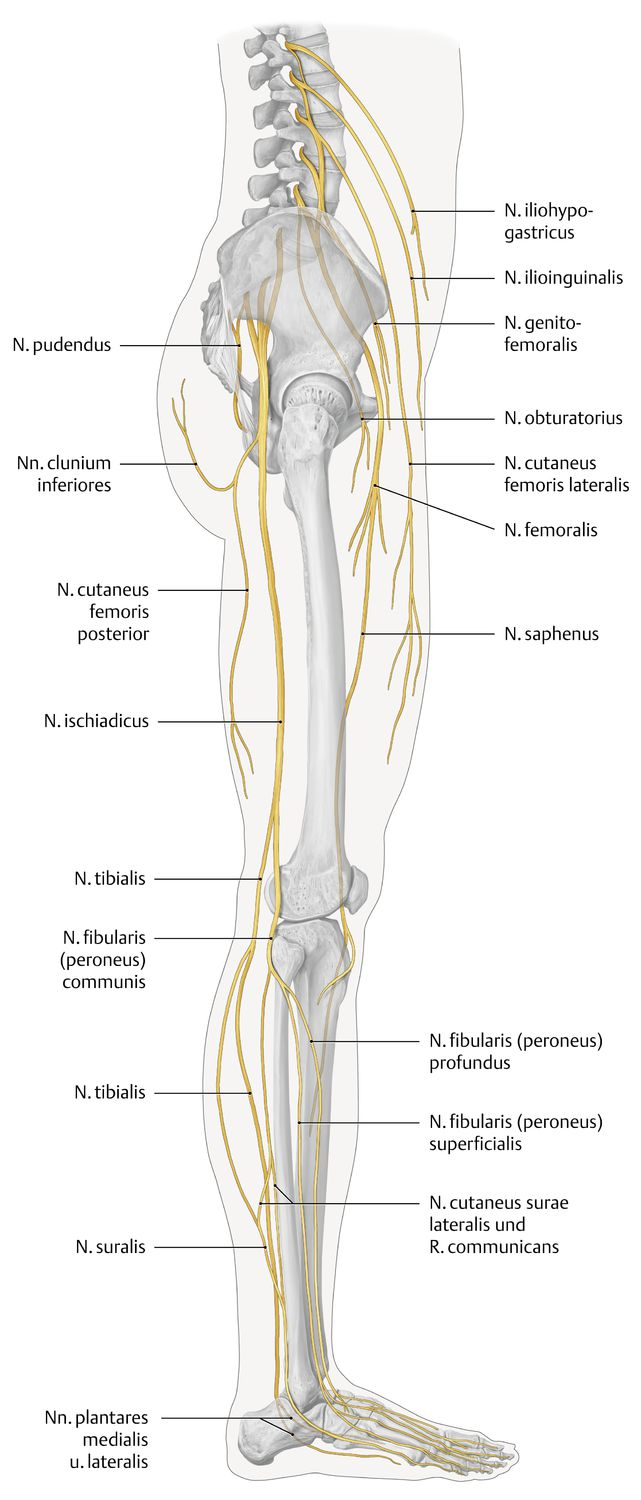
\includegraphics[width=\linewidth]{anat_sagittal}
            \label{fig:subfig:anat_sagittal}
        }
    \end{minipage}
    \begin{minipage}[c][0.9\textheight][t]{.5\textwidth}
        \centering
        \vspace*{\fill}
        \subfloat[]
        {
            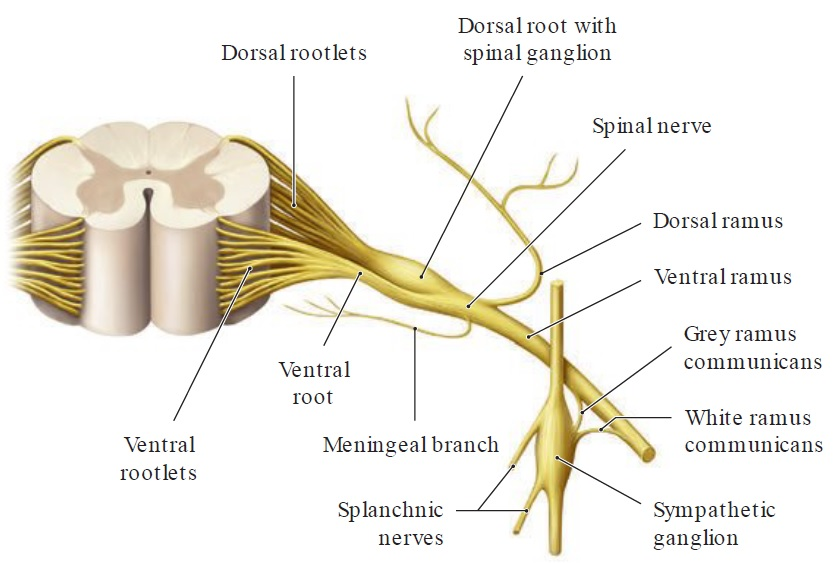
\includegraphics[width=\linewidth]{anat_spinal}
            \label{fig:subfig:anat_spinal}
        }
        \vfill
        \subfloat[]
        {
            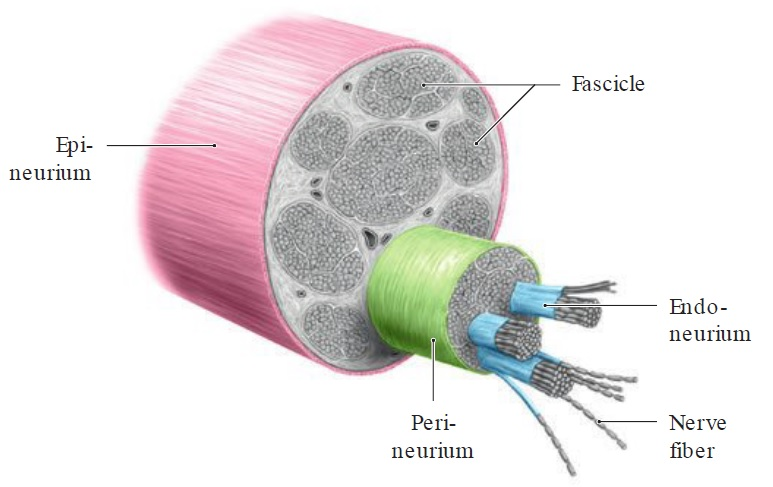
\includegraphics[width=\linewidth]{anat_nerve}
            \label{fig:subfig:anat_nerve}
        }
    \end{minipage}
    \vspace*{-0.3cm}
    \caption[Anatomy of the Peripheral Nervous System]{The anatomy of the \gls{pns} at different scales. \textbf{(a)} Nerves of the \gls{pns} of the lower limb, including the \gls{n.} ischiadicus. The \gls{n.} ischiadicus splits into the \gls{n.} tibialis and the \gls{n.} fibularis proximal of the knee.  \textbf{(b)} Sensory nerves enter the spinal cord dorsal and motor nerves exit the spinal cord ventral. \textbf{(c)} Structure of a peripheral nerve. Image \textbf{(a)} from~\cite{Schunke2014PrometheusAnatomie} and \textbf{(b)}, \textbf{(c)} from~\cite{Schunke2015THIEMEAnatomy}.}
    \label{fig:anat}
\end{figure}

\begin{figure}[htbp]
	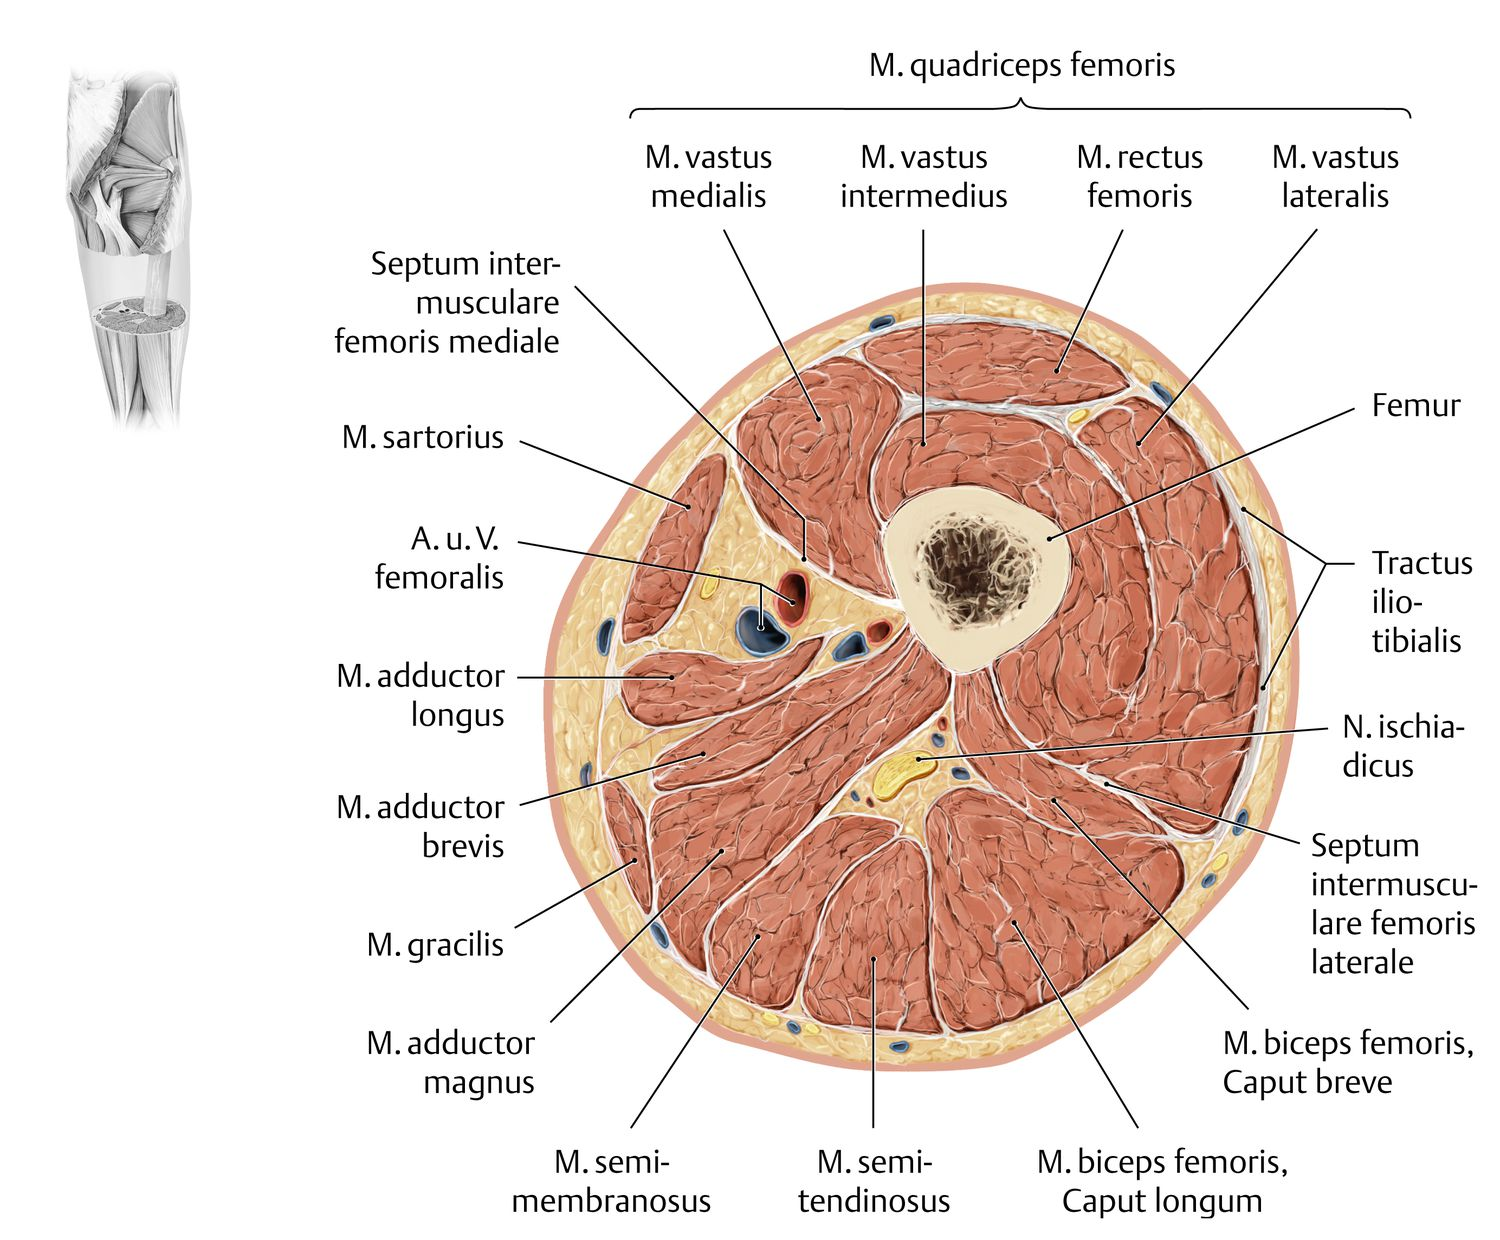
\includegraphics[width=\textwidth]{anat_axial}
    \caption[Cross-section of the Right Thigh]{Cross-sectional view of the right thigh with the femur, muscles, blood vessels, and \gls{n.} ischiadicus. Image from~\cite{Schunke2014PrometheusAnatomie}.}
    \label{fig:anat_axial}
\end{figure}

\subsection{Peripheral Neuropathies}
The prevalence of peripheral neuropathies is approximately 2.4 \% and rising to 8.0 \% with the age $\geq$ 55 years according to \cite{Martyn1997EpidemiologyNeuropathy}. A more recent study~\cite{Gregg2004PrevalenceSurvey} rises the prevalence of peripheral neuropathies with the age $\geq$ 40 years even to 14.8 \%. The most common cause of peripheral neuropathies in the developed world is diabetes mellitus. Other causes include metabolic disorders, infections, toxins, and drugs \cite{England2004PeripheralNeuropathy,Hughes466}.
Peripheral neuropathies can be caused by the damage of the axons or by demyelination, which hinders the fast transmission of neural signals. 
As the \gls{ans} controls almost every organ, a wide range of symptoms can arise when it is damaged. Damage to motor nerves may give rise to movement impairment or muscle weakness~\cite{Mohassel2015}. Damage to sensory nerves can be the cause of pain or altered sensation.

\subsection{State-of-the-Art Diagnosis}
Diagnosis and assessment of peripheral neuropathies rely on neurological examinations, which include clinical history, physical examination, and \gls{eds}. Biopsies, which are common in other medical fields, e.g., for the diagnosis or examinations of tumors and pathologies, are rarely conducted due to the irreversible damage to the nerves. \gls{eds} of the \gls{pns} are clinical tools that aid in the diagnostic assessment of patients with signs and symptoms of peripheral neuropathies~\cite{Mohassel2015}. \gls{eds} are used as an extension to the physical examination, and their primary goal is to help with the localization of peripheral nerve lesions and to assess their distribution (focal, multifocal, or generalized; one segment, multiple segments, or diffuse within the nerve)~\cite{Mohassel2015}. Additionally, \gls{eds} help determining age, severity, pathology, prognosis, and can be used for treatment planning~\cite{Mohassel2015}. Many physiologic and non-physiologic factors, e.g., age, height, tissue temperature, and pathology influence \gls{eds}. Normally, \gls{eds} are composed of two different tests, \gls{ncs} and \gls{emg}, which are related and complement each other.\\

\textbf{Nerve Conduction Studies}: \gls{ncs} measure the electrical signal propagation along a given nerve. The nerve of interest is stimulated at one site, and the electrical response signal is measured at another, which can then be analyzed. Typical signal measurements for \gls{ncs} include distal latency, amplitude, conduction velocity, and late response latency. Prolonged distal and late response latency, and reduced conduction velocity can indicate degeneration of the myelin sheath. A decreased amplitude can be the indicator of axonal degeneration~\cite{Mohassel2015}. However, a correct stimulation of proximal and deeper nerves is difficult. Therefore, those nerves are typically difficult to assess with \gls{ncs}~\cite{Mohassel2015}. \\

\textbf{Electromyography}: \gls{emg} or needle \gls{emg} complements \gls{ncs}, and can help to confirm suspected pathologic processes. \gls{emg} includes the evaluation of spontaneous activity at rest and the assessment of voluntary motor units upon activation by inserting a needle into the muscle. The needle serves as electrode and locally samples electrical activity of the muscle fibers. As \gls{emg} comes with discomfort for the patient (needle insertion), and a large number of muscles which could potentially be investigated, it is important to have a detailed anatomical knowledge and a hypothesis-driven approach~\cite{Mohassel2015}.\\
As of today, \gls{eds} are the first choice for the diagnosis of peripheral neuropathies. Apparent drawbacks are the insertion of the needle during \gls{emg} and that electrical stimulation may be painful or cause discomfort. Furthermore, \gls{eds} may not be applicable to nerves situated deep in the body, stimulate only the fastest conducting nerve fibres, and may yield inconclusive results.

\subsection{Imaging of the Peripheral Nervous System}
Imaging of the \gls{pns} as a complementary diagnostic tool to the state-of-the-art diagnosis has gained increasing attention in recent years. The following modalities are usually used to image the \gls{pns}~\cite{Ohana2014CurrentSystem}.\\

\textbf{\gls{us}}: \gls{us} can be used for examination because the nerves of the \gls{pns} usually are very superficial. Figure~\ref{fig:subfig:imag_us} shows \gls{us} images of the \gls{n.} ulnaris. \gls{us} is cheap and widely available. Advantages of \gls{us} are the large \gls{fov}, and that there are no contraindications. \gls{us} however, is very operator dependent and also suffers from poor contrast resolution of for the nerves. Furthermore, there are limitations to the applicability of \gls{us} in deep or difficult accessible anatomical areas~\cite{Ohana2014CurrentSystem}.\\

\textbf{\gls{mrn}}: \gls{mrn} is \gls{mri} tailored to the imaging of peripheral nerves. Optimized MR sequences allow for better contrast between the nerves and their surrounding tissues. Phased-array coils and high field imaging (e.g., 3~Tesla or higher) increase signal-to-noise ratio as well as the spatial resolution, allowing nerves to be examined. \gls{mrn} has excellent soft-tissue contrast and a higher \gls{fov} than \gls{us}. The resulting images are \gls{3d} and even deeply situated nerves can be imaged. Typically, the \gls{mrn} protocols make use of T1-weighted spin-echo sequences (excellent spatial resolution), T2-weighted spin-echo sequences (good contrast resolution), and "neurography" sequences, which are strongly T2-weighted using long echo times and fat signal suppression~\cite{Ohana2014CurrentSystem}. \gls{mrn}, however, is rather costly, has limited availability and acquisition may take a long time. Figure~\ref{fig:subfig:imag_mrn} depicts \gls{mrn} images of the \gls{n.} ulnaris at the wrist.\\

\textbf{\gls{ct}}: \gls{ct} is not as often used as the previous imaging modalities for peripheral nerves but it has some distinct benefits. \gls{ct} is useful in diagnosing spinal nerve compressions, and is often combined with \gls{ct} Myelography. \gls{ct} has a good spatial resolution, and excellent bone contrast. However, although large nerve trunks are often visible, the low contrast resolution does not enable a detailed examination of the neuronal microstructure~\cite{Ohana2014CurrentSystem}. Another disadvantage is the inherent irradiation of the tissue. Figure~\ref{fig:subfig:imag_ct} shows a curvilinear nerve reconstruction based on a \gls{ct} angiogram.\\


\begin{figure}[htbp]
	\centering
	\subfloat[]
	{
		\label{fig:subfig:imag_us}
		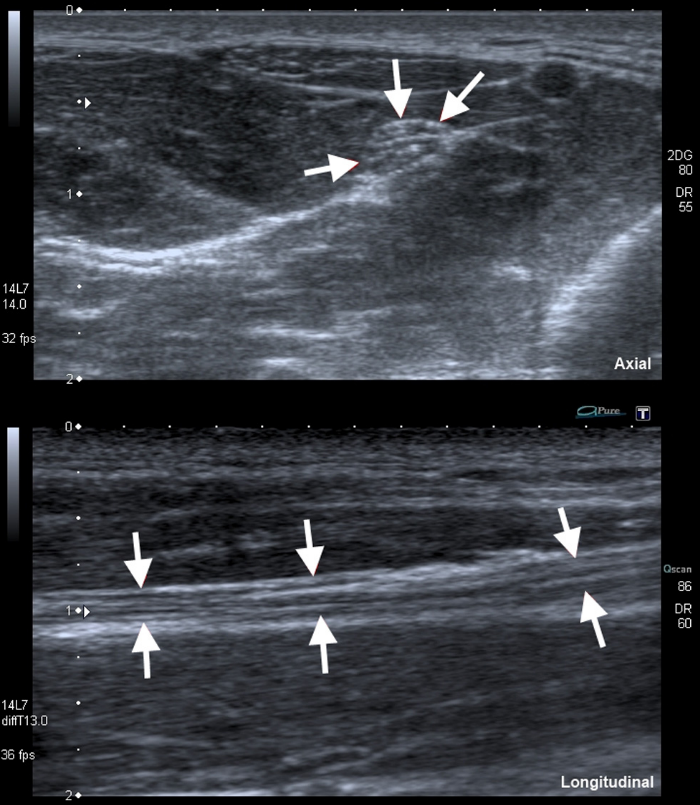
\includegraphics[width=0.48\textwidth]{imag_us}
	}
	\hfill
	\subfloat[]
	{
		\label{fig:subfig:imag_mrn}
		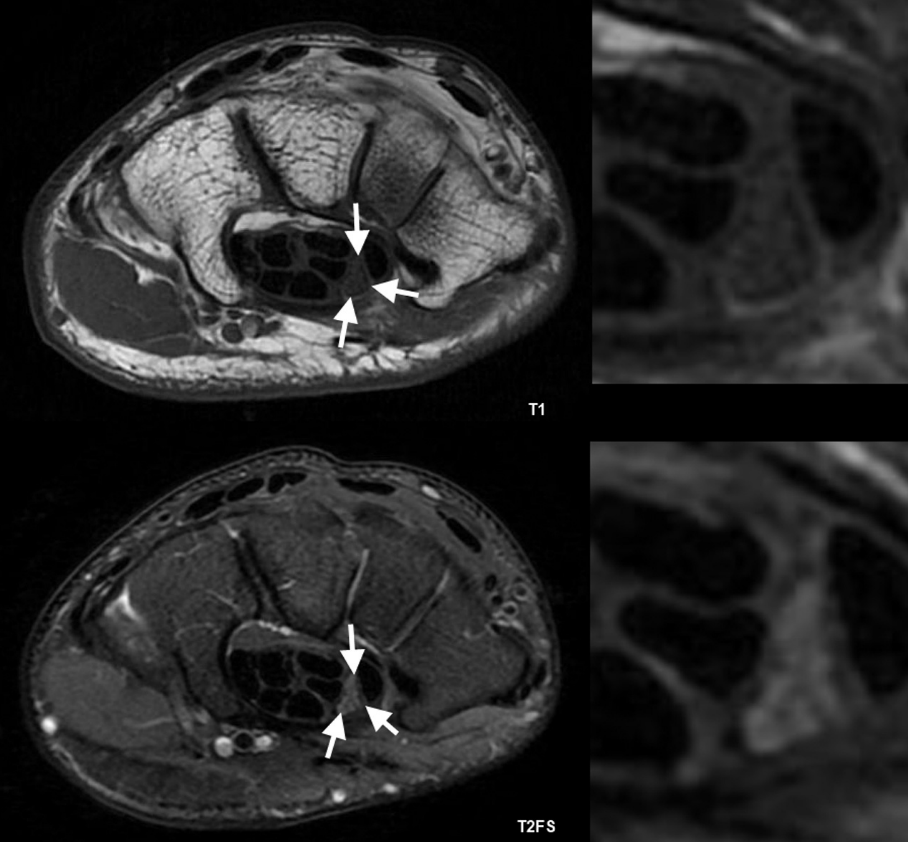
\includegraphics[width=0.48\textwidth]{imag_mrn}
	}
	\hfill
	\subfloat[]
	{
		\label{fig:subfig:imag_ct}
		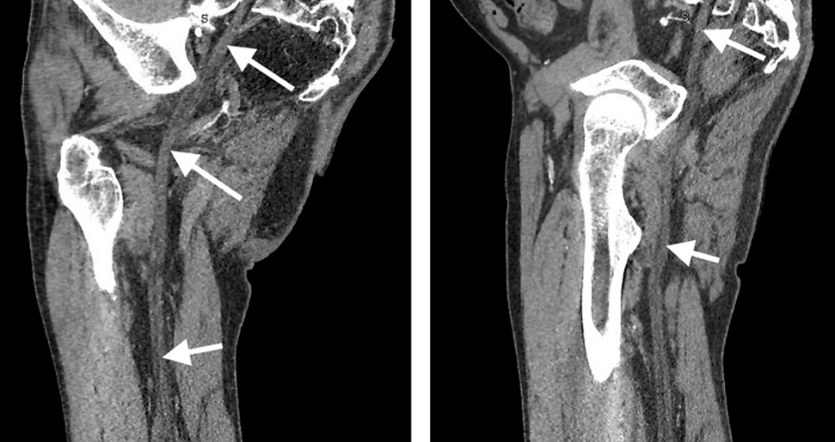
\includegraphics[width=0.7\textwidth]{imag_ct}
	}
	\caption[Modalities for Imaging of the Peripheral Nervous System]{Different modalities for \acrlong{pns} imaging. \textbf{(a)} \gls{n.} ulnaris at the wrist visible in axial (top) and longitudinal ultrasound sections. \textbf{(b)} Sagittal sections of the \gls{n.} medianus: T1-weighted image (top) and T2-weighted image with fat suppression (bottom). \textbf{(c)} Curvilinear reconstructions of the right \gls{n.} ischiaducus from a lower limb CT angiogram. Images from~\cite{Mohassel2015}.}
	\label{fig:imag_modalities}  
\end{figure}

\section{Medical Image Segmentation} \label{sec:intro_mia} % ===================================================================
Segmentation in digital image processing refers to the extraction of a target structure of interest from an image, or to partition the image into multiple segments. Segmentation results in a representation, which is easier to analyze. Typically, object boundaries or regions belonging to one semantic object are of interest. The task of segmentation, in essence, boils down to the pixel-wise assignment of object membership or more commonly class labels. Pixels belonging to the same object, i.e. share some characteristics, have the same class labels assigned.\\
Medical image segmentation usually involves the segmentation of an anatomical object of interest in some medical image, e.g., \gls{ct} or \gls{mri} image. The segmentation has to be performed manually by an expert due the required anatomical and image knowledge. Such manual segmentation is not always reproducible, means tedious work and is time-consuming. Even more so, by the fact that the medical images are often \gls{3d} images. Therefore, medical image segmentation is subject to research aiming at having automatic or semi-automatic, computer-assisted segmentation tools. However, such tools are not always able to deliver the required performance due to . Recently, deep learning-based segmentation of medical images, with the use of convolutional neural networks has become increasingly popular~\cite{Ronneberger2015U-Net:Segmentation,Tetteh2018DeepVesselNet:Volumes,Cicek20163DAnnotation,Baumgartner2017AnSegmentation,Meng2017TrackingNetwork,Milletari2016V-Net:Segmentation,BalsigerContext-awareNeurography,Kayalibay2017CNN-basedData}, and achieved or even surpassed human-level performances.

\section{Machine Learning} \label{sec:intro_mlearn} % =============================================================================
In this part, we briefly describe some fundamentals of machine learning. Machine learning is a huge topic and this section is by no means meant to be a complete overview. We rather introduce concepts and mention topics, which are related and important for our work.

\subsection{Supervised Learning} \label{sec:ml_supervised}
The principle of supervised learning is illustrated on the prediction of house prizes as a function of their living area in Figure~\ref{fig:dl_supervised}~\cite{Ng2012StanfordNotes}. In supervised learning, we train an algorithm (also called model) by providing the algorithm input-output pairs (e.g., living area of houses with their corresponding prizes). This is referred to as the training phase, and the input-output pairs are called the training set. The outputs are typically referred to as labels or targets. More formally, we define the training set as
\begin{equation}
   S_{Train} = \{(x^{(i)}, y^{(i)}); \quad i = 1,...,m\},
   \label{eq:training_set}
\end{equation}
where $(x^{(i)}, y^{(i)})$ denotes the $i$-th input-output pair consisting of the data $x$ and the label $y$. Let $\chi$ and $\upsilon$ denote the space of input and output values, respectively. In this example, $\chi = \upsilon = \mathbb{R}$. The aim of the training phase is to let the algorithm learn a meaningful relationship between the inputs and outputs of our training set. Therefore, we aim learn a mapping $h : \chi \mapsto \upsilon$, parameterized by a set of models weights~$\textbf{W}$, which is \textit{good} for all pairs in $S_{Train}$, hence
\begin{equation}
   y^{(i)} = h(x^{(i)}; \mathbf{W}); \quad i = 1,...,m,
   \label{eq:model}
\end{equation}
is approximatively valid for all training pairs. We call $h(x^{(i)}; \mathbf{W})$ our model, parameterized by the model's weights~$\textbf{W}$. Depending on the type of mapping, $\mathbf{W}$ is typically a matrix and we therefore, write it in bold capital letter. If the training is able to find a meaningful relation, the model can be used to make predictions on previously unseen input data $\hat{x}$.\\
If the output, we are trying to predict, is continuous, such as in the housing example, the problem is called a \textbf{regression problem}. We could also have the situation where we wanted to predict whether the dwelling is an apartment or a house, given the living area. The predicted output would, therefore, be discrete and we would call this a \textbf{classification problem}.\\
Supervised learning gets its name for the reason that the algorithm always learns on input-output pairs. Typically, the outputs  are the result of (laborsome) labeling work done by a person. This is the largest drawback of supervised learning. There exist ways to use unlabeled data in conjunction with labeled data, referred to as semi-supervised learning. Learning on input data without labels corresponds to finding patterns and structures in the input space and is referred to as unsupervised learning. Typical examples for unsupervised learning algorithms are \gls{pca} and $k$-means clustering~\cite{Goodfellow2016DeepLearning}.\\
For the housing example, one could expect a linear relationship, between the living area of a house and its prize. If this was indeed true, we could make robust predictions with a simple linear model, i.e. $y^{(i)} = h(x^{(i)}; W) = Wx^{(i)} + b$, only incorporating the living area. Note that in this case, the parameters of our model are a single scalar weight $W$ and a bias term $b$.
However, one could argue that the number of rooms or the location, each with its unknown weight, also influence the dwelling's prize. These influences are typically called features. There was and still is a whole science around finding good features to solve learning problems, which often relied on hand-crafting these features. The main drawback of any learning algorithm relying on hand-crafted features is that the algorithm is inherently constrained by the imagination and ability of the engineer to find and implement good features.

\begin{figure}[htbp]
    \centering
	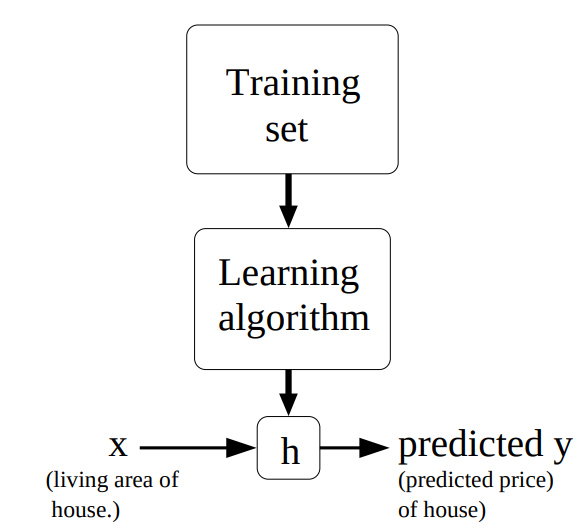
\includegraphics[width=0.5\textwidth]{supervised_learning}
    \caption[Supervised Learning]{The principle of supervised learning illustrated on the example of predicting house prices y depending on the living area x. Suppose we have $m$ area-price pairs, which we name our training set: $\{(x^{(i)}, y^{(i)}); \quad i = 1,...,m\}$. We let $\chi$ and $\upsilon$ denote the space of input and output values, respectively. In this example, $\chi = \upsilon = \mathbb{R}$. In supervised learning we aim to learn a function (also called mapping) $h : \chi \mapsto \upsilon$, which makes reasonable prize prediction y for a given new house area $\hat{x}$. We use the training set to learn $h$. Image and example taken from~\cite{Ng2012StanfordNotes}.}
    \label{fig:dl_supervised}
\end{figure}

\subsection{Training}
In the previous section, we defined that the model $h(x^{(i)}; \mathbf{W})$ is parametrized by the set of weights $\textbf{W}$. During the training phase of the model, we adjust $\textbf{W}$ in order for the model to make better predictions on the training set. Formally, we want to solve the optimization problem
\begin{equation}
   \mathbf{W}^{*} = \argmin_\textbf{W} \sum_{i=1}^{m} L(h(x^{(i)}; \mathbf{W}), y^{(i)}),
   \label{eq:optimization}
\end{equation}
where $L(\cdot)$ denotes a loss function. The loss function is a metric we have to choose, which calculates the error between the correct label $y^{(i)}$ and the prediction $\hat{y}^{(i)}$ our model made. The loss function is often also referred to as cost function. $\mathbf{W}^{*}$ denotes the solution for the mentioned optimization problem and, consequently, is the set of weights which results in the smallest error in our training set. Training of a model corresponds to iteratively decreasing the training error.\\
A loss function typically used for classification problems with $k$ classes, a prediction vector $\mathbf{h}^{(i)} \in \mathbb{R}^k$ and a categorial label vector $\mathbf{y}^{(i)} \in \{0,1\}^{k}$, is the \textbf{cross-entropy} loss

\begin{equation}
    L(\mathbf{h}^{(i)}, \mathbf{y}^{(i)}) = -\sum_{c=1}^{k}\mathbf{y}_{c}^{(i)} \log(f(\mathbf{h}^{(i)})_c),
    % L(\mathbf{h}^{(i)}, \mathbf{y}^{(i)}) = -\mathbf{y}^{(i)} \log(f(\mathbf{h}^{(i)})),
    \label{eq:cross_entropy_multi}
\end{equation}
with $f(\cdot)$ being the \textbf{softmax} function
\begin{equation}
   f(\mathbf{h}^{(i)}) = \frac{\exp\mathbf{h}^{(i)}}{\sum_{j} \exp{\mathbf{h}^{(i)}_{j}}},
   \label{eq:softmax}
\end{equation}
which squashes the predictions into a vector of values between zero and one that sum to one. The corresponding cross-entropy loss for a binary classification problem is
\begin{equation}
    L({h}^{(i)}, {y}^{(i)}) = -{y}^{(i)} \log(\sigma({h}^{(i)})) - (1- {y}^{(i)})\log(1- \sigma({h}^{(i)}))
    %L({h}^{(i)}, {y}^{(i)}) = -{y}^{(i)} \log(\sigma({h}^{(i)}))
    \label{eq:cross_entropy_binary}
\end{equation}
with $\sigma(\cdot)$ being the \textbf{sigmoid} function
\begin{equation}
   \sigma({h}^{(i)}) = \frac{1}{1 + \exp{(-{h}^{(i)})}}.
   \label{eq:sigmoid}
\end{equation}

In order to solve Equation~\ref{eq:optimization}, optimizers are used. Optimizers, such as \gls{sgd}~\cite{Goodfellow2016DeepLearning} and Adam~\cite{Kingma2014Adam:Optimization} use the gradient to find $\textbf{W}^*$. The gradient depends on the model and the chosen loss function, and corresponds the first-order derivatives of the individual inputs with respect to the outputs.\\

A common problem in machine learning is under- and overfitting (Figure~\ref{fig:under_over_fitting}). To solve a learning problem, we have to choose a model first. The model's representational power, hence the ability to fit a wide variety of functions, is called capacity~\cite{Goodfellow2016DeepLearning}. If the model's capacity is too low for the task at hand, it cannot model the relationship between the input and output. This is called underfitting. On the contrary, if the models capacity is too high, it can start to memorize the data it was trained upon (including the data's statistics) rather than learning structures or relationships. This results in a bad performance on new, unseen data, hence bad generalization, which is called overfitting.

\begin{figure}[htbp]
    \centering
	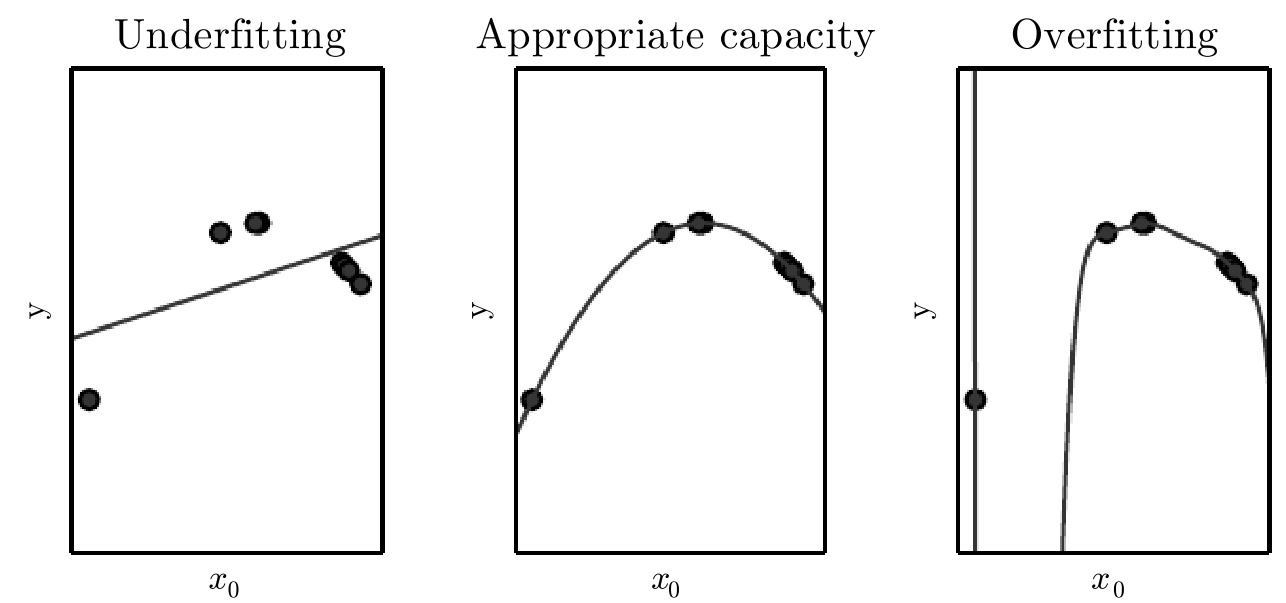
\includegraphics[width=0.8\textwidth]{under_over}
    \caption[Under- and Overfitting]{The problem of under- and overfitting of machine learning algorithms. The points were generated by random sampling a quadratic function. In the left image, a model with low capacity (a line) is not able to correctly capture the structure of the points. The center image shows that a quadratic model would generalize well to unseen points. The right image shows that a 9\textsuperscript{th} degree polynomial would generalize bad to new points despite passing through all points. Image and example taken from~\cite{Goodfellow2016DeepLearning}.}
    \label{fig:under_over_fitting}
\end{figure}

\subsection{Deep Learning \& Convolutional Neural Networks}
With the growing amount of labeled data, gathered in large datasets, and increasing computational performance using \gls{gpu}s, the creation and training of models, called neural networks, with much larger capacity became possible. The most significant advantage of those models was that (given enough training data) it was now possible to train them directly on raw, unprocessed data, rather than on human-engineered features.\\
\gls{cnn}, a class of neural network mostly used to analyze visual imagery, achieved new levels of performances in computer vision tasks and challenges \cite{Krizhevsky2012ImageNetNetworks,Simonyan2014VeryRecognition,Szegedy2014GoingConvolutions,He2015DeepRecognition,Zeiler2014VisualizingNetworks}. 
CNNs and neural networks in general, use a cascade of multiple layers of units which can process and transform data. Each layer takes the previous layer's output as an input. \gls{cnn}s, in contrast to regular neural networks, assume that the input data has some spatial relationship, hence the popular use of \gls{cnn}s for computer vision tasks. Because a \gls{cnn} consists of several sequential convolutional layers, the learned filters deeper in the network can act as detectors for higher semantical features. Therefore it can learn multiple levels of representations, which correspond to multiple levels of abstraction. During training, a \gls{cnn} learns the convolutional filters, which act as detectors for features present in the data. It basically builds its internal filter bank to extract information. Figure~\ref{fig:mlearn_weights} shows the learned filters in the first layer of an AlexNet trained for natural image classification~\cite{Russakovsky2015ImageNetChallenge}. Note that the learned weights resemble filters for edge or blob detection (sobel operator~\cite{Sobel1990AnOperator}, Laplacian of Gaussian~\cite{Marr187}) widely used in computer vision.\\
A typical \gls{cnn} is built as a sequence of multiples of the following layers~\cite{KarpathyStanfordRecognition}. Each layer transforms the activations of the previous layer into new activations, through a differentiable function.\\
We briefly summarize the most used type of layers.

\textbf{Convolutional Layer:} Layer which contains the learnable weights. The learnable weights form filters, which are used for information extraction. Parameters for a convolutional layer are typically the kernel size of the filters and the number of individual filters (also referred to as channels or features).\\

\textbf{ReLU Layer:} Applies the Equation~\ref{eq:relu} to each of the outputs of the previous layer. This results in thresholding at zero. Other typical activation functions are the sigmoid (Equation~\ref{eq:sigmoid}) or the tanh function.\\
\begin{equation}
   ReLU({h}^{(i)}) = \max(0, {h}^{(i)}).
   \label{eq:relu}
\end{equation}

\textbf{Pooling Layer:} A pooling layer performs a down-sampling operation along the spatial dimensions. Typically max-pooling is used, which only lets the maximum activation through. Pooling helps prevent overfitting by reducing the number of parameters in a network.\\

\textbf{Transposed Convolutional Layer:} A transposed convolutional layer performs and up-sampling operation along the spatial dimensions and is typically used as the inverse operation of the pooling layer.\\

\textbf{Dropout layer:} Randomly deactivates some of the activations of the previous layer. Dropout~\cite{Srivastava2014Dropout:Overfitting} is a type of regularization and thus aims to reduce the overfitting problem.\\

\textbf{Normalization Layer:} Different types of normalization layers have been proposed, including Batch Normalization~\cite{SergeyIoffe2015BatchNormalization}. They all normalize the activations in some way.
 
\begin{figure}[htbp]
	\centering
	\subfloat[]
	{
		\label{fig:subfig:mlearn_nn}
		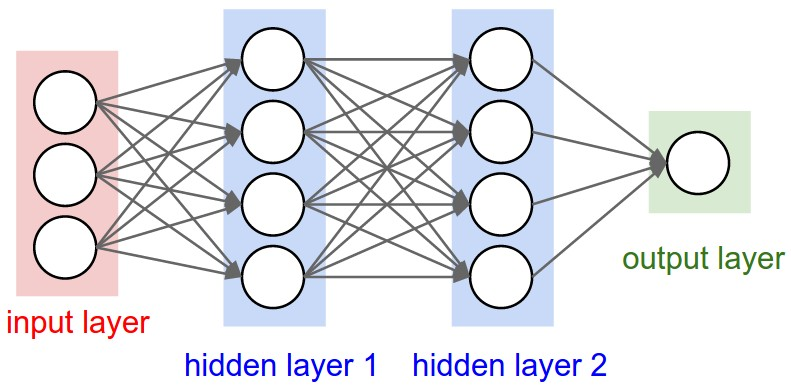
\includegraphics[width=0.48\textwidth]{mlearn_neural_network}
	}
	\hfill
	\subfloat[]
	{
		\label{fig:subfig:mlearn_cnn}
		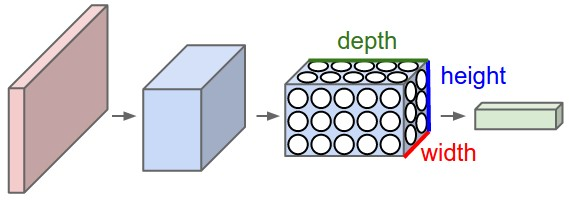
\includegraphics[width=0.48\textwidth]{mlearn_cnn}
	}
	\caption[Regular Neural Networks and Convolutional Neural Networks]{\textbf{(a)} Fully-connected neural network where each neuron of a layer is connected to every neuron of the previous layer. \textbf{(b)} CNN where the weights are organized in a \gls{3d} way. Each of the nodes is only locally connected to nodes of the previous layer. The main motivation behind this is that a learned filter (e.g. edge detector) is useful over the whole image. Images from~\cite{KarpathyStanfordRecognition}.}
	\label{fig:mlearn_nn_cnn}  
\end{figure}


\begin{figure}[htbp]
    \centering
	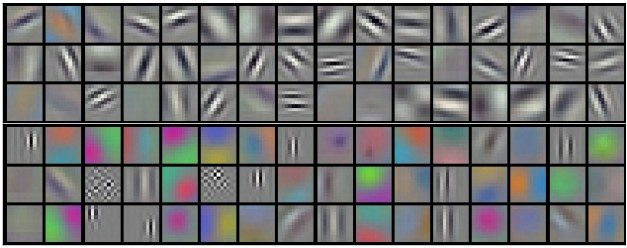
\includegraphics[width=0.8\textwidth]{mlearn_weights}
    \caption[Learned Weights of a trained AlexNet]{Learned convolutional filters of the first layer of an AlexNet trained for natural image classification~\cite{Krizhevsky2012ImageNetNetworks}. The learned filters act as detectors for high-frequency gray-scale features, mostly edges, and low-frequency color features.}
    \label{fig:mlearn_weights}
\end{figure}

\section{Related Work} % =================================================================================
As of today, there is relatively low interest from the scientific community in the segmentation of the nerves of the \gls{pns}. Felisaz et al.\cite{Felisaz2016NerveMicro-neurography} proposed a semi-automatic method to segment and measure the volumes of different compartments of the tibial nerve based on \gls{mrn} images. They measured fascicular volume, epineural volume, nerve volume, and the \gls{fnr}. They also calculated the inter- and intra-observer agreements. They concluded that the method is reproducible and \gls{fnr} is a novel biomarker, which may help in the diagnosis of peripheral neuropathies.
In \cite{Felisaz2017MRNeuropathy.} they further studied the assessment of morphometric ultrastructural changes in nerves affected by diabetic peripheral neuropathy. As in their previous work, they used a semi-automated technique of tissue segmentation to calculate nerve volumes, fascicle volumes, the \gls{fnr}, and the \gls{csa}. They noted increased nerve volumes and decreased \gls{fnr} in patients with diabetic peripheral neuropathy. The fascicle volume was increased in patients with moderate to severe diabetic peripheral neuropathy.
In their recently published work \cite{FelisazTextureNeuropathy} they applied texture analysis to MRN images and concluded that texture analysis might help to discriminate between normal and pathologic nerves.\\
Balsiger et al. investigated the use of hand-crafted features for the semi-automatic segmentation of the peripheral nerves with \gls{rf}. The \gls{rf}, was trained in a supervised fashion on hand-crafted features on a dataset consisting of \gls{mrn} images. Besides intensity-based features, the approach also incorporated a context feature. For this context feature, the user annotated the centers of the proximal and distal ends of the sciatic nerve by a single voxel in the MRN image. In case the branching of the sciatic nerve is included in the MRN image, the user annotated additionally its location. The nerve centers for the non-annotated slices were interpolated via first-order B-spline. The final context feature was obtained by the Euclidean distance from each pixel to the center of the nerve in each slice. Although the user annotation was limited, the clinical adoption of this approach is still questionable due to the user interaction. Motivated by the issue, their recent work~\cite{Balsiger2018SegmentationApproach} included a  fully-automatic deep learning-based method to segment the peripheral nerves. A \gls{fcnn} based on the fully-convolutional DenseNet~\cite{Huang2017DenselyNetworks} was trained on MRN images and evaluated. They achieved partial human-level performance compared to an inter-rater variability study. However, their approach based on a \gls{2d} \gls{fcnn} approach, which might be questionable due to the most recent advancements in medical image segmentation regarding \gls{3d} segmentation approaches. 

\section{Hypothesis} % ===================================================================================
Quantitative biomarkers for peripheral neuropathies, such as \gls{csa} and the \gls{fnr}, require an accurate segmentation of the peripheral nerve. Because manual segmentation is clinically unfeasible, computer-assisted segmentation is preferred.
For this reason, we aim to segment the sciatic nerve of the \gls{pns} fully-automatically from \acrshort{mrn} images, using a deep learning-based approach. Therefore, our first hypothesis is\\

\textit{Deep learning-based segmentation of peripheral nerves from \gls{mrn} images is possible with human-level performance.} \\

MRN images are \gls{3d} and the sciatic nerve is a \gls{3d} structure. Hence, our second hypothesis is\\

\textit{\gls{3d}-contextual information increases the segmentation accuracy.}

\section{Aim \& Structure of the Thesis} % ===============================================================
The aim of the thesis was to develop a deep learning-based approach to segment the sciatic nerve from \gls{mrn} images and to investigate the impact of \gls{3d} context on the segmentation performance.\\
\begin{itemize}
    \item Chapter~\ref{chap:methods} presents the used materials and the developed methods. It elaborates on how we designed and trained our neural networks, dealt with the problem of overfitting, and how we applied post-processing. Furthermore, the conducted experiments are defined.
    \item Chapter~\ref{chap:results} presents the obtained results for the proposed experiments. Further detailed results can be found in Appendix~\ref{app:results}.
    \item Chapter~\ref{chap:discussion_and_conclusions} discusses the results and conclusions are drawn.
    \item Chapter~\ref{chap:outlook} presents a visionary outlook.
\end{itemize}

\endinput
\chapter{Materials \& Methods} \label{chap:methods}
This chapter describes the materials and the methods we used for the segmentation of the peripheral nerves. More specifically, Section ~\ref{sec:materials} provides an detailed insight into the patient and volunteer \gls{mrn} images as well as the software \& frameworks we use. Sections ~\ref{sec:preprocessing} to ~\ref{sec:postprocessing} describe the main part of the segmentation pipeline. Section ~\ref{sec:evaluation} concludes this chapter by showing how we evaluated the segmentation pipeline.

\section{Materials} \label{sec:materials}

\subsection{Patient \& Healthy Volunteer Data}
Patients with clinically and electrophysiologically diagnosed neuropathy and healthy volunteers receiving a \gls{mrn} examination between 2013 and 2017 at the Inselspital, Bern University Hospital, were enrolled in a registry. After the approval by the local ethical committee, and informed consent was obtained from all participants, we retrospectively selected 52 \gls{mrn} cases, separated into a patient cohort with diagnosed neuropathy (n = 42, 21 female, 21 male; 55.7 $\pm$ 15.7 years) and a healthy volunteer cohort (n = 10, 4 female, 6 male; 25.0 $\pm$ 2.6 years).\\
All images were taken from the anatomical region of the thigh and contain parts of the sciatic nerve. While the images for the volunteers were all taken at the distal thigh, the images for the patients originate from variable locations between the distal thigh up to the head of the femur. The images taken more distally typically include the branching of the sciatic nerve into the fibular and tibial nerve. Some images, taken more proximally, do not include the branching.\\
Although not used in this work, further MRN images from different anatomical regions (upper \& lower arm, lower leg) are available for the volunteer cohort. The upper leg \gls{mrn} images of the six healthy volunteers which Balsiger et al.~\cite{Balsiger2016DevelopmentApproaches} used for their work, are also part of the dataset.\\

\subsubsection{MRN Sequences} \label{dataset_mrn}
Each MRN case consists of a low-resolution T2-weighted sequence with fat suppression using \gls{ir} (Figure~\ref{fig:subfig:IR}) and a high-resolution T2-weighted sequence without fat suppression (Figure~\ref{fig:subfig:T2}). We refer in this work to the corresponding \gls{mrn} images with IR and T2, respectively. The images were acquired with a 15-channel knee coil using a 3 Tesla Siemens MAGNETOM Verio (Siemens Healthcare GmbH, Erlangen, Germany). Table~\ref{tab:dataset} summarizes the \gls{mrn} sequence and acquisition properties.

\begin{table}[htbp]
   \centering
   \caption[MRN Image Acquisition Properties]{Image and acquisition properties for the IR and T2 sequences.}
   \begin{tabular}{l*{3}{r}}
      \toprule
      Property & Unit & IR & T2 \\
      \midrule
      Resolution\footnotemark\footnotemark & voxels & $60 \times 220 \times 256$ & $60 \times 330 \times 384$ \\
      Voxel size\footref{fn:dims} & \si{\milli\metre\cubed} & $4.00 \times 0.78 \times 0.78$ & $4.00 \times 0.52 \times 0.52$ \\
      Slice distance & \si{\milli\metre} & 4.40 & 4.40 \\
      Repetition time & \si{\milli\second} & 4500 & 4690 \\
      Echo time & \si{\milli\second} & 32 & 82 \\
      Inversion time & \si{\milli\second} & 220 & - \\
      Flip angle & \si{\degree}  & 120 & 134 \\
      \bottomrule
   \end{tabular}
   \label{tab:dataset}
\end{table}

\addtocounter{footnote}{-2}
\stepcounter{footnote}\footnotetext{\label{fn:dims}Dimensions $z \times y \times x$ in axial, sagittal and coronal direction.}
\stepcounter{footnote}\footnotetext{The patient and volunteer subjects typically consist of 60 and 30 axial slices, respectively. There are some subjects which have fewer axial slices.}

\begin{figure}[htbp]
	\centering
	\subfloat[]
	{
		\label{fig:subfig:IR}
		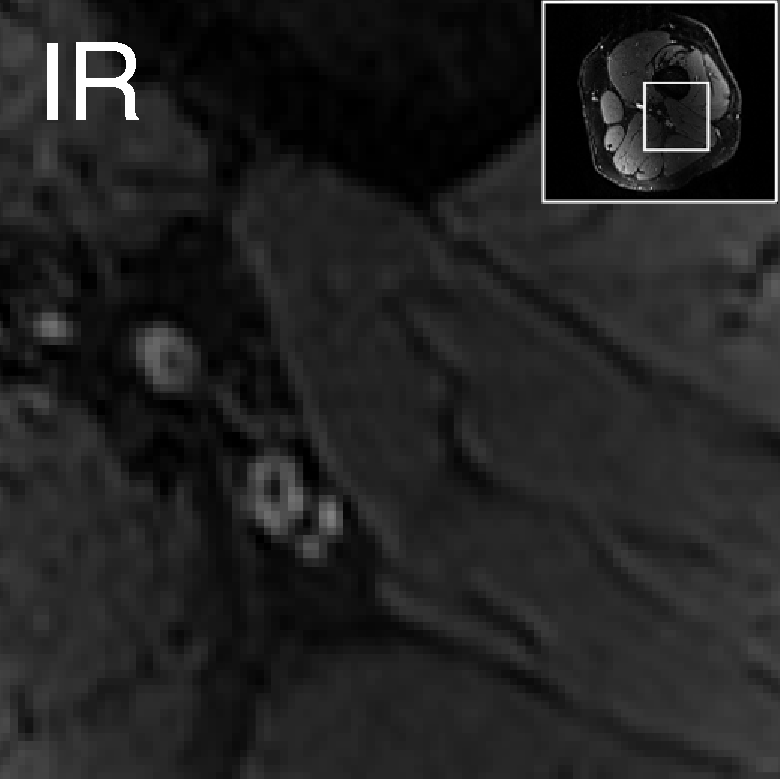
\includegraphics[width=4cm]{channel_IR}
	}
	\hfill
	\subfloat[]
	{
		\label{fig:subfig:T2}
		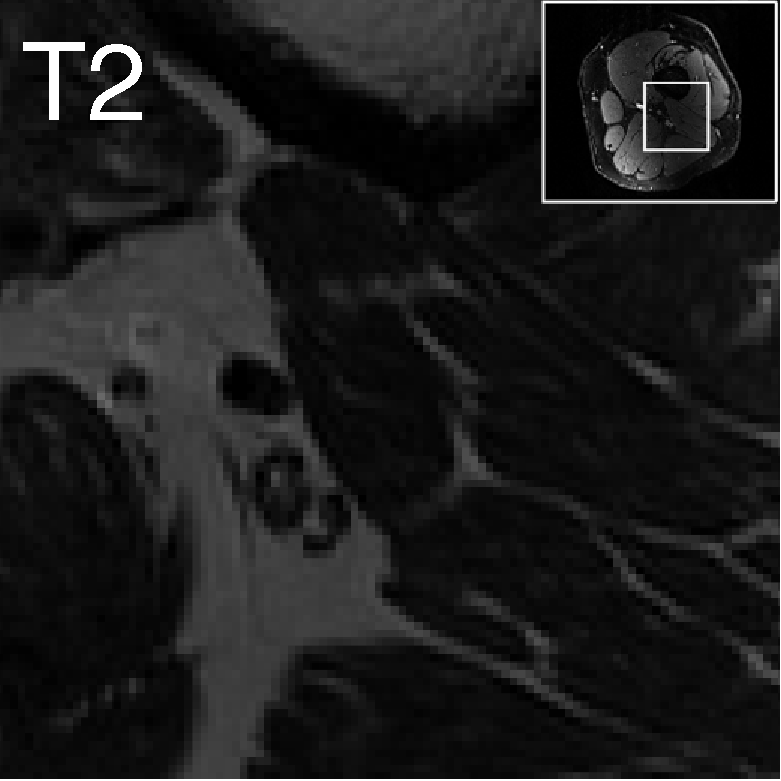
\includegraphics[width=4cm]{channel_T2}
	}
    \hfill
	\subfloat[]
	{
		\label{fig:subfig:GT}
		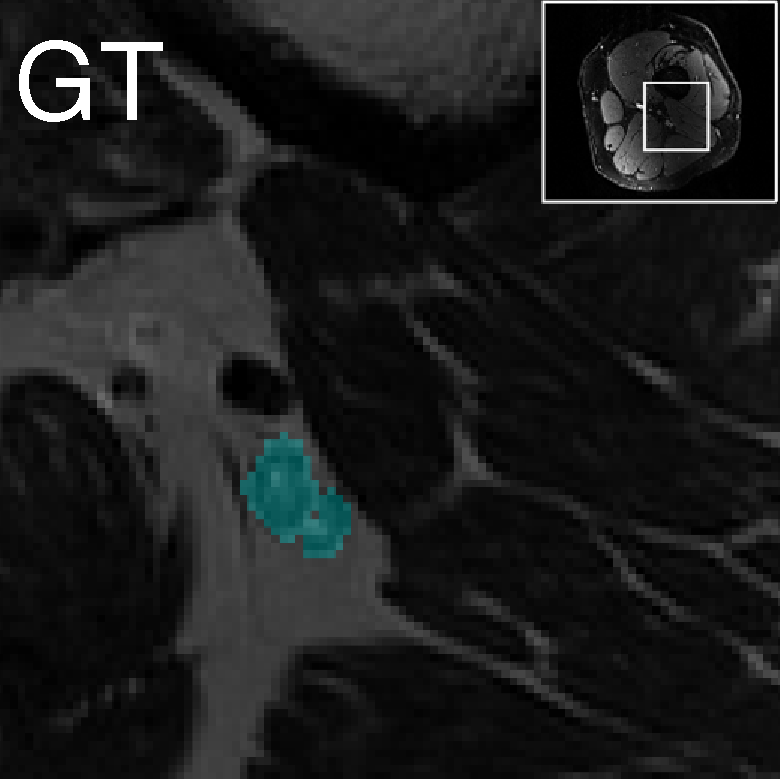
\includegraphics[width=4cm]{channel_GT}
	}
	\caption[Sections of MRN Sequences]{Axial image sections of the sciatic nerve proximal to the knee: \textbf{a)} Low-resolution T2-weighted image with fat suppression using \gls{ir}. \textbf{b)} High-resolution T2-weighted image without fat suppression. \textbf{c)} High-resolution T2-weighted image with annotated sciatic nerve. Note that the nerve has a similar appearance as blood vessels in the T2 image.}
	\label{fig:sequences}  
\end{figure}

\subsubsection{Manual Ground Truth Segmentation} \label{dataset_gt}
For each MRN case, three physicians, experienced in clinical, electrophysiological, and imaging-based assessment of neuromuscular diseases (Olivier Scheidegger (OS), senior neurologist and neuroradiologist > 14 years; Benedikt Wagner (BW), neuroradiologist > 4 years; Lorenz Grunder (LG), neuroradiologist > 2 years) manually segmented the sciatic nerve, including its distal branches the tibial and fibular nerve. The nerve segmentations were performed by each physician individually on the T2-weighted images, allowing the study of the inter-rater agreement. The segmentations were performed with the ITK-SNAP~\cite{py06nimg} software using the polygon or paintbrush tool. The descriptive statistics of the ground truth segmentations are summarized in Table~\ref{tab:ground_truths}. Important to point out is that the number of voxels belonging to the sciatic nerve only account for $0.14 \pm 0.05$ \% of the total image voxels. Figure~\ref{fig:gt_render} shows a 3D-rendering of a sciatic nerve, including the branching, based on the ground truth segmentation of OS.\\
We obtained a consensus ground truth segmentation, from now on referred to as GT, by the combination of the three expert ground truths via majority voting (GT in Table~\ref{tab:ground_truths}): A voxel was labelled sciatic nerve class if at least two rater segmented it. In our case the obtained consensus ground truth is identical to the result that one would have received by applying the \gls{staple} algorithm~\cite{Warfield2004SimultaneousSTAPLE}, which is a common algorithm for label fusing.\\

\begin{figure}[htbp]
	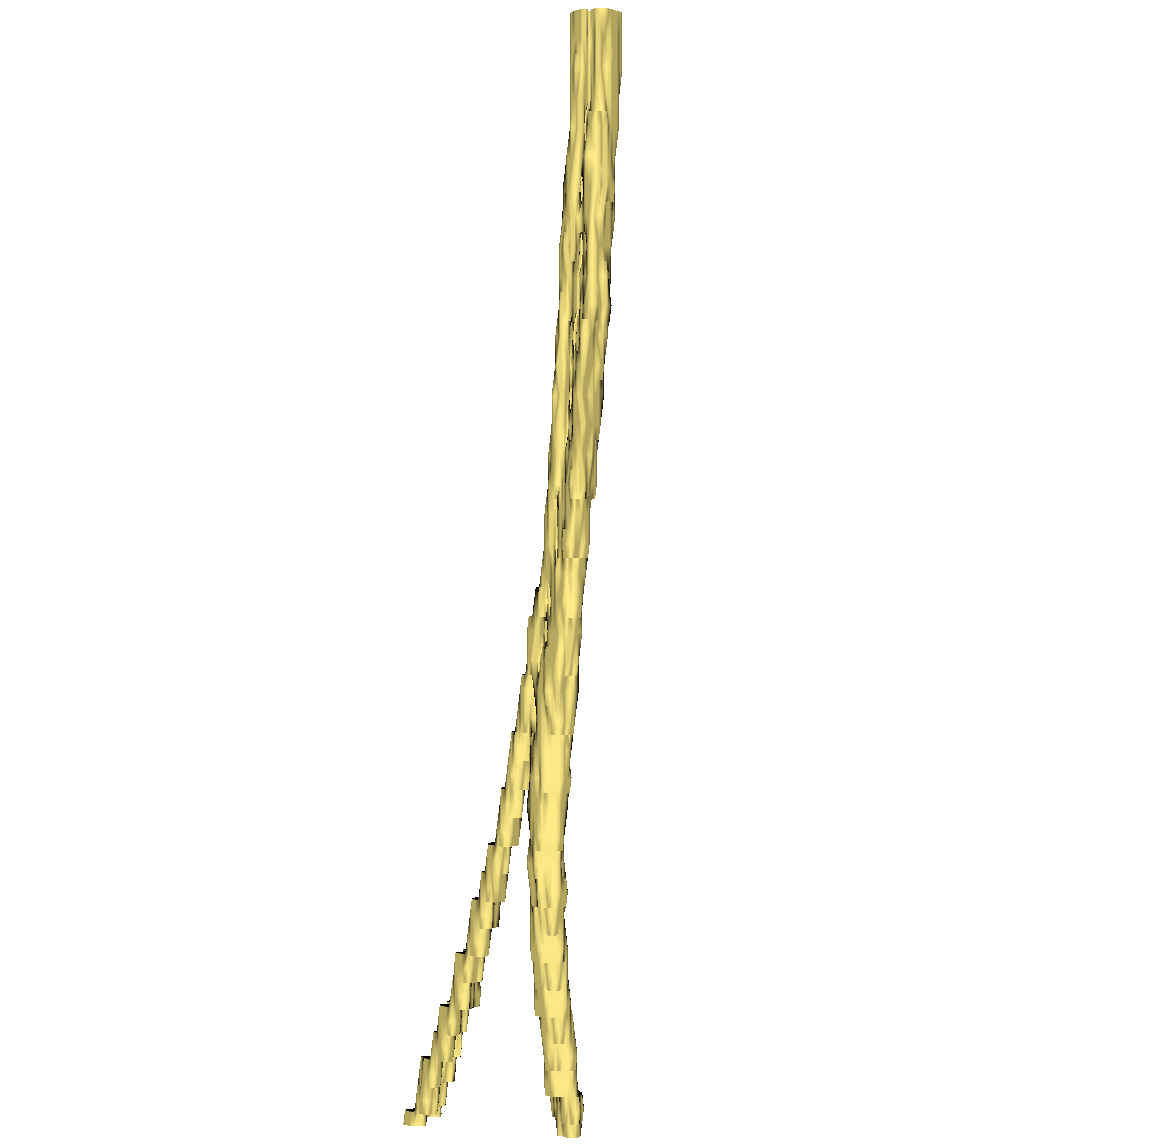
\includegraphics[width=\textwidth]{24A_gt_render}
    \caption[Ground Truth Rendering]{Anterior view of a 3D-rendering of the sciatic nerve based on the ground truth segmentation (rater OS). Clearly visible is the branching of the sciatic nerve into the tibial and fibular nerve.}
    \label{fig:gt_render}
\end{figure}

\begin{table}[htbp]
   \centering
   \caption[Descriptive Statistics of the Ground Truths]{The segmented ground truths with descriptive statistics of the voxel count and the mean sciatic nerve volume fraction.}
   \begin{tabular}{l*{6}{l}}
      \toprule
      Rater	& Cohort	& Mean		& SD		& Min		& Max		& Mean Volume	\\
      		&			& (voxels)	& (voxels)	& (voxels)	& (voxels)	& Fraction (\%)  \\
      \midrule
      OS  & Patient   & 13373.6 & 4602.1 & 7163.8 & 27428.4 & 0.155 \\
          & Volunteer & 5521.4  & 596.2  & 4615.6 & 6464.4  & 0.103 \\
      BW  & Patient   & 11519.1 & 5086.4 & 3691.7 & 30060.2 & 0.132 \\
          & Volunteer & 4686.8  & 676.1  & 4145.3 & 6299.7  & 0.088 \\
      LG  & Patient   & 12301.8 & 4035.2 & 4613.2 & 22526.4 & 0.142 \\
          & Volunteer & 5375.3  & 674.5  & 4342.2 & 6314.0  & 0.100 \\
      \midrule
	  GT  & Patient   & 11927.2 & 4240.6 & 5860.5 & 24845.5 & 0.138 \\
          & Volunteer & 5145.3  & 612.0  & 4458.0 & 6334.3  & 0.096 \\
      \bottomrule
   \end{tabular}
   \label{tab:ground_truths}
\end{table}


\subsection{Software \& Frameworks}
\subsubsection{Python}
Python\footnote{https://www.python.org/} (Python Software Foundation, Wilmington, DE, U.S.) is an interpreted high-level programming language which is widely used in academia and industry due to its effectiveness. Python is cross-platform and open-source. For all programming in this work we use Python version 3.6 together with (but not exclusively) the packages mentioned below.

\subsubsection{PyTorch}
PyTorch\footnote{https://pytorch.org/} (Facebook, Inc., Menlo Park, CA, U.S.) is a Python package for tensor computations with strong \gls{gpu} acceleration. Although at this point it is officially still in beta state, PyTorch has become an essential framework for deep learning research and applications with a rapidly growing community. We use PyTorch version 0.4.0 to implement and train the neural networks for this work.
\subsubsection{pymia}
The Python package pymia\footnote{https://pymia.readthedocs.io/} is developed and maintained by the \gls{mia} group at the \gls{istb}, University of Bern. The package contains generic and modular code for typical medical image analysis tasks. It offers lots of boilerplate code and we heavily relied on pymia to store, load, and transform the images as well as for the evaluation of the segmentation.
\subsubsection{ITK-SNAP}
ITK-SNAP\footnote{http://www.itksnap.org/} \cite{py06nimg} is an application for inspection and segmentation of medical images. The latest release of ITK-SNAP, version 3.6.0, was used to inspect the \gls{mrn} images, and to render and assess the ground truths and segmentations of the sciatic nerves.
\subsubsection{Seaborn}
Seaborn\footnote{https://seaborn.pydata.org/} is a statistical data visualization package for Python. We used Seaborn version 0.9.0 to analyze and plot our results.
\subsubsection{LibreOffice Calc}
LibreOffice Calc\footnote{https://www.libreoffice.org/} version 6.0.3.2 was used to create spreadsheets for the result tables.

\subsection{Hardware}
Training of the neural networks was done on the \gls{mia} group internal \gls{gpu} server. Most of the networks were trained on an NVIDIA Titan Xp. More demanding experiments, however, were trained on a NVIDIA Quadro P6000. Pre-processing, data augmentation and the calculation of the evaluation metrics were done using the \gls{cpu}. Post-processing was done on a desktop PC with an Intel Core i7 3.2 GHz \gls{cpu}, 64 GB memory and running Ubuntu 16.04 LTS.
\begin{table}[htbp]
   \centering
   \caption[Hardware]{Hardware overview of the \gls{mia} group \gls{gpu} server. \# corresponds to the number of cores or the number available of the respective \gls{gpu} type.}
   \begin{tabular}{l*{3}{r}}
      \toprule
      Property & Hardware & Memory / Frequency & \# \\
      \midrule
      \acrshort{cpu} & Intel Xeon E5-2620 & 2.10 GHz & 32 \\
      \acrshort{ram} & & 64 GB & \\
      GPU & NVIDIA 1080 Ti & 11 GB & 1 \\
       & NVIDIA Titan Xp & 12 GB & 5 \\
       & NVIDIA Quadro P6000 & 24 GB & 1 \\
      \bottomrule
   \end{tabular}
   \label{tab:cluster}
\end{table}

\section{Pre-processing} \label{sec:preprocessing}
Prep-rocessing is only applied to the \gls{mrn} image data of the \gls{ir} and T2 sequences. First, we registered the \gls{ir} image to the T2 image. Second, we normalized the intensities of the \gls{ir} and T2 images.\\
We registered the \gls{ir} image to the T2 image because of its lower in-plane resolution. We used a two step registration: i) rigid registration with three pyramid levels, and ii) affine registration with three pyramid levels. Mutual information~\cite{Maes1997MultimodalityInformation} was used as similarity metric. One setting of registration parameters was tuned for all cases heuristically by qualitative inspection of the registration results.\\
We intensity-normalized the \gls{mrn} images by subtracting the mean of each \gls{mrn} image and dividing by the standard deviation. This results in each \gls{mrn} case having an IR and T2 image with zero mean and unit variance. Input data normalization, as well as normalization in general, can be considered state-of-the-art and have been proven to be beneficial for training and performance of neural networks~\cite{Sola1997ImportanceProblems,SergeyIoffe2015BatchNormalization}.\\
Finally, the images are cropped to the correct input dimensions of the neural network during the data augmentation step, resulting in in-plane dimensions of $300 \times 300$, and $128 \times 128$ pixels respectively.


\section{Segmentation Pipeline}
Our segmentation pipeline has two phases: The training and the evaluation phase, depicted in Figures \ref{fig:pipeline} \textbf{A)} and \textbf{B)}, respectively. We use the pre-processed T2 and IR images together with the ground truth images to train the \gls{fcnn}. The trained \gls{fcnn} can then be used to segment the sciatic nerve from previously unseen (pre-processed) images. Finally, we apply post-processing to further leverage the segmenation accuracy.

The experiments in this thesis focused mainly on the network architectures, and the post-processing. The network architectures are described in Section \ref{sec:architecture} and the post-processing is described in Section~ \ref{sec:postprocessing}. Details to the training are given in the Section \ref{sec:training}.

\begin{figure}[htbp]
	\caption[Segmentation Pipeline]{Overview for the two phases of the whole segmentation pipeline: \textbf{A)} The FCNN is trained with the pre-processed and augmented T2, IR and ground-truth images. The optimizer adjusts the neural networks's weights based on a defined loss function. \textbf{B)} Once fully trained, the FCNN can segment the sciatic nerve on new images without the ground truth image. Finally, optional post-processing is applied.}
	\label{fig:pipeline}
	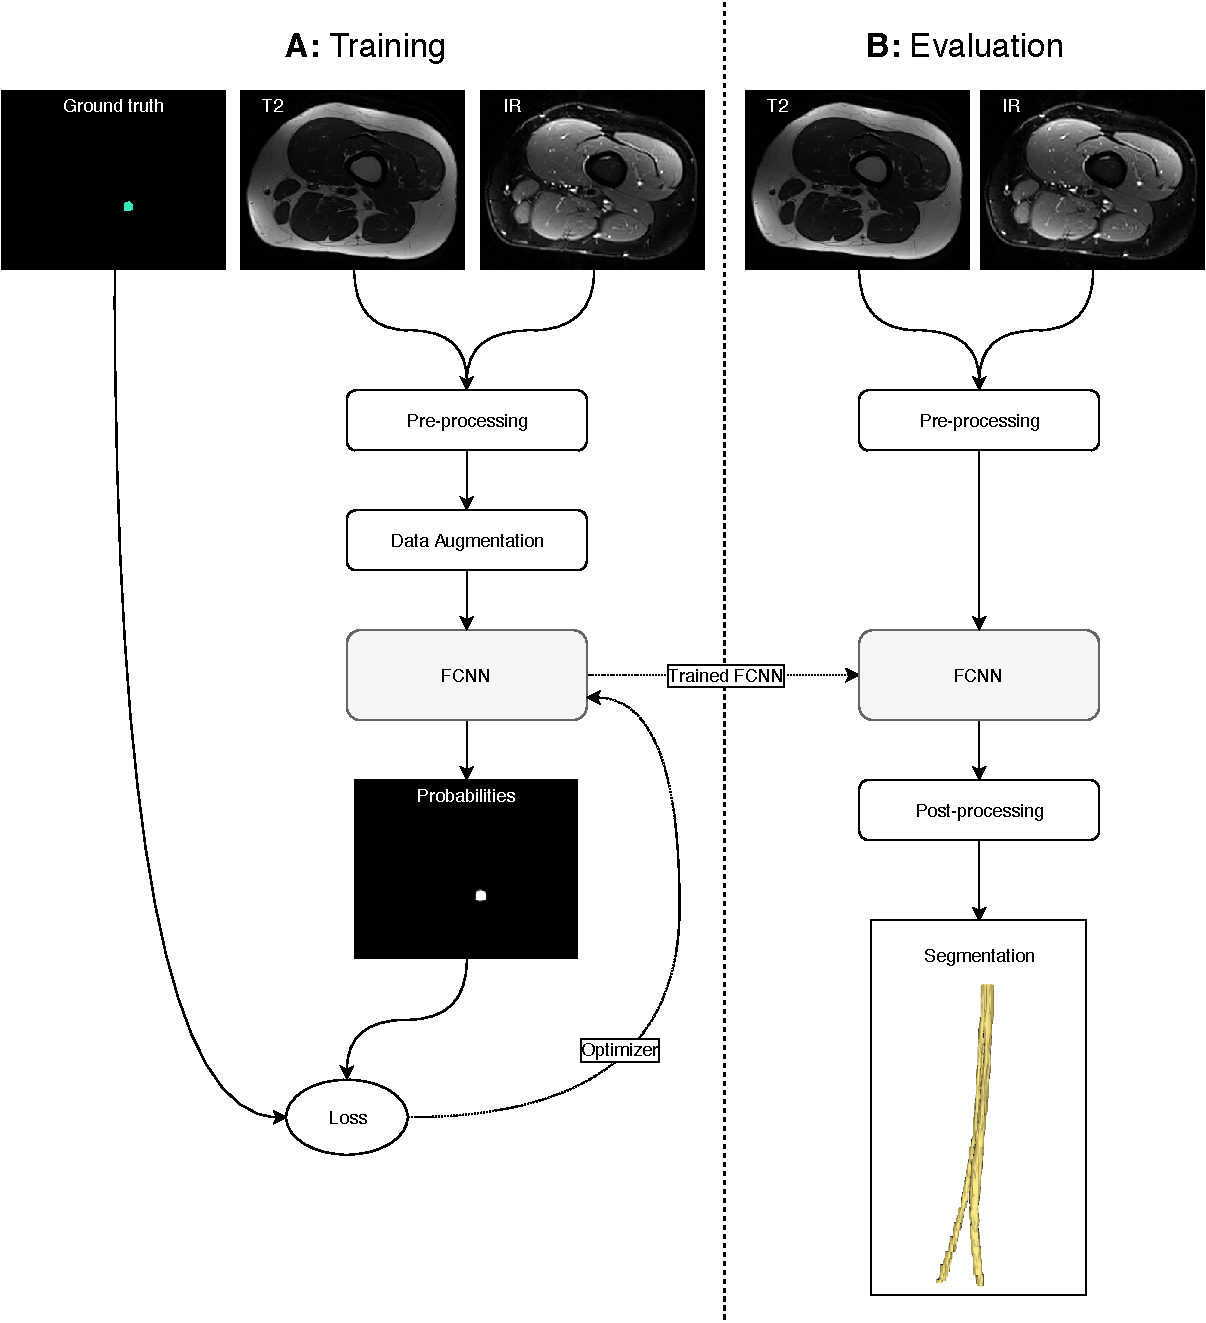
\includegraphics[width=\textwidth]{pipeline}    
\end{figure}

\section{Network Architectures} \label{sec:architecture}
We aim at investigating the optimal architecture and image input format for the segmentation tasks. Therefore, we selected a baseline architecture, which was incrementally changed based on our experiments and observations. As the baseline architecture we selected the U-Net by Ronneberger et al.~\cite{Ronneberger2015U-Net:Segmentation}. The U-Net architecture has proven to work well for semantic segmentation tasks and was originally developed for biomedical image segmentation.

All our \gls{fcnn}'s base on the encoder-decoder architecture of the U-Net, which is depicted in Figure~\ref{fig:unet}. We used a slightly modified version of the original paper based on the current state-of-the-art. We use dropout layers \cite{Srivastava2014Dropout:Overfitting} with probability $p = 0.2$, perform Batch Normalization \cite{SergeyIoffe2015BatchNormalization} and use the \gls{relu} activation function after each convolutional layer for all of our FCNN's. We always perform \textit{same}-padding and a stride of 1 for all convolutions, unless otherwise stated. Additionally we use 32 channels on the first encoder level, doubling the number on each down-transition in the encoder path of the architecture.
Similarly, in the decoder path, we reduce the number of channels by half after each up-transition. We want to segment the images voxels into the two classes \textit{background} and \textit{peripheral nerve}, respectively. This is a binary classification problem. Therefore the out-layer of all our neural networks consists of only one channel. We apply the sigmoid non-linearity to the out-layer to obtain the voxel-wise probability for peripheral nerve.\\
The chosen baseline architecture performs the segmentations on \gls{2d} images. Our \gls{mrn} images, however, are \gls{3d} images and the sciatic nerve is, none-the-less a 3D structure as well. We hypothesize that 3D-contextual information allows a neural network to create better nerve segmentations and therefore a \gls{3d} architecture should perform better than a \gls{2d} architecture. In order to investigate the impact of \gls{3d} information on the segmentation performance, we propose the following three network architectures:
\begin{enumerate}
  \item 2D Baseline
  \item 3D Stack-wise
  \item 3D Patch-wise
\end{enumerate}
The architectures have increasing access to the \gls{3d} information of the sciatic nerve, and are demonstrated in Figure~\ref{fig:inout} with respect to the image dimensions they take as input. The \gls{ir}, T2 and ground truth images are cropped to fit the respective input dimensions. During training phase, the cropping is performed randomly in the plane, as illustrated by Figure~\ref{fig:data_augmentation} and is part of data augmentation which is presented in Section \ref{sec:trainig:data_augmentation}. In the evaluation phase, the segmentations of the \gls{3d} images are performed by splitting the images, predicting and finally merging the prediction maps. These steps are all done based on the input and output dimensions of the respective architecture.

\begin{figure}[htbp]	
	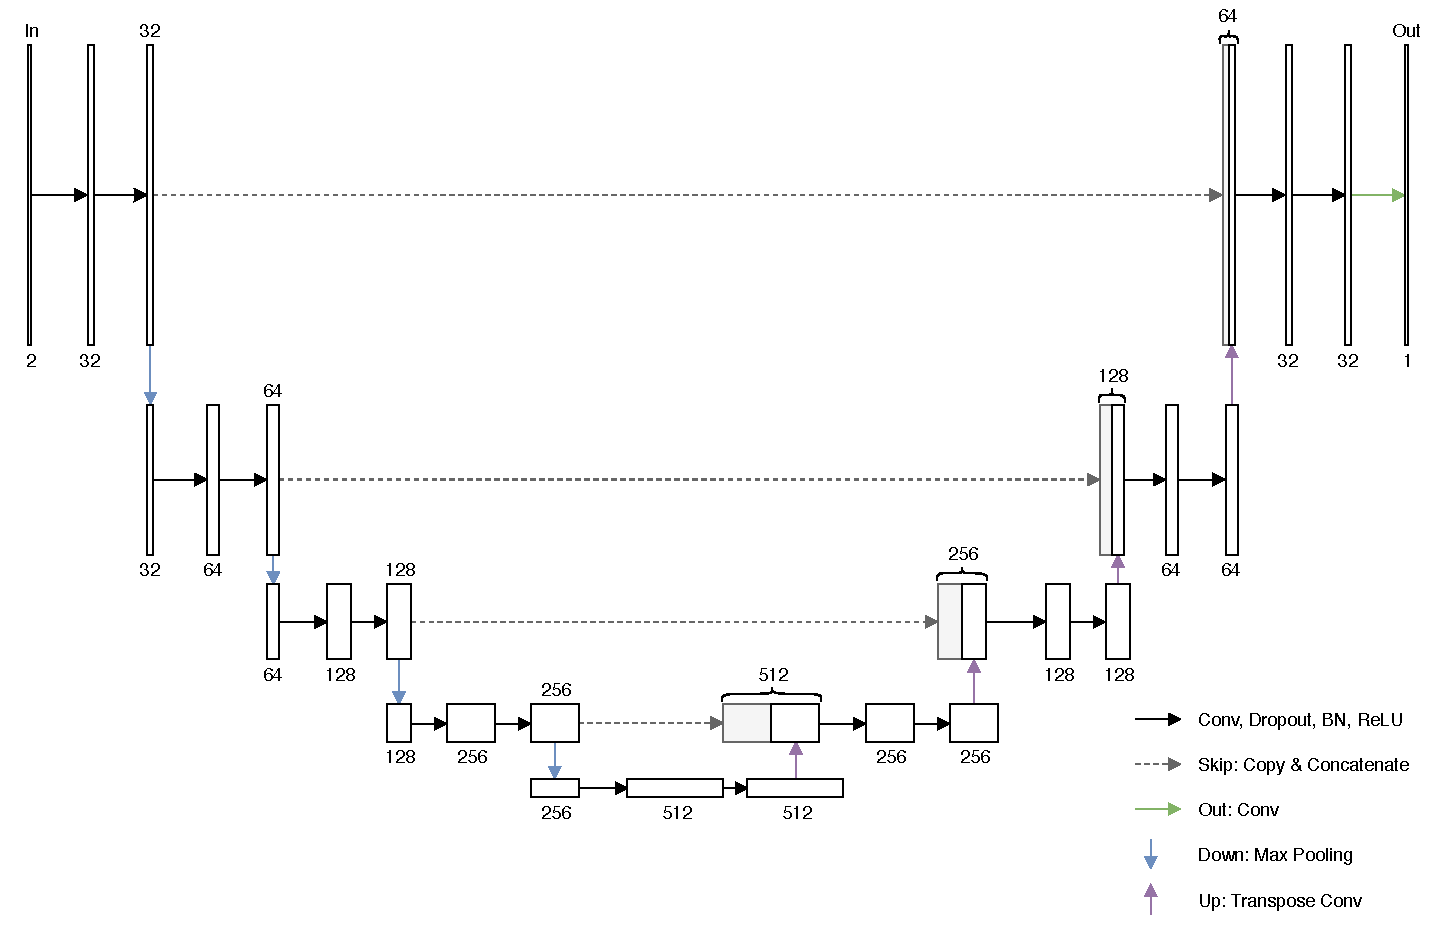
\includegraphics[width=\textwidth]{unet}
    \caption[Network Architecture]{The trained \gls{fcnn}s all implement an U-Net-like encoder-decoder architecture. The originally proposed U-Net has been extended by adding a dropout layer and performing \gls{bn} after each convolution layer. The numbers above and below the blocks indicate the number of channels. All convolutions are 3 $\times$ 3.}
    \label{fig:unet}
\end{figure}

\begin{figure}[htbp]
	\centering
	\subfloat[]
	{
		\label{fig:subfig:inout_base}
		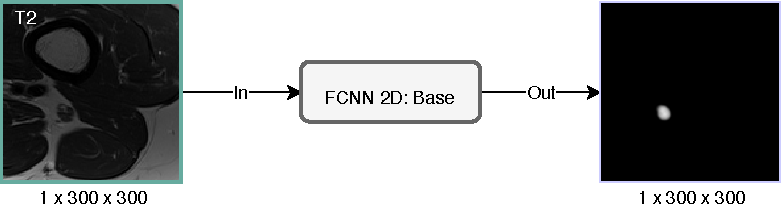
\includegraphics[width=\textwidth]{inout_base}
	}
	\hfill
	\subfloat[]
	{
		\label{fig:subfig:inout_stack}
		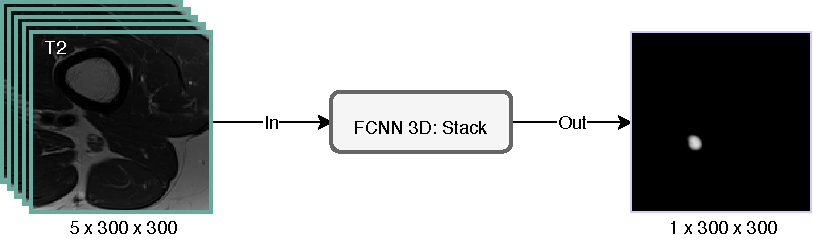
\includegraphics[width=\textwidth]{inout_stack}
	}
    \hfill
	\subfloat[]
	{
		\label{fig:subfig:inout_patch}
		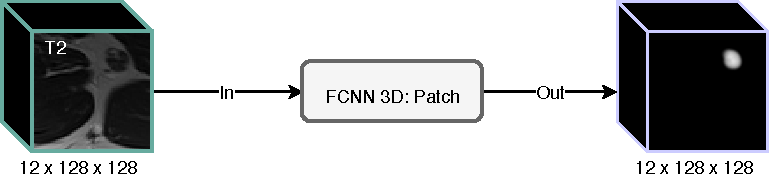
\includegraphics[width=\textwidth]{inout_patch}
	}
	\caption[Inputs and Outputs of the Architectures]{Depicted are the different input- and output dimensions (in axial, sagittal and coronal direction) for the proposed network architectures. Note, that for simplicity, only the T2 images are shown. The same dimensions apply to the \gls{ir} and ground truth images during the training phase. \textbf{a)} Baseline architecture which takes a single axial slice of $300 \times 300$ pixels as input, and outputs a single slice of probabilities of the same dimensions. The baseline architecture has no access to 3D information of the sciatic nerve at all and therefore is forced to learn \gls{2d} features only. \textbf{b)} The stack architecture receives multiple (5 in the case depicted) slices as input and makes predictions of either 1 or 3 axial slices, depending on the architecture. \textbf{c)} The patch architecture has access to more 3D information (12 slices) along the axial axis, but reduced access in-plane features due to its smaller in-plane resolution. The predictions of this architecture are of the same dimensions as the input.}
	\label{fig:inout}  
\end{figure}

\subsection{2D Baseline}
Our baseline architecture corresponds to the 2D U-Net as proposed by Ronneberger et al. \cite{Ronneberger2015U-Net:Segmentation} with dropout and Batch Normalization added. As mentioned before, we also start with 32 instead of 64 channels on the first encoder level. As Figure \ref{fig:subfig:inout_base} shows, the baseline architecture with its 2D kernels (3x3) handles 2D slices only, and therefore, has no access to 3D-contextual information. The details of the implemented architecture can be found in Table \ref{tab:architecture_fcnn_base} in the appendix.

\subsection{3D Stack-wise}
Driven by our hypothesis, we define an architecture which still closely resembles the baseline architecture, but has more access to the \gls{3d} information in the \gls{mrn} images.
We expand the \gls{2d} U-Net architecture to \gls{3d} by exchanging all building blocks (Convolutional layers, Max Pooling, Batch Normalization) with their \gls{3d} equivalent, similarly to Cicek et al.~\cite{Cicek20163DAnnotation}. In contrast to \cite{Cicek20163DAnnotation}, we keep the number of down- and up-sampling transitions and alternate between 2D kernels ($1 \times 3 \times 3$) and 3D kernels ($3 \times 3 \times 3$) within every level.
We feed this network multiple axial slices of $300 \times 300$ voxels as an input.
With the use of 3D kernels, and the multiple slices as input, the neural network can incorporate more of the 3D information to make predictions.
Details are to be found in in Table~\ref{tab:architecture_fcnn_volumetric} in the appendix. We trained the following versions of this architecture:
\begin{itemize}
  \item 3-to-1: 3 Input slices, prediction of 1 slice.
  \item 5-to-1: 5 Input slices, prediction of 1 slice.
  \item 5-to-3: 5 Input slices, prediction of 3 slices.
  \item 5-to-3: 5 Input slices, prediction of 3 slices. Projection-based loss function.
\end{itemize}
In essence, we feed the neural network the neighbouring slices (the previous two and next two in case of the 5-to-1 variant) to which it is supposed to make predictions about. We only predict fewer slices than the input slices because we expect to get better segmentation performance. The ability of the neural network to have access to all \gls{3d} information of the neighbouring slices should make it more confident about predictions on the slice(s) in the middle.
For the reason that our \gls{mrn} images have a much higher axial spacing (4.40 mm) as in-plane (0.52 mm) and also a lower axial resolution (30 to 60 slices) we decide to keep the up- and down-transitions in-plane and therefore do not perform pooling along the axial axis.\\
As test, and to further investigate the impact of \gls{3d} information we decided to train the 5-to-3 architecture and additional time with a experimental loss function based on projections: Instead of calculating the loss directly on the full $3 \times 300 \times 300$ voxels, we make a projection for each dimension (axial $300 \times 300$, sagittal $3 \times 300$ and coronal $3 \times 300$ pixels), normalize them and calculate the loss on each projection using the identically projected and normalized ground truth. Finally, we add the different loss terms together. Our motivation for this is the idea that the neural network should learn the projected shape of the nerve, which should be tube-like, and therefore possibly easier to learn.

\subsection{3D Patch-wise}
We increase the accessible 3D information along the axial axis even further by defining a network architecture similar to Cicek et al.~\cite{Cicek20163DAnnotation} featuring one up- and down-transition less than the other architectures. We conducted an experiment where we feeded the \gls{mrn} images to the neural network. We, however, were unable to successfully train the neural network and therefore decided to continue with a patch-based approach: We decrease the in-plane input dimensions to $128 \times 128$, and therefore reduce the accessible in-plane information for the network. We increase the number of slices fed to the network to 12. Furthermore the up- and down-transitions are only applied in the in-plane dimensions for the same reasons as mentioned for the stack-wise architecture. All the convolutional layers feature 3D kernels ($3 \times 3 \times 3$). The exact architecture is listed in Table~\ref{tab:architecture_fcnn_patches}.

\section{Training} \label{sec:training}
This section describes how we trained our neural networks and, therefore, corresponds to the steps depicted in Figure~\ref{fig:pipeline} \textbf{A)}. Once trained, a neural network is evaluated according to Section~\ref{sec:evaluation} and depicted in Figure~\ref{fig:pipeline} \textbf{B)}.

\subsection{Data Augmentation} \label{sec:trainig:data_augmentation}
A common problem during the training of neural networks is called overfitting. During training, the weights of the neural network get adjusted via the optimizer to reduce the loss on the training set. The primary goal of the training is to emphasize the neural network to learn meaningful features which generalize to previously unseen data, which is typically defined by the test set. 
Depending on the capacity of the neural network (its ability to fit a wide variety of functions, i.e. data \cite{Goodfellow2016DeepLearning}), the complexity of the task to solve, and the size of the training set, a neural network can start to overfit. If the neural network is somewhat complex, and training data is sparse, the neural network can begin to memorize the training examples rather than learning important features. This results in a high test-loss and hence a low performance on previously seen data, despite the training-loss being very low. Several counter-measures to overfitting exist, of which the most effective one is merely to use a bigger dataset. However, gathering and preparing a bigger dataset is time-consuming and often not possible, especially for medical images.\\
A possibility is to re-train the network in its capacity by reducing the numbers of convolutional layers or the number of features per convolutional layer.
Furthermore, there exist a variety of regularization techniques which may help:
$L^2$ (weight decay), $L^1$ (sparsity), early stopping \cite{Goodfellow2016DeepLearning}, dropout \cite{Srivastava2014Dropout:Overfitting}, and others.\\
One way to get around the problem of little annotated data is to create fake data and add it to the training set. This practice is known as data augmentation. Depending on the problem, the augmented data can be obtained either through transformation (e.g., cropping, flipping, mirroring, rotating) of existing training examples or can also be generated fully synthetically \cite{Tetteh2018DeepVesselNet:Volumes}.\\
We applied data augmentation by randomly transforming the data online during the training phase of the neural networks. We tested different sequences of transformations, including random crops, rotations, mirroring, elastic transformations and mixup, as proposed by Zhang et al.~\cite{Zhang2017Mixup:Minimization}, to prevent overfitting. In contrast to Eaton-Rosen et al.~\cite{Eaton-rosen2018ImprovingSegmentation}, mixup did not improve training or performance of the neural networks for us. The same was the case with the elastic distortions, so we decided not to use them. Figure \ref{fig:data_augmentation} shows the sequence of random transformation applied to each training sample before it was fed to the neural network during training: First, we randomly crop the input images (IR and T2) and the ground truth to the in-plane dimensions of $300 \times 300$ pixels. Second, we rotate the cropped images in-plane between 0 to 3 times randomly by 90\si{\degree}. Last, we mirror the images along the vertical edge in half of the cases.

\begin{figure}[htbp]	
	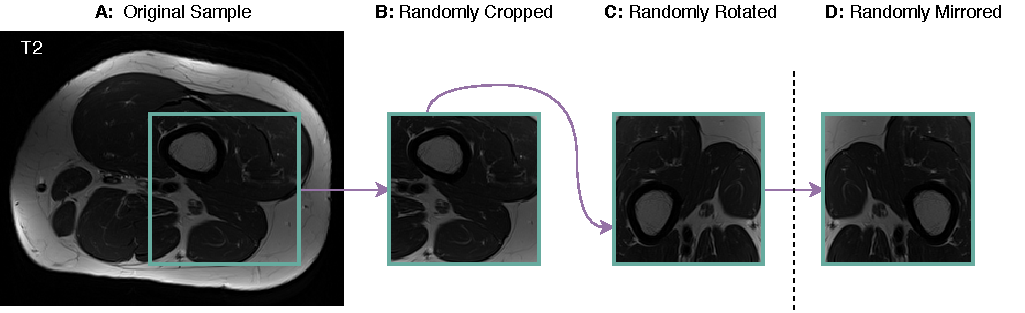
\includegraphics[width=\textwidth]{data_augmentation}
    \caption[Data Augmentation]{The sequence of random transformations applied to each training sample before feeding it to the neural network: \textbf{A)} The T2 image  before the data augmentation. \textbf{B)} Random crop to the dimensions $300 \times 300$. \textbf{C)} Rotation into a random direction. \textbf{D)} Mirroring with 50~\% probability. Note that the same transformation (per training sample) is applied to T2 image, IR image and ground truth, respectively. Furthermore, we also apply the same transformation to each slice for the neural networks which take multiple slices as input. }
    \label{fig:data_augmentation}
\end{figure}

\subsection{Loss Function}
We used the binary cross-entropy loss to train our neural networks. Due to the small amount of voxels belonging to the sciatic nerve (0.14\%) the segmentation task results in a highly imbalanced classification problem, with the \textit{background}-class, i.e. no sciatic nerve, being over 99 times more abundant than the \textit{sciatic-nerve}-class. This makes the training of the neural networks heavily biased towards background segmentation: In the beginning, the training loss can easily be reduced substantially by assigning all voxels to the \textit{background}-class. This is a common problem for medical image segmentation tasks with neural networks~\cite{Litjens2017AAnalysis,Tetteh2018DeepVesselNet:Volumes,Baumgartner2017AnSegmentation,Selvan2018ExtractionNetworks,Kayalibay2017CNN-basedData}\\
Buda et al.~\cite{BudaANetworks} systematically analyzed the impact of class imbalance on the classification performance on \acrshort{cnn}'s. They list and compare frequently applied solutions to this issue.\\
A solution to class imbalance is to use a weighted- or rebalancing loss. Ronneberger et al. \cite{Ronneberger2015U-Net:Segmentation} and Cicek et al.~\cite{Cicek20163DAnnotation} use a weighted cross-entropy loss to train their 2D and 3D U-Nets, respectively. Milletari et al.~\cite{Milletari2016V-Net:Segmentation} introduced a loss based on the Dice similarity coefficient, to account for the class imbalance. Several works, especially in the medical domain, successfully applied this loss or a variant of it \cite{Selvan2018ExtractionNetworks,Kayalibay2017CNN-basedData,Drozdzal2016TheSegmentation}. Sudre et al.~\cite{Sudre2017GeneralisedSegmentations} investigated the behaviour of weighted cross-entropy, sensitivity and Dice losses for their sensitivity to different rates of class imbalance in 2D and 3D segmentation tasks. They concluded that, depending on the imbalance rate, the use of the weighted or rebalancing losses help the optimization. Baumgartner et al.~\cite{Baumgartner2017AnSegmentation} compared cross-entropy, weighted cross-entropy and the Dice loss on different network architectures for cardiac MR image segmentation. They achieved superior performances with the cross-entropy losses (the weighted version being marginally better) and concluded, that for their task, the class imbalance was not a problem. They, however, reported a foreground prevalence of approximately 25 \% which is significantly higher than our prevalence of 0.14 \%.\\
Based on these results we conducted experiments with the baseline architecture to evaluate the benefit of weighted cross-entropy and Dice loss. Conversely to the results, we did not see any improvements during training or in the final performance when compared to unweighted cross-entropy loss. We, therefore, decided to use the binary cross-entropy loss for all our experiments. Additionally, we calculated and used the \acrlong{dice} in conjunction with the training and test losses to monitor the training progress.

\subsection{Optimizer}
We use PyTorch's implementation of the Adam optimizer \cite{Kingma2014Adam:Optimization} without weight decay, $\beta_1 = 0.900$, and $\beta_2 = 0.999$ for the training of all networks. A listing of all hyperparameters can be found in Table~\ref{tab:hyperparameters} in the appendix.

\section{Post-processing} \label{sec:postprocessing}
\begin{figure}[htbp]
    \centering
	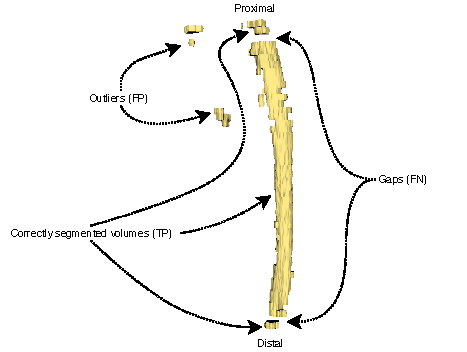
\includegraphics[width=\textwidth]{fpfn}
    \caption[Segmentation Issues]{First results showed that the unprocessed segmentations were typically corrupted by false positive (FP) outliers and false negatives (FN) visible as gaps. While the outliers impact the distance metrics, i.e. \gls{hd}, the gaps make post-processing harder: Simply keeping the largest volume present, would remove all smaller correctly segmented volumes (TP).}
    \label{fig:fpfn}
\end{figure}
Early experiments showed that there are \gls{fp} outliers as well as \gls{fn} discontinuities present in the segmentations, see Figure~\ref{fig:post_processing}. The distance metrics, especially the \acrshort{hd}, are sensitive to these (\acrshort{fp}). The (\acrshort{fp}) outliers all tend to have small volumes and therefore could easily be removed by keeping only the largest volume present in the segmentation. The presence of (\acrshort{fn}), visible as gaps, however, makes this a more difficult task: They split the nerve into multiple correctly segmented volumes (\acrshort{tp}). Simple and naive post-processing by keeping only the largest volume, would also remove all smaller correctly segmented volumes.\\
With the aim to increase the quality of sciatic nerve segmentations by reducing the (\acrshort{fp}), we apply the two following post-processing steps to the output of a neural network: First, we try to connect the correctly segmented volumes to form one large volume. Second, we only keep the largest volume.\\
\begin{figure}[htbp]	
	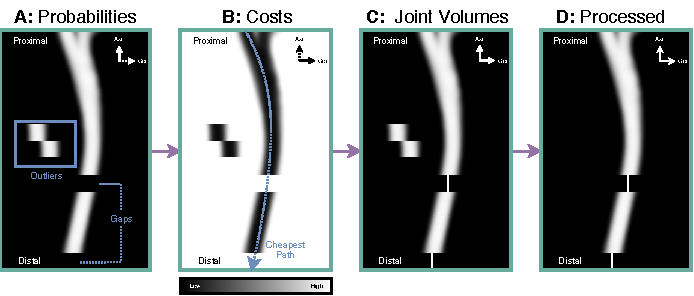
\includegraphics[width=\textwidth]{post_processing}
    \caption[Post-processing]{Post-processing steps applied ot the output of a neural network to increase segmentation performance. \textbf{A)} Output of the neural network corrupted by outliers (FP) and gaps (FN). \textbf{B)} Costs for the calculation of the cheapest path. Costs are obtained by taking the background probabilities ($p_{background} = 1 - p_{nerve}$) for each voxel. Cheapest path is along the (TP) volumes. \textbf{C)} All voxels along the cheapest path are labelled as nerve, merging the (TP) volumes to one big volume. \textbf{D)} All but the biggest volume are removed, resulting in fewer (FP).}
    \label{fig:post_processing}
\end{figure}
Given the anatomy of the sciatic nerve and the anatomical region the MRN images were taken from, we know it passes through both, the most proximal and distal slice. Additionally, we know that all (\acrshort{tp}) lie on a long tubular-like path along the cario-caudal axis given by the anatomy of the sciatic nerve. Once we know the path, we can use it to connect the (\acrshort{tp}) volumes.\\
We treat this as a directed graph problem, where we want to find the cheapest path from the most proximal to the most distal slice. The intermediate steps are depicted in Figure~\ref{fig:post_processing}: \textbf{A)} The predictions of the neural networks can be corrupted by (\acrshort{fp}) and (\acrshort{fn}). \textbf{B)} Therefore, we define the voxels of the probability image to be the graph nodes, with each having a cost of the inverse of the sciatic nerve probability to pass through. Therefore, voxels with high probability being peripehral nerve are cheap and hence favourable candidates to be part of the cheapest path. To find the cheapest path through the graph we make use of Dijkstra's Algorithm~\cite{Dijkstra1959AGraphs}. \textbf{C)} Once the cheapest path is found, we label all voxels on the path to belong to the sciatic nerve. This step joins all (TP) volumes on the path to form one large connected component. \textbf{D)} After we merged all (TP) to one volume, we only keep the largest component/volume.

\section{Evaluation} \label{sec:evaluation}
This section describes how we evaluate our neural networks after the training phase. Section~\ref{sec:eval_cross} explains the evaluation scheme we apply. In Section~\ref{sec:eval_metrics} our evaluation metrics are presented and Section~\ref{sec:eval_strategy} describes how we deal with the fact that our neural networks have other input dimensions than the dimensions of our \gls{mrn} images.

\subsection{Cross-validation} \label{sec:eval_cross}
In deep learning, evaluation of a model is typically done by \gls{lpocv}: $p$ samples are left out from the dataset to form a training set and validation set of sizes $|S_{train}| = n - p$ and $|S_{valid}| = p$, respectively. As the name implies, the model is trained on the training set. The validation set is used to validate and tune the hyperparameters of the model.
Depending on the dataset size, the split is done randomly or in a semi-random fashion to ensure that the subsets have the same distribution of samples.
A good practice is to split the dataset in the same manner into three subsets, namely the training, validation and test set. Typical values for the split fractions could be 0.7, 0.1 and 0.2 for training-, validation- and test-set respectively. As no data of the test set is used for training or tuning the model, the test set allows evaluating the metrics (Section~\ref{sec:eval_metrics}) on unseen data. \\
The split of the dataset into three separate subsets with similar sample distribution is, however, not always possible, especially if dataset sizes are small. In such cases, evaluation with a \gls{kfcv} may be more a more practical choice: The dataset is split into $k$ equal sized folds, still aiming to have similar sample distributions. Sequentially, one of the folds is left out and used as a validation set, while the model is trained on all of the remaining folds. An approximate accuracy and performance on unseen data can be obtained by averaging the results of the evaluation metrics calculated on the $k$ validation folds.\\
As the size of our dataset (n = 52) is comparably small to other datasets we chose to validate our models via four-fold cross-validation, i.e. our models are trained on 39 subjects and evaluated on 13 subjects. We randomly assigned the patient subjects to the folds but with stratification regarding the volunteers. I.e. we ensured that the volunteers are equally distributed. The assignment of the subjects is summarized in the Table \ref{tab:fold_assignment}. We trained and tuned the neural networks only using the reported semi-random assignment. We did not use any other assignment to develop the method.

\subsection{Metrics} \label{sec:eval_metrics}
To measure and assess the performance of a neural network, evaluation metrics are required. The metrics are calculated by comparison of the segmentation mask (the output of a neural network) to the ground truth obtained by majority voting of the manual expert segmenations. Taha and Hanbury~\cite{Taha2015MetricsTool} analyzed popular metrics for 3D medical image segmentation and provided metric selection guidelines. Based on the guidelines, we choose the following evaluation metrics, and report their mean and \gls{sd} in Chapter~\ref{chap:results}.

\begin{itemize}
\item \acrlong{dice}:
  \begin{itemize}
  \item Outliers are to be expected.
  \item De-facto gold standard.
  \end{itemize}
\item \acrlong{vs}
  \begin{itemize}
  \item Good nerve volume agreement is of clinical interest.
  \end{itemize}
\item \acrlong{avd}
  \begin{itemize}
  \item Sciatic nerve segmentations satisfy conditions for small segments.
  \item Low sensitivity to outliers.
  \end{itemize}
\item \acrlong{hd95}
  \begin{itemize}
  \item Sciatic nerve segmentations satisfy conditions for small segments.
  \item Low sensitivity to outliers
  \item Comparison to publications.
  \end{itemize}
\item \acrlong{hd}
  \begin{itemize}
  \item Sciatic nerve segmentations satisfy conditions for small segments.
  \item We want to analyze the impact of our Post-processing
  \item Comparison to publications.
  \end{itemize}
\end{itemize}

Let $S \in \{0, 1\}$ be the output segmentation mask of a model and $G \in \{0, 1\}$ be the ground truth.
$S_{1}$ denotes the set of all voxels where $S = 1$, i.e., where the neural network detected the foreground. Analogously, $G_{1}$ denotes the set of all voxels where $G = 1$. The number of all voxels in a set $A$ is denoted by the cardinality operator $|A|$.

\subsubsection{\acrlong{dice}}
The \gls{dice} \cite{Dice1945MeasuresTh} is an overlap metric defined as the following:
\begin{equation}
   DICE(S, G) \in [0, 1] = \frac{2|S_{1} \cap G_{1}|}{|S_{1}| + |G_{1}|}.
   \label{eq:dice}
\end{equation}
The \gls{dice} is the most used metric for validating medical image segmentations \cite{Taha2015MetricsTool}. A \gls{dice} value of $1.0$ corresponds to a perfect volumetric overlap of the neural networks foreground segmentation and the ground truth. Important to mention is that the significance of the \gls{dice} drops with increasing volume fraction of the foreground. For instance, a ground truth with a foreground volume fraction of 50\% and a randomly initialized segmentation mask lead to a \gls{dice} of $0.5$. Consequently, the \gls{dice} is much more meaningful in the case of a low volume fraction of the foreground. The fact that the sciatic nerve only accounts for about 0.14\% of the voxels makes this metric well suited for our problem. This, however, means also that we are generally obtaining lower \gls{dice} coefficients which has to be considered when we make comparisons to other segmentation problems with higher foreground prevalence.

\subsubsection{\acrlong{vs}}
The \gls{vs} \cite{Taha2015MetricsTool} is, as the name implies, a volume-based metric. The \gls{vs} can be defined in terms of the \gls{vd} as $1 - \acrshort{vd}$. That is
\begin{equation}
   VS(S, G) \in [0, 1] = 1 - \frac{||S_{1}| - |G_{1}||}{|S_{1}| + |G_{1}|}.
   \label{eq:vs}
\end{equation}
As \gls{vs} is only considering the volumes, the metric does not allow any inference on the alignment or agreement of the shapes of the compared segmentations. This means two segmentations with no overlap at all, consequently with a \gls{dice} of zero, can still result in a high \gls{vs} or even have the same VS, i.e. a VS of 1. In contrary, a high \gls{dice} will always result in a high \gls{vs} because the \gls{vs} is directly correlated to the \gls{dice}.

\subsubsection{\acrlong{hd}}
The \gls{hd} is a distance metric between two sets $S$ and $G$ defined by
\begin{equation}
   HD(S, G) = \max(d_{H}(S,G),d_{H}(G,S)),
   \label{eq:hd}
\end{equation}
where $d_{H}(S,G)$ is the directed \gls{hd} that is given by
\begin{equation}
   d_{H}(S, G) = \max\limits_{s \in S} \min\limits_{g \in G} ||s-g||,
   \label{eq:dhd}
\end{equation}
where $||s-g||$ is some norm, e.g. the Euclidean distance. The \gls{hd} is generally susceptible to outliers, which we have present in the outputs of the neural networks in form of false-positively segmented regions. It is therefore not recommended to directly use the \acrshort{hd} \cite{Taha2015MetricsTool}. Instead, Huttenlocher et al. \cite{Huttenlocher1993ComparingDistance} proposed to use the \gls{hd95}, which is less outlier sensitive. We will report both, \gls{hd} and the \gls{hd95} to be able to compare the metrics.

\subsubsection{\acrlong{avd}}
The \gls{avd}, also known as the average \gls{hd}, is the \gls{hd} averaged over all distances. It is stable and less sensitive to outliers when compared to the \gls{hd}, and also less sensitive than the HD95~\cite{Taha2015MetricsTool}. The \gls{avd} is defined by
\begin{equation}
   AVD(S, G) = \max(d_{AH}(S,G),d_{AH}(G,S)),
   \label{eq:avd}
\end{equation}
where $d_{AH}(S,G)$ is the directed average \gls{hd} that is given by
\begin{equation}
   d_{AH}(S, G) = \frac{1}{N} \sum\limits_{s \in S} \min\limits_{g \in G} ||s-g||.
   \label{eq:dahd}
\end{equation}

\subsection{Baseline} \label{sec:eval_baseline}
We compare and evaluate the performance of our method to the consensus ground truth GT and to the inter-rater variability, which serves us as a final performance baseline. We obtain the inter-rater variability by calculating our evaluation metrics for each rater-rater pair using the corresponding ground truth segmentation. Hence, the inter-rater variability for each metric consists of $n = 126$ and $n = 30$ for the patient and volunteer cohort, respectively.

\subsection{Strategy} \label{sec:eval_strategy}
Our neural networks have smaller input dimensions than the typical size of the \gls{mrn} images ($60 \times 330 \times 384$). We need, therefore, to split the \gls{mrn} images into junks of the respective input dimensions during the evaluation phase. The junks are then fed sequentially to the neural network, and the obtained probability maps are combined to form a segmentation of the whole volume. We do the splitting and combination slice-wise for the baseline and stack-wise architectures. We crop the slices centrally to an in-plane resolution of $300 \times 300$ voxels to fit the input dimensions of the architectures. The sciatic nerves, generally located central in the transverse plane, lie within the cropped images. No cropping is needed in the case of the patch-wise architecture: The whole image is split into $12 \times 128 \times 128$ volume patches, predicted, and recombined to form the segmentation. The process of dividing, predicting and combining the \gls{mrn} images is explained in Figure~\ref{fig:eval_strategy} in more detail.

\begin{figure}[htbp]
	\centering
	\subfloat[]
	{
		\label{fig:subfig:eval_stack}
		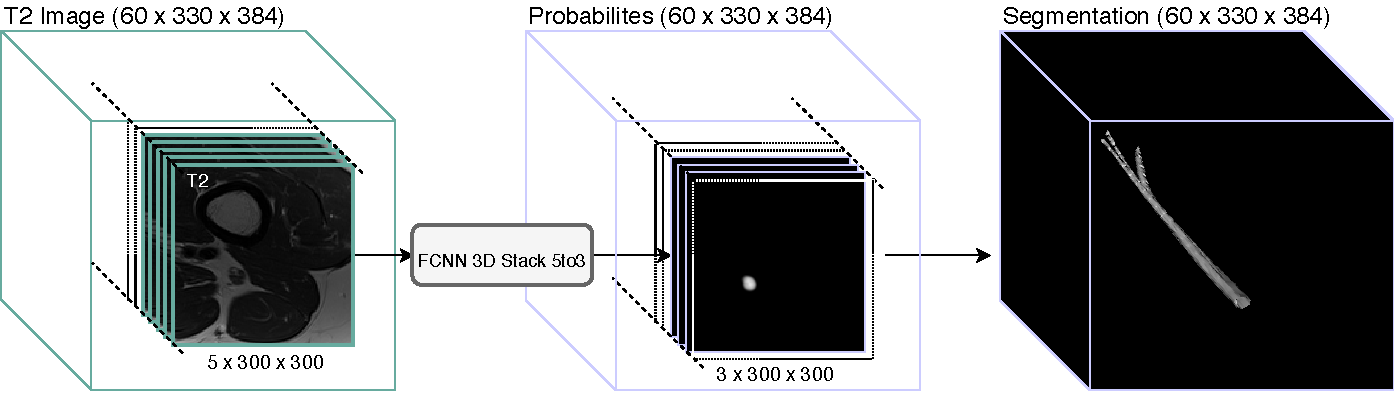
\includegraphics[width=\textwidth]{eval_stack}
	}
	\hfill
	\subfloat[]
	{
		\label{fig:subfig:eval_patch}
		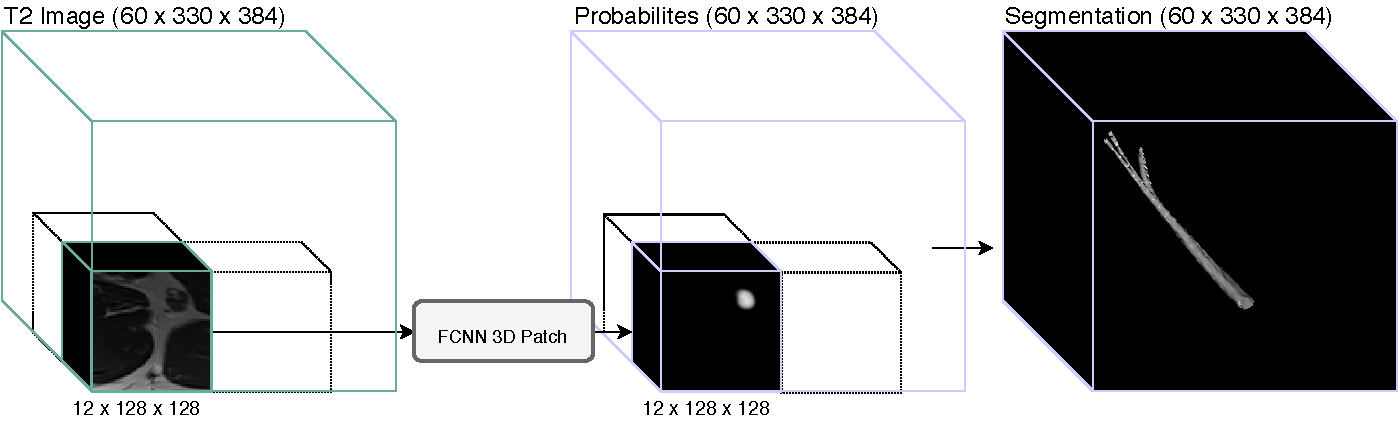
\includegraphics[width=\textwidth]{eval_patch}
	}
	\caption[Evaluation Strategy]{In the evaluation phase, a segmentation with the same dimensions as the ground truth is required from the trained neural network. In order to obtain the segmentation, the image is split into (stacks of) slices or volumes and fed to the neural network. The probability maps, which are the output of the network, are stitched together yielding a probability map of the whole volume. Simple thresholding of the probabilities results in the segmentation, which in return is used to calculate the evaluation metrics upon, together with the ground truth. \textbf{a)} The evaluation for the baseline and stack-wise architectures is done slice-wise: All slices are cropped centrally to an in-plane resolution of $300 \times 300$ voxels and fed sequentially to the neural network (in blocks of 3 or 5 for the stack-wise architecture). The resulting probability maps are concatenated, thresholded and symmetrically padded back up to the input/ground truth dimensions \textbf{b)} To get the segmentation of the patch-architecture, the input image is split into multiple $12 \times 128 \times 128$ patches. The patches are fed to the network sequentially yielding probability patches. These are combined and thresholded to obtain the segmentation.}
	\label{fig:eval_strategy}  
\end{figure}



\section{Experiments} \label{sec:experiments}
We propose the following experiments to validate our hypothesis:\\

\textit{Experiment 1:} We train and evaluate the baseline architecture on our \gls{mrn} images to investigate whether a deep learning-based approach for fully-automatic peripheral nerve segmentation is feasible. We evaluate the performance only to the consensus ground truth.

\textit{Experiment 2:} Driven by the hypothesis that \gls{3d} context allows for better segmentation results, we train and evaluate the stack-wise and patch-wise architectures on our \gls{mrn} images and compare their performance to the segmentation performance of the baseline architecture. We do not apply post-processing. We evaluate the performance only to the consensus ground truth.

\textit{Experiment 3:} We take our best performing architecture and compare the segmentation performance with and without post-processing applied. We evaluate the performance only to the consensus ground truth.

Finally, we take the best performing combination of architecture and post-processing of the experiments and compare the performance to the inter-rater variability.

\endinput
\chapter{Results} \label{chap:results}
In this chapter, the obtained results from the defined experiments in Section~\ref{sec:experiments} are presented. In Section~\ref{sec:exp_feas} we summarize the results for the feasibility of deep learning-based peripheral nerve segmentation.
Section~\ref{sec:exp_3dcontext} presents the performances for the different neural network architectures with variable access to \gls{3d} information.
In Section~\ref{sec:exp_pp} presents the impact of post-processing applied to the segmentation of the baseline architecture and the best performing \gls{3d} architecture, respectively.
Finally, Section~\ref{sec:exp_evaluation} features the results obtained concerning the inter-rater variability, to which we compared and evaluated our best performing method.
The detailed results of the individual experiments can be found in the Appendix~\ref{app:results}.

\section{Experiment 1: Feasibility} \label{sec:exp_feas} %=======================================================
We successfully trained the baseline architecture on the \gls{mrn} images. In order to gain insight in the importance of the two input images (T2 and \gls{ir}), we trained the baseline architecture three times: once on each image separately, and once with both images. The mean and \gls{sd} for each of the training runs are summarized in Table~\ref{tab:results_feasibility}. Figure~\ref{fig:results_boxplot_T2_IR_dice} features a boxplot for the \acrlong{dice}. The results show that the training on both images yields the highest scores for all metrics except the \acrlong{vs} for the volunteer cohort. Training using only the T2 image results in comparable results as when trained with both images, concerning the \gls{dice} and \gls{vs} metrics. However, training using only the T2 image resulted in a significantly higher \gls{hd95} when compared to training on both images. Based on these results, we decided to use both images for all further training. The training took approximately 3 hours on a NVIDIA Titan Xp independent of the input. Testing a single \gls{mrn} case, hence segmenting it, took less than 3 seconds.

\begin{table}[htbp]
   \centering
   \caption[Results for Feasibility]{Mean and \gls{sd} of the \acrlong{dice}, \acrlong{vs}, and \acrlong{hd95}. The baseline was trained and evaluated on T2-only, IR-only and on the combination of them (T2 and IR).}
   \begin{tabular}{l*{4}{l}}
      \toprule
      Cohort	& Image  & DICE              & VS				& HD95\\
      			&			&					&					& (mm)\\
      \midrule
      Patient   & T2 and IR & $\mathbf{0.704 \pm 0.139}$& $\mathbf{0.882 \pm 0.098}$ & $\mathbf{16.526 \pm 17.025}$ \\
                & T2        & $0.695 \pm 0.142 $& $0.879 \pm 0.111$ & $ 17.522 \pm 17.218$ \\
                & IR        & $0.384 \pm 0.197 $& $0.733 \pm 0.226$ & $ 23.124 \pm 17.229$ \\
      \midrule
      Volunteer & T2 and IR & $\mathbf{0.861 \pm 0.057 }$& $0.921 \pm 0.056$ & $\mathbf{1.644 \pm 2.321}$ \\
                & T2        & $0.840 \pm 0.078 $& $\mathbf{0.936 \pm 0.054}$ & $ 5.909 \pm 12.433$ \\
                & IR        & $0.648 \pm 0.097 $& $0.900 \pm 0.114$ & $ 11.974 \pm 16.394$ \\
      \bottomrule
   \end{tabular}
   \label{tab:results_feasibility}
\end{table}

\begin{figure}[htbp]
	\centering
	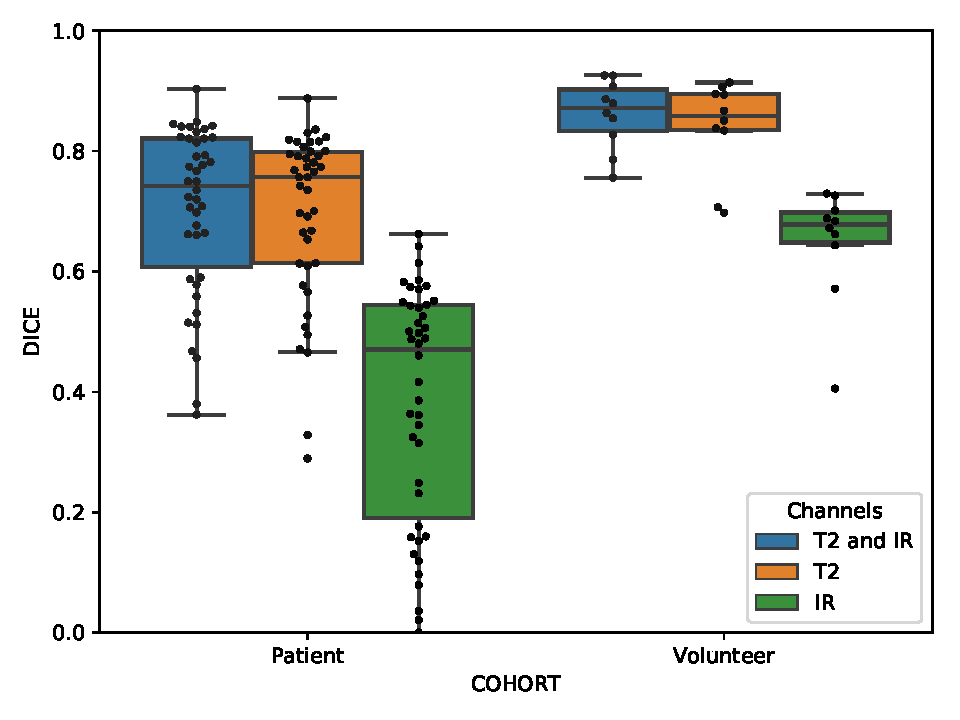
\includegraphics[width=0.8\textwidth]{boxplot_T2_IR_DICE}
    \caption[Boxplot of the \acrlong{dice} for the baseline architecture]{Boxplot of the \acrlong{dice} for the baseline architecture trained on T2 and IR, T2-only, and IR-only. Note that comparable segmentation performance is achieved by only using the T2 image. Using only the IR channel, however, results in a significantly lower performance.}
    \label{fig:results_boxplot_T2_IR_dice}
\end{figure}

\section{Experiment 2: 3-D Context} \label{sec:exp_3dcontext} % ==================================================
We successfully trained the neural networks with the proposed \gls{3d} architectures, which enables incorporating more \gls{3d} context information. The mean and \gls{sd} for the \acrlong{dice}, \acrlong{vs}, and \acrlong{hd95} are summarized in Table~\ref{tab:results_3d_context_small} together with the baseline results. A boxplot for the \acrlong{dice} is shown in Figure~\ref{fig:results_boxplot_dice}. The stack-based method achieved almost constantly better results than the baseline. The projection-based and patch-based architectures resulted in worse performance. Figure~\ref{fig:results_heatmap_dice} features a heatmap, listing the achieved \acrlong{dice}s on the patients and volunteers for all neural network architectures. The heatmap reveals that the lowest \gls{dice} values are achieved mostly on patient subjects, independent of the network architecture. Some of the outliers in the Boxplot~\ref{fig:results_boxplot_dice} are due these low \gls{dice} values. Training took 15 and 22 hours on a NVIDIA Titan Xp for the stack-wise and patch-wise neural networks, respectively. Testing a single \gls{mrn} case took less than 3 seconds. The complete results, also featuring the \acrlong{avd} and \acrlong{hd}, can be found in the appendix Table~\ref{tab:results_3d_context}.

\begin{table}[htbp]
   \centering
   \caption[Results for 3-D Context]{Mean and \gls{sd} of the \acrlong{dice}, \acrlong{vs}, and \acrlong{hd95} for different \gls{3d} context information.}
   \begin{tabular}{l*{6}{l}}
      \toprule
      Cohort	& Architecture	& DICE				& VS				& HD95\\
      			&					&					&					& (mm)\\
      \midrule
      Patient   & 2-D baseline & $0.704 \pm 0.139$ & $0.882 \pm 0.098$ & $16.526 \pm 17.025$ \\
                & Stack\_3to1  & $0.749 \pm 0.139$ & $0.896 \pm 0.123$ & $\mathbf{10.807 \pm 13.393}$ \\
                & Stack\_5to1  & $\mathbf{0.765 \pm 0.123}$ & $\mathbf{0.898 \pm 0.110}$ & $12.418 \pm 19.104$ \\
                & Stack\_5to3  & $0.717 \pm 0.135$ & $0.883 \pm 0.105$ & $19.312 \pm 22.545$ \\
                & Stack\_Proj  & $0.712 \pm 0.136$ & $0.889 \pm 0.094$ & $19.878 \pm 21.613$ \\
                & Patch & $0.682 \pm 0.128$ & $0.876 \pm 0.101$ & $24.241 \pm 20.896$ \\                
      \midrule
      Volunteer & 2-D baseline & $0.861 \pm 0.057$ & $0.921 \pm 0.056$ & $1.644  \pm 2.321 $ \\
                & Stack\_3to1  & $0.860 \pm 0.073$ & $0.925 \pm 0.043$ & $2.260  \pm 2.336 $ \\
                & Stack\_5to1  & $\mathbf{0.878 \pm 0.048}$ & $\mathbf{0.928 \pm 0.048}$ & $1.537  \pm 1.784 $ \\
                & Stack\_5to3  & $0.855 \pm 0.052$ & $0.928 \pm 0.062$ & $\mathbf{1.350  \pm 1.365} $ \\                
                & Stack\_Proj  & $0.842 \pm 0.051$ & $0.917 \pm 0.067$ & $1.642  \pm 1.549 $ \\
                & Patch & $0.806 \pm 0.068$ & $0.888 \pm 0.085$ & $7.992  \pm 13.474$ \\
      \bottomrule
   \end{tabular}
   \label{tab:results_3d_context_small}
\end{table}

\begin{figure}[htbp]
	\centering
	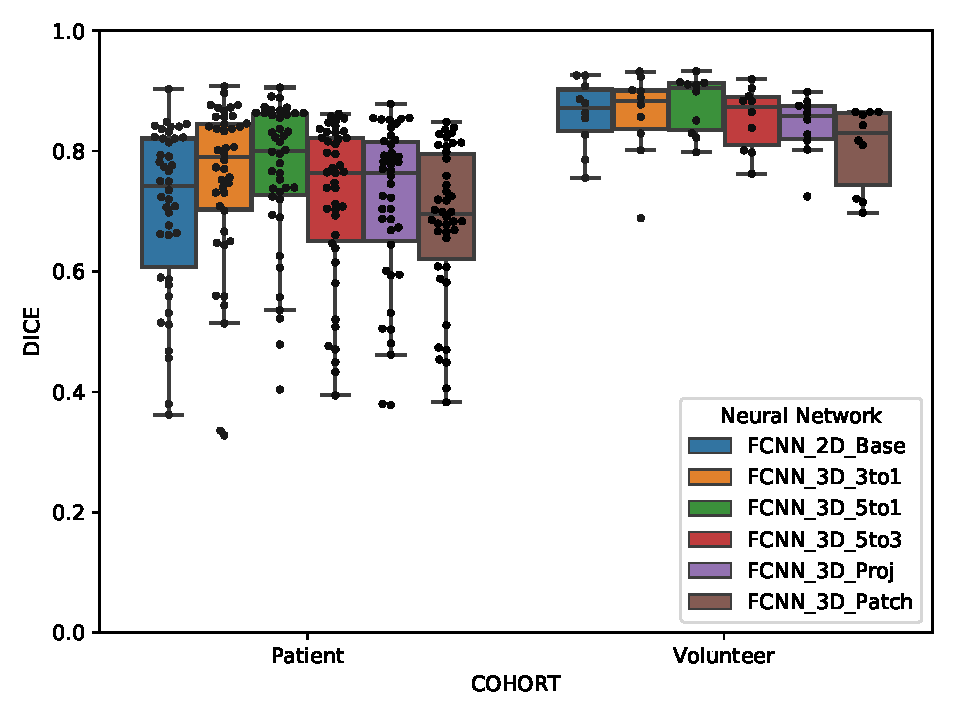
\includegraphics[width=\textwidth]{boxplot_DICE}
    \caption[Boxplot of the \acrlong{dice} for 3-D context architectures]{Boxplot of the \acrlong{dice} for the different \gls{3d} context architectures.}
    \label{fig:results_boxplot_dice}
\end{figure}

\begin{figure}[htbp]	
	\centering
	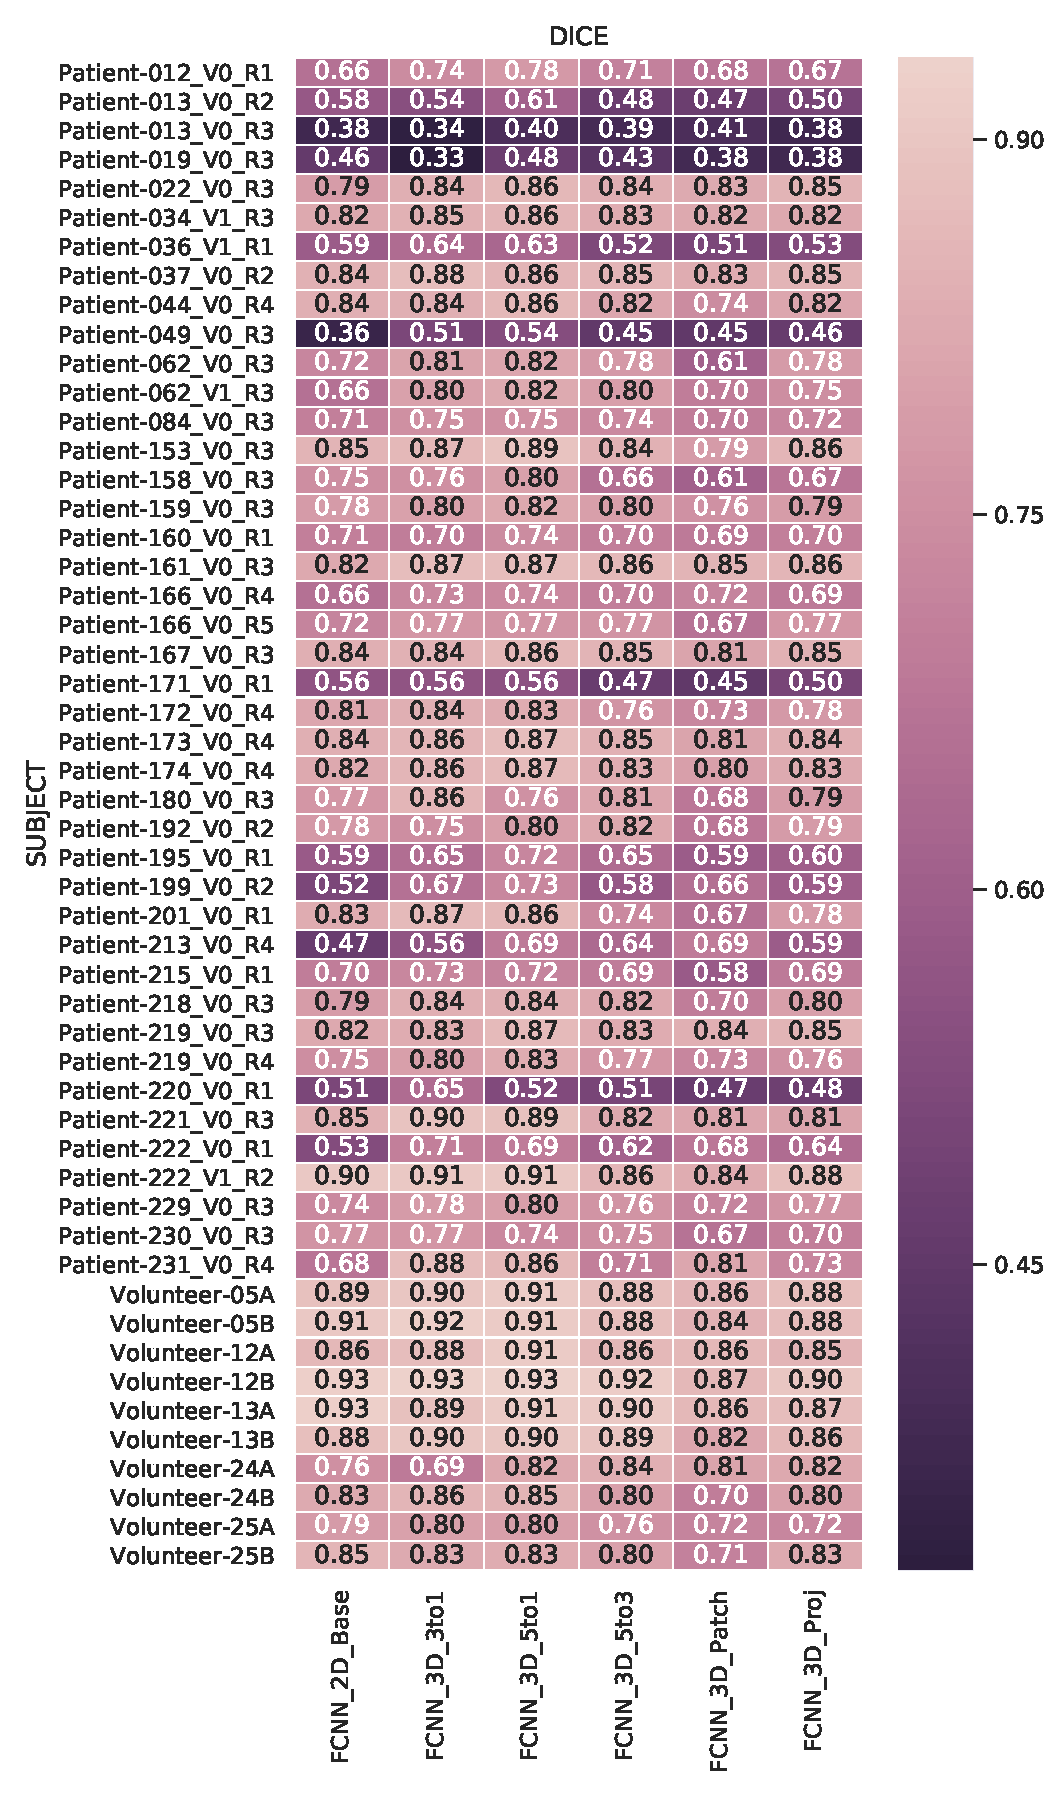
\includegraphics[width=\textwidth,height=\textheight,keepaspectratio]{heat_dice}
    \caption[Heatmap for the \acrlong{dice} for 3-D Context]{Heatmap for the achieved \acrlong{dice}s of the different neural network architectures.}
    \label{fig:results_heatmap_dice}
\end{figure}


\section{Experiment 3: Post-processing} \label{sec:exp_pp} % ====================================================
We applied the developed post-processing to the baseline and stack-based (5 to 1 slices) architecture. Post-processing was done on a desktop computer with a 6-core Intel i7 processor, and took approximately 3 minutes for keeping the $n$ largest volumes only (\textit{Volumes only}) for all 52 subjects. The number of volumes to keep was tuned for both architectures, resulting in $n = 3$ and $n = 2$ volumes for the baseline and stack-wise architecture, respectively. Joining the volumes and then keeping only the largest one (\textit{Joint volumes}) took one hour to process for all 52 subjects. Table~\ref{tab:results_pp_small} presents the obtained results with respect to the \acrlong{dice}, \acrlong{vs}, and \acrlong{hd95} (see Table~\ref{tab:results_pp} for all metrics). The overlap-based metrics were not influenced much by the post-processing but highly affected the \gls{hd95}. The boxplot in Figure~\ref{fig:pp_boxplots_hd95} shows the \acrlong{hd95} for the post-processing (see Figures~\ref{fig:pp_boxplots_vs} to \ref{fig:pp_boxplots_hd} for the other metrics). The influence of the post-processing is further shown in Figure~\ref{fig:pp_patient_219}.

\begin{table}[htbp]
   \centering
   \caption[Results for Post-processing]{Mean and \gls{sd} of the \acrlong{dice}, \acrlong{vs}, and \acrlong{hd95}. Post-processing was applied to the baseline and the stack architecture. \textit{Volumes only}: the $n$ largest volumes were kept ($n = 3$ and $n = 2$ for the Base and Stack\_5to1 architecture). \textit{Joint volumes}: connects the correctly segmented volumes first, and then keeping only the largest one.}
   \begin{tabular}{l*{7}{l}}
      \toprule
      Cohort	& Network	& Post-processing	& DICE				& VS				& HD95\\
      			&					&					&					&					& (mm)\\
      \midrule
      Patient   & Baseline 	& None & $0.705 \pm 0.137$ & $\mathbf{0.883 \pm 0.097}$ & $16.285 \pm 16.896$\\
                &                	& Volumes only  & $0.711 \pm 0.145$ & $0.867 \pm 0.125$ & $20.364 \pm 20.125$\\
                &                	& Joint volumes & $\mathbf{0.722 \pm 0.136}$ & $0.873 \pm 0.125$ & $\mathbf{11.812 \pm 12.785}$\\
      \cmidrule{2-6}
                & Stack\_5to1 	& None & $0.765 \pm 0.123$ & $0.898 \pm 0.110$ & $12.418 \pm 19.104$\\
                &                	& Volumes only  & $0.772 \pm 0.120$ & $0.899 \pm 0.119$ & $11.481 \pm 16.706$\\
                &                	& Joint volumes      & $\mathbf{0.779 \pm 0.123}$ & $\mathbf{0.905 \pm 0.117}$ & $\mathbf{6.688  \pm 10.332}$\\
      \midrule
      Volunteer & Baseline 	& None & $0.861 \pm 0.057$ & $0.921 \pm 0.056$ & $1.644  \pm 2.321 $\\
                &                	& Volumes only  & $0.862 \pm 0.057$ & $0.924 \pm 0.056$ & $2.311  \pm 4.508 $\\
                &                	& Joint volumes      & $\mathbf{0.868 \pm 0.050}$ & $\mathbf{0.929 \pm 0.056}$ & $\mathbf{1.230  \pm 1.255}$\\
      \cmidrule{2-6}
                & Stack\_5to1 	& None & $0.884 \pm 0.046$ & $0.927 \pm 0.051$ & $1.140  \pm 1.344 $\\
                &                	& Volumes only  & $0.883 \pm 0.046$ & $0.933 \pm 0.049$ & $1.357  \pm 1.454 $\\
                &                	& Joint volumes      & $\mathbf{0.894 \pm 0.042}$ & $\mathbf{0.942 \pm 0.050}$ & $\mathbf{0.655  \pm 0.355}$\\
      \bottomrule
   \end{tabular}
   \label{tab:results_pp_small}
\end{table}

\begin{figure}[htbp]
	\centering
	\subfloat[]
	{
		\label{fig:subfig:pp_boxplot_base_hd95}
		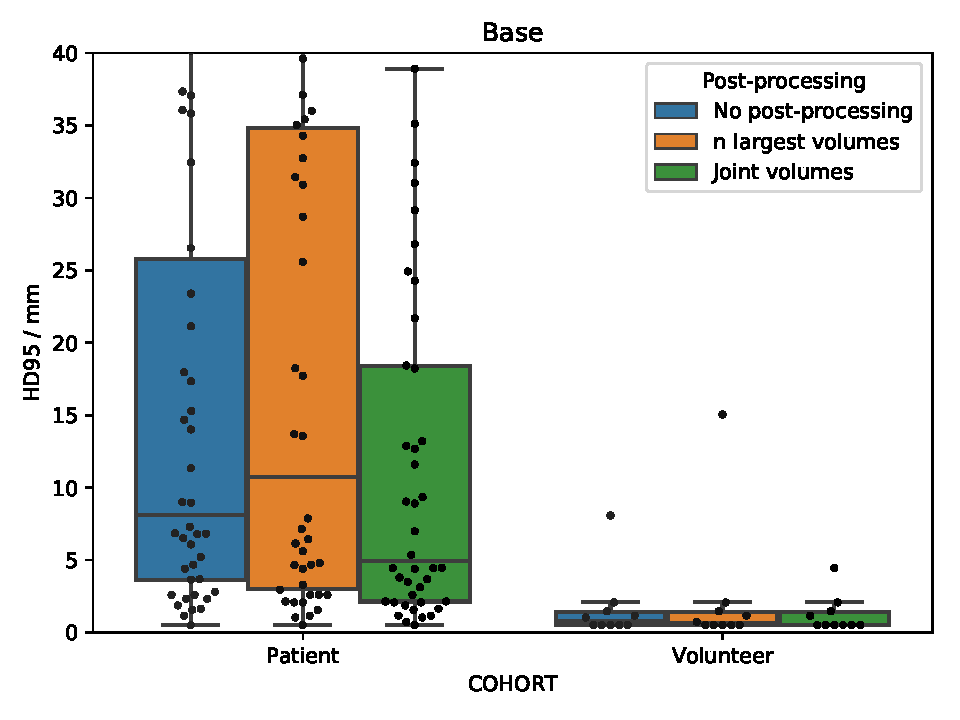
\includegraphics[width=0.7\textwidth]{pp_boxplot_base_HD95}
	}
	\hfill
	\subfloat[]
	{
		\label{fig:subfig:pp_boxplot_5to1_hd95}
		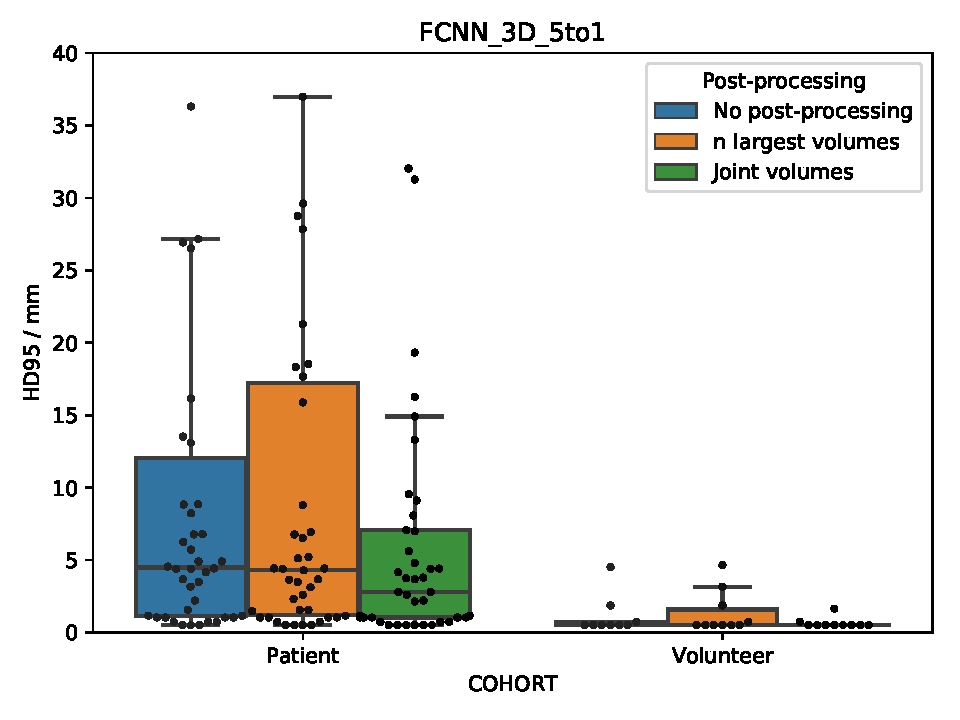
\includegraphics[width=0.7\textwidth]{pp_boxplot_5to1_HD95}
	}
	\caption[Boxplots of the \acrlong{hd95} for the post-processing]{Boxplots of the \acrlong{hd95} for the \textbf{a)} baseline and \textbf{b)} best performing stack-wise architecture with post-processing.  \textit{Volumes only}: the $n$ largest volumes were kept ($n = 3$ and $n = 2$ for the Base and Stack\_5to1 architecture). \textit{Joint volumes}: connects the correctly segmented volumes first, and then keeping only the largest one.}
	\label{fig:pp_boxplots_hd95}  
\end{figure}


\begin{figure}[htbp]
	\centering
	\subfloat[]
	{
		\label{fig:subfig:pp_base_219}
		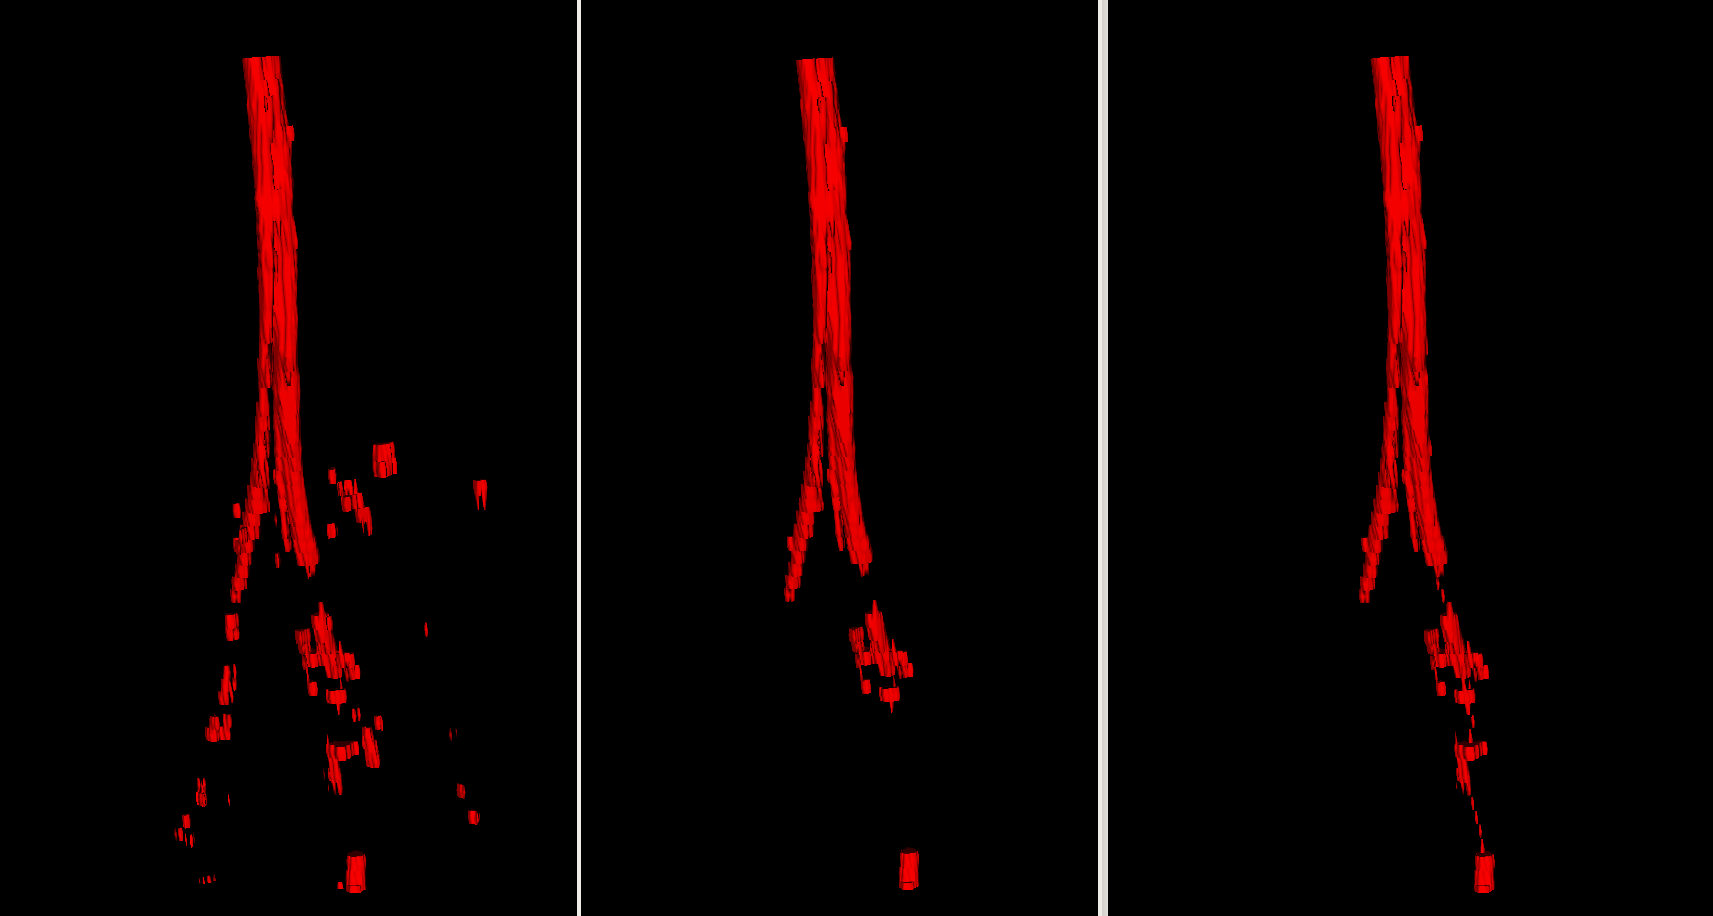
\includegraphics[width=\textwidth]{pp_base_219}
	}
	\hfill
	\subfloat[]
	{
		\label{fig:subfig:pp_5to1_219}
		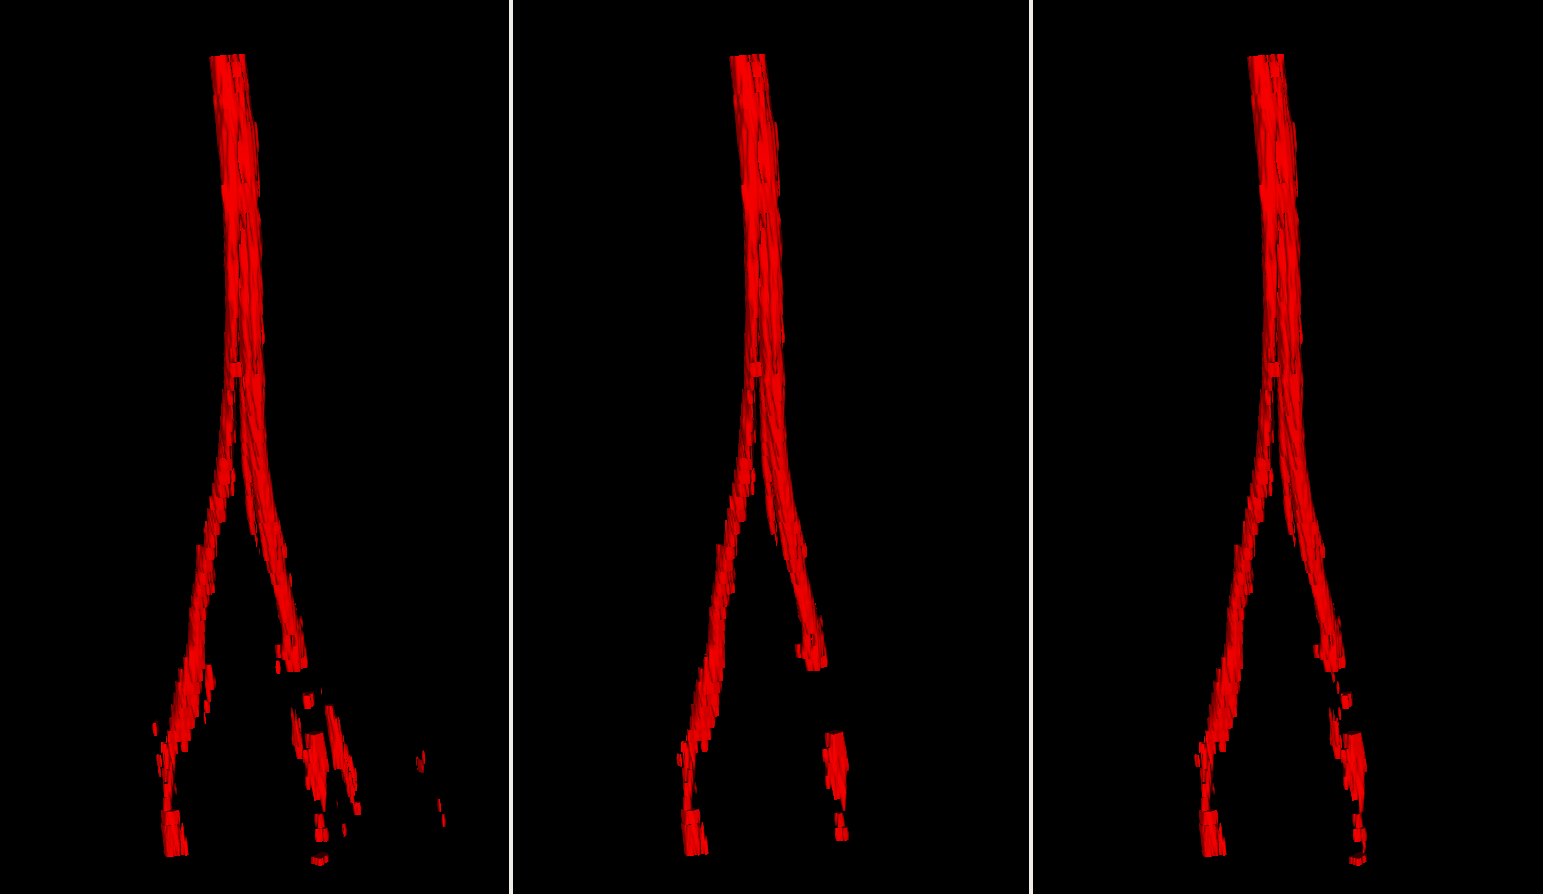
\includegraphics[width=\textwidth]{pp_5to1_219}
	}
	\caption[Segmentations Renderings]{Effect of the post-processing illustrated with \gls{3d} renderings of a segmented patient's sciatic nerve. \textbf{a)} Output segmentation of the baseline without post-processing (left), with $n$ largest volumes only (center), and with \textit{joint volumues} post-processing (right). \textbf{b)} Output segmentation of the best performing stack-wise architecture without post-processing (left), with $n$ largest volumes only (center), and with \textit{joint volumes} post-processing (right).}
	\label{fig:pp_patient_219}  
\end{figure}

\section{Comparison to Human Inter-Rater Performance} \label{sec:exp_evaluation} % ===============================================================
We compared the best performing architecture to the inter-rater agreement. The best performing architecture is the Stack-wise 5to1 with the \textit{joint volumes} post-processing (FCNN-GT; $n = 52$). The inter-rater agreement was obtained as described in Section~\ref{sec:eval_baseline} (R-R; $n = 156$).
Table~\ref{tab:res_fcnn_rater_small} summarizes the achieved \acrlong{dice}, \acrlong{vs}, and \acrlong{hd95}. Our proposed method achieves higher \gls{dice} values than the inter-rater performance. The $p$-values and the statistical significance of the comparison are gathered in the Table~\ref{tab:res_fcnn_rater_statistics}. Only for the volunteer \gls{dice} score, the difference is statistically significant. Hence, from a statistical point of view, our method is on par with the human inter-rater performance, or even surpassing it in the case of the \acrlong{dice} for the volunteer cohort.
Figure~\ref{fig:results_eval_boxplot_dice} shows the corresponding boxplot of the \acrlong{dice}. A detailed table (Table~\ref{tab:res_fcnn_rater}) and additional figures  are presented in the appendix.
In Figure~\ref{fig:res_inter_rater} the inter-rater agreement is shown as a heatmap for all the rater-to-rater and rater-to-ground-truth combinations.

\begin{table}[htbp]
   \centering
   \caption[Results for Comparison to Inter-Rater Performance]{Mean and \gls{sd} of the \acrlong{dice}, \acrlong{vs}, and \acrlong{hd95} achieved when comparing the best performing FCNN (Stack\_5to1 with full post-processing) to the inter-rater performance (R-R).}
   \begin{tabular}{l*{8}{l}}
      \toprule
      Cohort	& Comparison & DICE              & VS				& HD95\\
      			&			&					&					& (mm)\\
      \midrule
        Patient     & FCNN-GT & $0.779 \pm 0.123$ & $\mathbf{0.905 \pm 0.117}$ &                     $\mathbf{6.688  \pm 10.332}$ \\
                    & R-R     & $\mathbf{0.786 \pm 0.093}$ & $0.897 \pm 0.087$ &                     $11.245 \pm 19.008$ \\
        \midrule
        Volunteer   & FCNN-GT & $\mathbf{0.894 \pm 0.042}$ & $\mathbf{0.942 \pm 0.050}$ &                     $\mathbf{0.655  \pm 0.355} $ \\
                    & R-R     & $0.869 \pm 0.031$ & $0.937 \pm 0.043$ &                     $0.703  \pm 0.672 $ \\
      \bottomrule
   \end{tabular}
   \label{tab:res_fcnn_rater_small}
\end{table}


\begin{table}[htbp]
   \centering
   \caption[Statistics for Comparison to Inter-Rater Performance]{Statistical significance and $p$-values for the conducted unpaired Mann-Whitney U test (95 \% confidence interval) for the comparison to human inter-rater performance.}
   \begin{tabular}{l*{3}{l}}
      \toprule
        Cohort	    & Metric        & $p$       & Statistically significant\\
      			    &               &           &($p < 0.05$)          \\
      \midrule
        Patient     & \gls{dice}    & 0.60      & No\\
                    & \gls{vs}      & 0.60      & No\\
                    & \gls{avd}     & 0.31      & No\\
                    & \gls{hd95}    & 0.54      & No\\
                    & \gls{hd}      & 0.29      & No\\
        \midrule
        Volunteer   & \gls{dice}    & 0.02      & Yes\\
                    & \gls{vs}      & 0.65      & No\\
                    & \gls{avd}     & 0.70      & No\\
                    & \gls{hd95}    & 0.48      & No\\
                    & \gls{hd}      & 0.18      & No\\
      \bottomrule
   \end{tabular}
   \label{tab:res_fcnn_rater_statistics}
\end{table}

\begin{figure}[htbp]
	\centering
	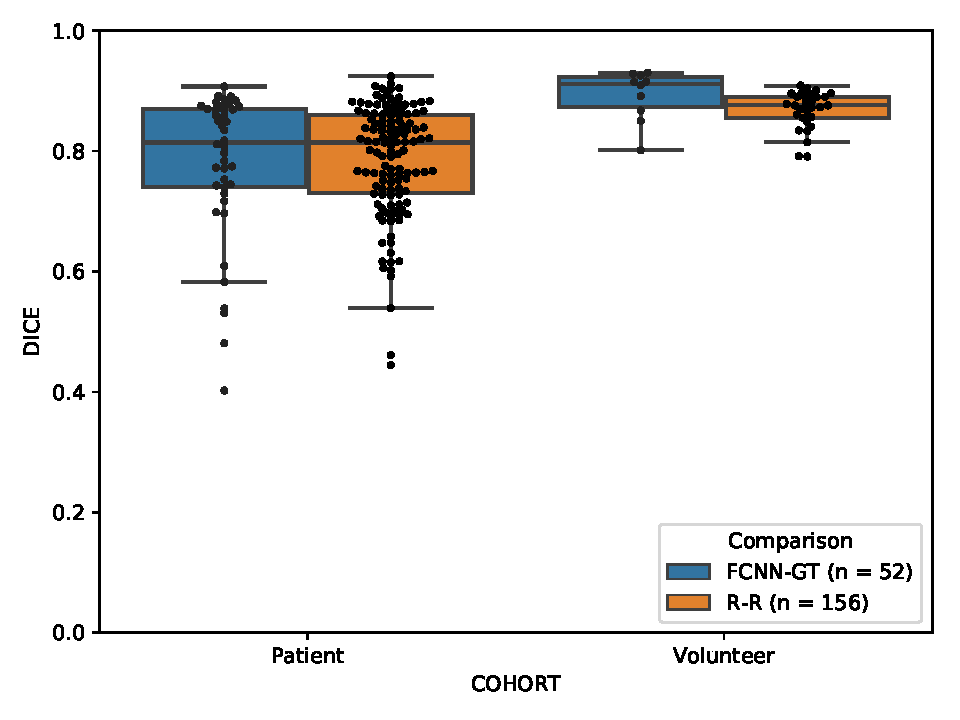
\includegraphics[width=\textwidth]{boxplot_eval_DICE}
    \caption[Boxplot of the \acrlong{dice} compared to the inter-rater performance]{Boxplot of \acrlong{dice} with the best performing architecture (FCNN-GT) and the inter-rater (R-R) performance.}
    \label{fig:results_eval_boxplot_dice}
\end{figure}

\begin{figure}[htbp]	
	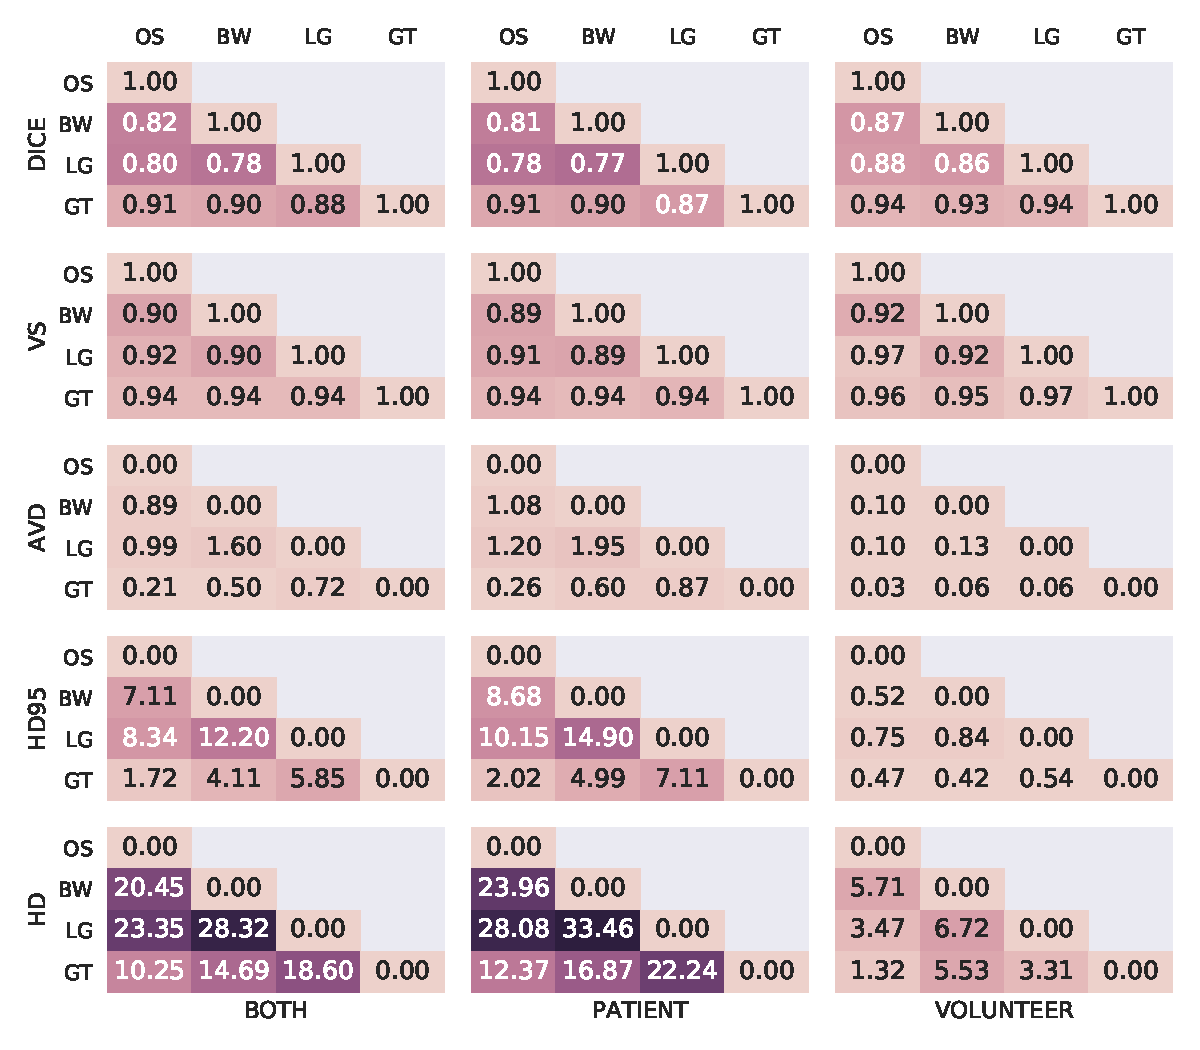
\includegraphics[width=\textwidth]{inter_rater}
    \caption[Heatmap for Inter-Rater Agreement]{Inter-rater agreement for the \acrlong{dice}, \acrlong{vs}, \acrlong{avd}, \acrlong{hd95} and \acrlong{hd} per cohort. Values close to 1.00 for \gls{dice} and \gls{vs} correspond to a high level of agreement between the raters. Conversely, low values for \gls{avd}, \gls{hd95} and \gls{hd} imply higher agreement.}
    \label{fig:res_inter_rater}
\end{figure}

\section{Time Requirements} \label{sec:res_times}
Table~\ref{tab:results_durations} contains all the different times required for the individual steps involved in the peripheral nerve segmentation. Note that the fully-automatic segmentation of one \gls{mrn} case, including registration (1 $\pm$ 0.5 minute), segmentation by the neural network (3 seconds) and \textit{joint volumes} post-processing (1 minute), takes a total of 2 $\pm$ 0.5 minutes.

\begin{table}[htbp]
   \centering
   \caption[Time Requirements]{Time requirements for the different steps involved in the peripheral nerve segmentation. All durations are given as the time required to process a single \gls{mrn} case.}
   \begin{tabular}{l*{3}{l}}
      \toprule
      Step                  & Variant               & Duration\\
      \midrule
      Training              & Base                  & 2 h   \\
                            & Stack (all)           & 15 h  \\
                            & Patch                 & 22 h  \\
      \midrule
      Registration          &                       & $1 \pm 0.5$ min \\
      \midrule
      Segmentation          &                       & 3 s \\
      Post-processing       & $n$ largest volumes   & 4 s \\
                            & Joint volumes         & 1 min \\
      \midrule
      Fully-automatic segmentation & & 2 $\pm$ 0.5 min\\
      (After training, full post-processing)\\
      \midrule
      Manual ground truth segmentation & & $19 \pm 8$ min\\
      (done by expert) \\
      \bottomrule
   \end{tabular}
   \label{tab:results_durations}
\end{table}

\endinput
\chapter{Discussion and Conclusions} \label{chap:discussion_and_conclusions}
This chapter provides a discussion on the obtained results in Section~\ref{disc:discussion}. After the discussion, a conclusion on the outcome of this thesis is given in Section~\ref{disc:conclusions}.

\section{Discussion} \label{disc:discussion}
\subsection{Feasibility of Deep Learning for Peripheral Nerve Segmentation}
We successfully trained the baseline architecture on the \gls{mrn} images, achieving better results than reported in Balsiger et al. \cite{Balsiger2016DevelopmentApproaches} with the \gls{rf}-based approach. The results are in accordance with their recent deep learning-based approach~\cite{Balsiger2018SegmentationApproach}. Therefore, a deep learning-based approach for the peripheral nerve segmentation is feasible.
Comparing the results between the cohorts shows that our baseline performed better on the volunteer cohort. We suspect that the main reason for this discrepancy is the higher variability in the clinically acquired patient images. While the \gls{mrn} images for the volunteers were all taken from the same anatomical location, the images of the patients originate from variable locations between the distal thigh up to the head of the femur. An investigation of the segmentations shows a high prevalence of false positive outliers and occasionally false negatives, visible as slice-wise gaps along the nerve course. Outliers were often segmented where blood vessels are present in the \gls{mrn} images, whereas the slice-wise gaps seem to be an inherent artifact of the \gls{2d} approach.\\
The patient \gls{mrn} images tend to have more movement artifacts compared to the volunteer \gls{mrn} images. These artefacts make the image registration during the pre-processing more complex. To investigate a potential influence of the registration, we trained the baseline architecture on each of the \gls{mrn} images separately. Using only the T2 images, we were able to perform almost as good as when trained with both images (IR and T2). However, using only the IR images resulted in a worse \acrlong{dice} and a higher \acrlong{hd95}. It seems that the neural network was not able to learn the same quality of features and therefore to extract the same amount of information out of the IR images. We assume that a reason for the worse results might be that the unprocessed IR images have a lower in-plane resolution and are interpolated during the pre-processing. Another reason may be that it is inherently harder, even for human experts, to correctly segment nerves only using the IR image. Hence, the task given to the neural network was harder in the first place. Furthermore, we suspect that the registration might be another issue: A subject-level investigation showed that there are cases where the registration is of low quality, hence there is misalignment between the IR and T2 images. Consequently, the IR images are also misaligned to the ground truths because the physicians used the T2 images for their manual ground truth segmentation. Such a misalignment is especially relevant for small structures as peripheral nerves. The misalignment might make it more complicated for the neural network to learn useful features from the IR images than from the T2 images. Interestingly, the IR image is useful for the segmentation in regards to the \gls{hd95} metric. The combination of the T2 and IR image for training resulted in the reduction of the \acrlong{hd95} from 17.522$\pm$17.218 mm and 5.909$\pm$12.433 mm (trained on T2 image only) down to 16.526$\pm$17.025 mm and 1.644$\pm$2.321 mm for the patient and volunteer cohort, respectively. This reduction of the \gls{hd95} means that the IR image helps to reduce false positive outliers, especially in case of the volunteer cohort. An investigation of the subjects reveals that often blood vessels get segmented as nerves in the case of T2 only, probably due to their similar appearance to peripheral nerves on this \gls{mrn} sequence (cf. Figure~\ref{fig:subfig:T2}). The IR image, therefore, seems to help the network distinguish the nerve from blood vessels and other neighboring tissue. These findings align with the thinking pattern of physicians and the choice of the MRN sequences at the Inselspital: the T2 image is used for the coarse localization of the nerves and the IR image for the finer analysis due to the slightly hyper-intense appearance of nerves compared to the mostly surrounding tissue and blood vessels. These results motivated us to continue with the IR and T2 combination as input in our further experiments.

\subsection{Tailored 3-D Information for Peripheral Nerve Segmentation}
We successfully trained and evaluated the proposed neural networks with different degrees of access to \gls{3d} information. The stack-based method achieved almost constantly better results than the \gls{2d} baseline. The projection-based and patch-based methods resulted in worse performance. Our best performing method, stack-based 5-to-1, is on par or outperforms the method proposed by Balsiger et al.~\cite{Balsiger2018SegmentationApproach} with respect to the \acrlong{dice} and \acrlong{hd95}, achieving only slightly worse results concerning the \acrlong{vs}. Our mean and \gls{sd} of the \gls{hd95} of 12.4 $\pm$ 19.1 mm for the patient cohort are slightly larger than the \gls{hd95} of 12.4 $\pm$ 12.1 mm they reported. Our mean and \gls{sd} of the \gls{hd95} of 1.5 $\pm$ 1.8 mm for the volunteer cohort, on the other hand, are significantly lower than theirs of 13.9 $\pm$ 26.6 mm.\\
The gain in performance with \gls{3d} information is, in general, higher for the patient cohort. This is mainly due to the reason that the \gls{2d} baseline architecture is already achieving good segmentation performance for the volunteer cohort and that there is not much space to improve. We still observe some false positive outliers in the segmentation results of the \gls{3d} architectures, however in reduced numbers. Furthermore, the false negative gaps are less frequent. In general, the stack-wise architectures can detect and segment the sciatic nerve in some cases where the baseline architecture failed.\\
We consistently achieved the best results concerning \acrlong{dice} and \acrlong{vs}, with the stack-based 5-to-1 architecture for both cohorts. Regarding the distance-metrics, the stack-based 3-to-1 and stack-based 5-to-3 performed the best for patient and volunteer cohort, respectively. However, seen over all metrics, the stack-based 5-to-1 neural network is performing the most robust. The architecture seems adequate and well suited for the task at hand for the intrinsic parameters (high in-plane resolution, large z-spacing) of our \gls{mrn} images.\\
Both stack-based 5-to-3 architectures (Stack\_5to3 and Stack\_Proj) did perform worse compared to the other \gls{3d} architectures, especially on the patient cohort. Therefore, for the segmentation of our \gls{mrn} images, predicting multiple slices at once with our configuration does not bring any benefit. Performance could potentially be increased, by reducing the axial stride from three down to one, resulting in each slice being predicted three times. The predictions could then be averaged for the segmentation. We used zero-filling to predict the most proximal and the most distal slice. However, it would be worth investigating whether a more sophisticated way, i.e., copying of actual image data instead of zero-filling, influences the segmentation quality of these slices.
Training the stack-based 5-to-3 architecture with the projection loss resulted in almost the same performances as the same architecture with the regular loss function, except for the \acrlong{avd}, which was nearly twice as large, in case of the volunteer cohort. An investigation of the volunteer \gls{mrn} cases revealed that there are more false positive outliers present in the segmentations of the projection-based loss. However, we think this loss function could be potentially useful for the incorporation of, e.g., anatomical shape priors during the training phase. Therefore, training of neural networks with this loss needs further investigation.\\
The patch-based network performed the worst with regards to all metrics, even when compared to the baseline architecture. Despite having access to the \gls{3d} information of 12 consecutive slices, the reduction of the accessible in-plane information seems to restrict the neural network drastically in its segmentation capabilities. This emphasizes the importance of the in-plane context. However, we suspect a problem of our patch-based approach might be the fact that we use \textit{same}-padding and predict the same dimensions as the input. We think that \textit{valid}-padding and consequently predicting a smaller region might produce better results due to the network's receptive field.\\
Analyzing the heatmap of the achieved \gls{dice}s in Figure~\ref{fig:results_heatmap_dice}, three things become evident: First, all architectures perform better on the volunteer cohort. We already observed this in the previous experiment, and \gls{3d} context does not change this result. Second, the subjects where low performances were achieved, predominantly patients, are generally the same for all architectures. Hence, there are subjects which are inherently hard for all architectures to segment with high accuracy. Third, most of these subjects are patient subjects which have been examined and enrolled in an earlier stage in the registry. In some of these subjects, patient movement artifacts are noticeable. This suggests that the \gls{mrn} imaging protocol in the earlier stages was not optimal, and then subsequently got adjusted. Assessment of these subjects in the form of an outlier-analysis could be advisable.\\
In summary, we found that introducing \gls{3d} information can increase the performances to a certain extent. We also found that architectural changes as the number of features and number of input slices play a secondary role. More important is the general architecture, which has to adequate for the problem and the given data: in our case, a good mix between \gls{2d} and \gls{3d} convolutions, with a more dominant \gls{2d} part was the solution. This, given the intrinsic properties of our \gls{mrn} images, intuitively makes sense and is also in accordance with the results of Baumgartner et al.~\cite{Baumgartner2017AnSegmentation}. We, therefore, conclude that \gls{3d} context allows for better segmentation performance, given the right circumstances.

\subsection{Post-processing for Peripheral Nerve Segmentation}
We successfully applied our post-processing to the outputs of the baseline and stack-based 5-to-1 architectures. For both cohorts, joining the volumes and subsequently removing of all but the largest volumes (\textit{joint volumes} post-processing) yields the best segmentation performances with regard to all metrics. The single exception is the patient \acrlong{vs} of the baseline architecture, where no post-processing results in a higher \gls{vs}.\\
The post-processing was mainly motivated by the false positive segmentations. Therefore, the impact of post-processing on the distance metrics \gls{avd}, \gls{hd95} and \gls{hd} is far more dominant than on the overlap-based metrics, i.e., \gls{dice} and \gls{vs}. Inspection of the segmentation reveals that most of the false positive outliers can be removed by our post-processing, resulting in the significant better results for the distance metrics.
Concerning the \acrlong{hd95}, our post-processing benefits the stack-based 5-to-1 architecture even more than the baseline: the \gls{hd95} is reduced by approximately 45 \% for the stack-based approach, and reduced by about 25 \% for the baseline.\\
A limitation of our post-processing method is the calculation of the cheapest path for the volume connection: we only consider one path (the cheapest of all paths). This is applicable and fine for the cases that do not include the branching of the sciatic nerve. For the cases that include the branching, a better way would be to calculate two paths: both would start proximally in the sciatic nerve, and then after the branching follow the tibial and fibular nerve, respectively.
Furthermore, calculating the cheapest paths corresponds to find the centerline of the nerves. Centerlines have been found be useful for e.g. in blood vessels segmentation~\cite{Lesage2009ASchemes} and could be used for further refinement. We could extend the post-processing to result in an additional map that contains the pixels belonging to the cheapest paths and therefore designating the centerlines of the nerves.\\
Alternatively, perhaps more sophisticated methods of post-processing, similar to~\cite{Rempfler2015ReconstructingProgramming} and~\cite{Selvan2018ExtractionNetworks} could be applied to increase and solidify the segmentation performance even further. 

\subsection{Comparison to Human Inter-Rater Performance}
We took our best-performing architecture (Stack\_5to1) and compared the post-processed (\textit{joint volumes}) segmentation results to the human inter-rater performance. Our inter-rater study reveals that we achieve, or in the case of the \acrlong{dice} for the volunteer cohort even surpass, human-level segmentation performances from a quantitative and statistical point of view. Nevertheless, in some cases, it was still quite easy to distinguish between a segmentation done by an expert and a segmentation resulting from our method: sometimes our method segmented regions which, given the anatomical shape of the nerve, obviously could not belong to the nerve.\\
Looking at inter-rater agreement values for the metrics in Figure~\ref{fig:res_inter_rater} reveals that sciatic nerve segmentation is and remains a challenging task even for experts, and requires years of experience (agreement of OS to GT compared to the less experienced LG and BW). This puts the results of our method more into perspective and shows how, in fact, impressive the achieved segmentation performances are.\\
Comparing the time required for our fully-automatic method with the time required for an expert to manually segment a \gls{mrn} image, we see that our method results in a significant time gain for sciatic nerve segmentation.\\


\section{Conclusions} \label{disc:conclusions}
In our first experiment, we showed the feasibility of a deep learning-based approach for the segmentation of the sciatic nerve. Moreover, we showed training only on the T2 image was almost able to achieve the same results as when both images are used. Still, the neural network is able to extract useful information from the IR image. Therefore, training on both \gls{mrn} images is advisable.\\
We demonstrated in our second experiment that \gls{3d} context is indeed allowing for better segmentation performances. The amount of useful \gls{3d} context, however, heavily depends on the task at hand and the nature of the data. For our \gls{mrn} images, which have a high in-plane resolution, a large slice spacing, and a low axial resolution, a stack-wise architecture that allows for a tailored amount of \gls{3d} context achieved the best results.\\
With the use of post-processing, we showed that segmentations of the neural networks could be enhanced. While the impact of post-processing on the overlap-based metrics was rather small, the distance-metrics profited a lot.\\
The segmentation of the sciatic nerve, or peripheral nerves in general, from \gls{mrn} images remains a challenging but possibly important task. The segmentation could help clinicians in the diagnosis and monitoring of peripheral neuropathies, and could be used to calculate potentially useful image-derived biomarkers such as the \gls{fnr} and the \gls{csa}. A fast, robust and fully-automatic segmentation method is therefore desirable and beneficial. Finally, we showed in comparison with the inter-rater performance, that our method achieves or surpasses human-level segmentation performance concerning all metrics. Furthermore, our method requires significantly less time for the segmentation than manual segmentation.

\endinput
\chapter{Outlook} \label{chap:outlook}
The developed method segments the sciatic nerve with human-level performance regarding quantitative evaluation metrics. As we aim to leverage the diagnosis and the assessment of all peripheral nerves, obviously future work should go in the direction of a method that can segment all peripheral nerves. Although not used in this work, we have further \gls{mrn} images available from different anatomical regions (upper \& lower arm, lower leg) for the volunteer cohort and also the patients in the registry. A method could be developed incorporating these \gls{mrn} images. However, given that the sciatic nerve is the largest nerve in the human body, segmenting smaller peripheral nerves might be difficult. Almost certainly a large number of \gls{mrn} images with higher resolution would be required to achieve an acceptable level of segmentation performance. Once peripheral nerves can robustly be segmented, potentially new biomarkers, such as texture analysis-based biomarkers~\cite{FelisazTextureNeuropathy}, could be extracted from the \gls{mrn} images and used for assessment and diagnosis of neuropathies. However, the development of biomarkers might require matched cohorts to be clinically meaningful. Furthermore, an expert assessment in the form of an outlier-analysis could be an advisable next step to do on our \gls{mrn} images. As we showed in the first experiment, the trained neural networks mainly relying on the \gls{t2} images. However, the \gls{ir} images reduced false positive outliers and helped the network to distinguish between nerve and blood vessels. Therefore, it is crucial to further refine and optimize the \gls{mrn} sequences for even better imaging of the nerves. Both, clinicians and methods like the one we proposed would be the direct benefactors.\\
Regarding technical developments, a point could be to reduce the axial spacing during the \gls{mrn} acquisition (e.g., \gls{3d} \gls{mrn} sequences) and reinvestigate the potential segmentation performance increase of \gls{3d} context.
Furthermore, the impact of the projection-based loss could be examined in more detail because it almost achieved achieved the same results as the cross-entropy loss. Perhaps more axial slices could be used to calculate the projections. Or maybe, a stack-wise 5-to-1 architecture could be expanded by two additional loss terms based on the sagittal and coronal projections. The projection-loss could be a way to incorporate a potential anatomical tubular-like shape prior into the learning phase of a neural network. Furthermore, we think that a combination of a neural network in conjunction with post-processing is the future method of peripheral nerve segmentation. Post-processing, however, could be more sophisticated than ours. Our post-processing method could be improved by taking multiple paths through the graph, in order to account for the branching of the nerve. One could also change to a more sophisticated method based on a probabilistic model with anatomical constraints, similarly to~\cite{Rempfler2015ReconstructingProgramming}.
\endinput

% Uncomment this if you'd like to suppress the numbering of the
% appendices.
%\backmatter

%%%%%%%%%%%%%%%%%%%%%%%%%%%%%%%%%%%%%%%%%%%%%%%%%%%%%%%%%%%%%%%%%%%%%
% Bibliography
%%%%%%%%%%%%%%%%%%%%%%%%%%%%%%%%%%%%%%%%%%%%%%%%%%%%%%%%%%%%%%%%%%%%%
% Force every reference to show up (demo)
\bibliography{mend}

%%%%%%%%%%%%%%%%%%%%%%%%%%%%%%%%%%%%%%%%%%%%%%%%%%%%%%%%%%%%%%%%%%%%%
% Appendices
%%%%%%%%%%%%%%%%%%%%%%%%%%%%%%%%%%%%%%%%%%%%%%%%%%%%%%%%%%%%%%%%%%%%%
\part*{Appendices}
\begin{appendix}
	\chapter{Results} \label{app:results}
\section{Experiment 1: Feasibility} % =============================================================================

\section{Experiment 2: 3D Context} % ==============================================================================

\begin{sidewaystable}[htbp]
   \centering
   \caption[Segmentation Evaluation Metrics for the different Architectures]{}
   \begin{tabular}{l*{6}{l}}
      \toprule
      Cohort	& Neural Network	& DICE				& VS				& AVD				& HD95				& HD				\\
      			&					&					&					& (mm)				& (mm)				& (mm)				\\
      \midrule
      Patient   & FCNN\_2D\_Base  & $0.704 \pm 0.139$ & $0.882 \pm 0.098$ & $2.880 \pm 2.671$ & $16.526 \pm 17.025$ & $63.696 \pm 20.903$ \\
                & FCNN\_3D\_3to1  & $0.749 \pm 0.139$ & $0.896 \pm 0.123$ & $\mathbf{1.979 \pm 2.190}$ & $\mathbf{10.807 \pm 13.393}$ & $\mathbf{56.262 \pm 23.958}$ \\
                & FCNN\_3D\_5to1  & $\mathbf{0.765 \pm 0.123}$ & $\mathbf{0.898 \pm 0.110}$ & $2.001 \pm 2.401$ & $12.418 \pm 19.104$ & $56.304 \pm 28.746$ \\
                & FCNN\_3D\_5to3  & $0.717 \pm 0.135$ & $0.883 \pm 0.105$ & $2.995 \pm 3.148$ & $19.312 \pm 22.545$ & $65.740 \pm 22.811$ \\
                & FCNN\_3D\_Proj  & $0.712 \pm 0.136$ & $0.889 \pm 0.094$ & $3.119 \pm 3.038$ & $19.878 \pm 21.613$ & $60.762 \pm 22.985$ \\
                & FCNN\_3D\_Patch & $0.682 \pm 0.128$ & $0.876 \pm 0.101$ & $3.581 \pm 2.724$ & $24.241 \pm 20.896$ & $70.737 \pm 26.853$ \\                
      \midrule
      Volunteer & FCNN\_2D\_Base  & $0.861 \pm 0.057$ & $0.921 \pm 0.056$ & $0.643 \pm 0.866$ & $1.644  \pm 2.321 $ & $\mathbf{35.380 \pm 32.720}$ \\
                & FCNN\_3D\_3to1  & $0.860 \pm 0.073$ & $0.925 \pm 0.043$ & $0.734 \pm 0.859$ & $2.260  \pm 2.336 $ & $39.327 \pm 29.429$ \\
                & FCNN\_3D\_5to1  & $\mathbf{0.878 \pm 0.048}$ & $\mathbf{0.928 \pm 0.048}$ & $ 0.509 \pm 0.393	$ & $1.537  \pm 1.784 $ & $46.515 \pm 30.853$ \\
                & FCNN\_3D\_5to3  & $0.855 \pm 0.052$ & $0.928 \pm 0.062$ & $\mathbf{0.473 \pm 0.435}$ & $\mathbf{1.350  \pm 1.365} $ & $39.033 \pm 30.589$ \\                
                & FCNN\_3D\_Proj  & $0.842 \pm 0.051$ & $0.917 \pm 0.067$ & $0.861 \pm 0.813$ & $1.642  \pm 1.549 $ & $40.584 \pm 30.139$ \\
                & FCNN\_3D\_Patch & $0.806 \pm 0.068$ & $0.888 \pm 0.085$ & $1.166 \pm 1.164$ & $7.992  \pm 13.474$ & $39.796 \pm 27.201$ \\
      \bottomrule
   \end{tabular}
   \label{tab:results_3d_context}
\end{sidewaystable}

\begin{figure}[htbp]
	\centering
	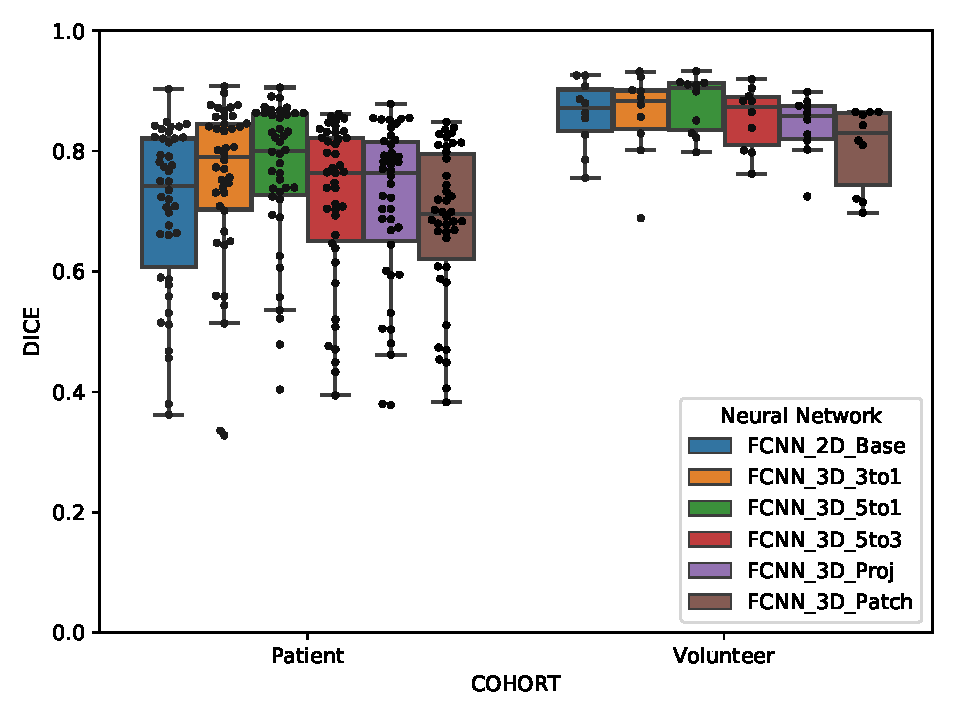
\includegraphics[width=0.8\textwidth]{boxplot_DICE}
    \caption[Boxplot for the \acrlong{dice}.]{Boxplot for the \acrlong{dice}.}
    \label{fig:results_boxplot_dice}
\end{figure}
\begin{figure}[htbp]
	\centering
	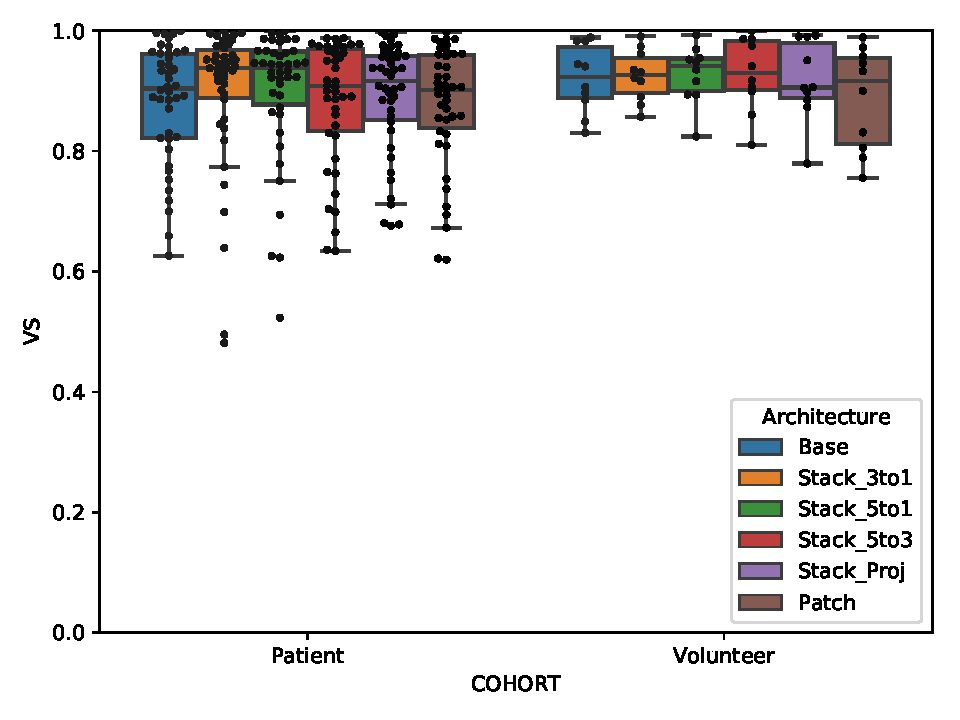
\includegraphics[width=0.8\textwidth]{boxplot_VS}
    \caption[Boxplot for the \acrlong{vs}.]{Boxplot for the \acrlong{vs}.}
    \label{fig:results_boxplot_vs}
\end{figure}
\begin{figure}[htbp]
	\centering
	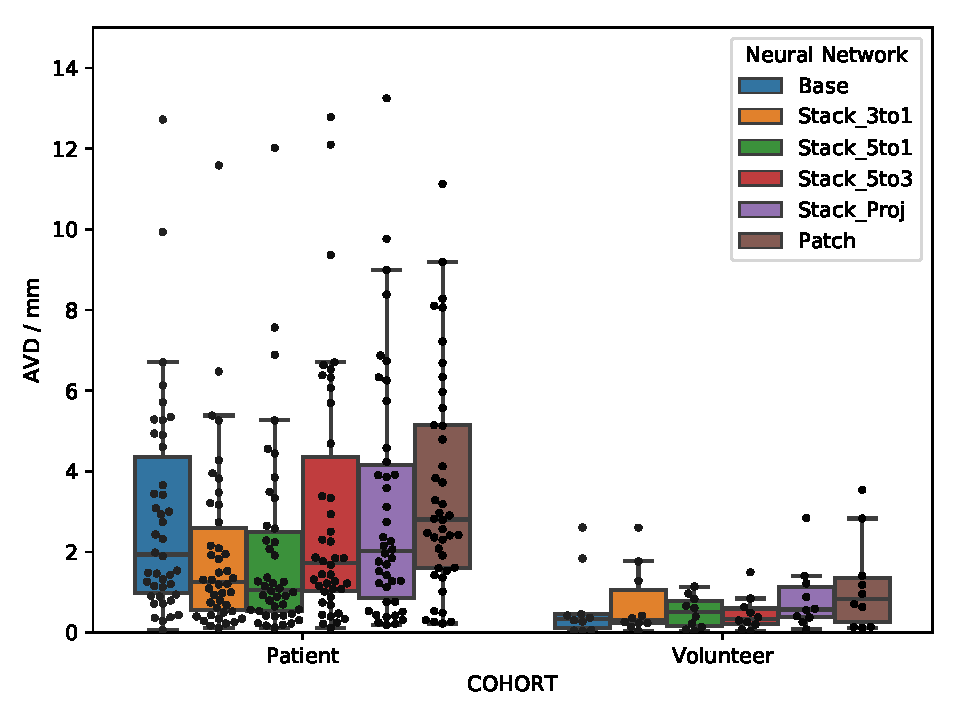
\includegraphics[width=0.8\textwidth]{boxplot_AVD}
    \caption[Boxplot for the \acrlong{avd}.]{Boxplot for the \acrlong{avd}.}
    \label{fig:results_boxplot_avd}
\end{figure}
\begin{figure}[htbp]	
	\centering
	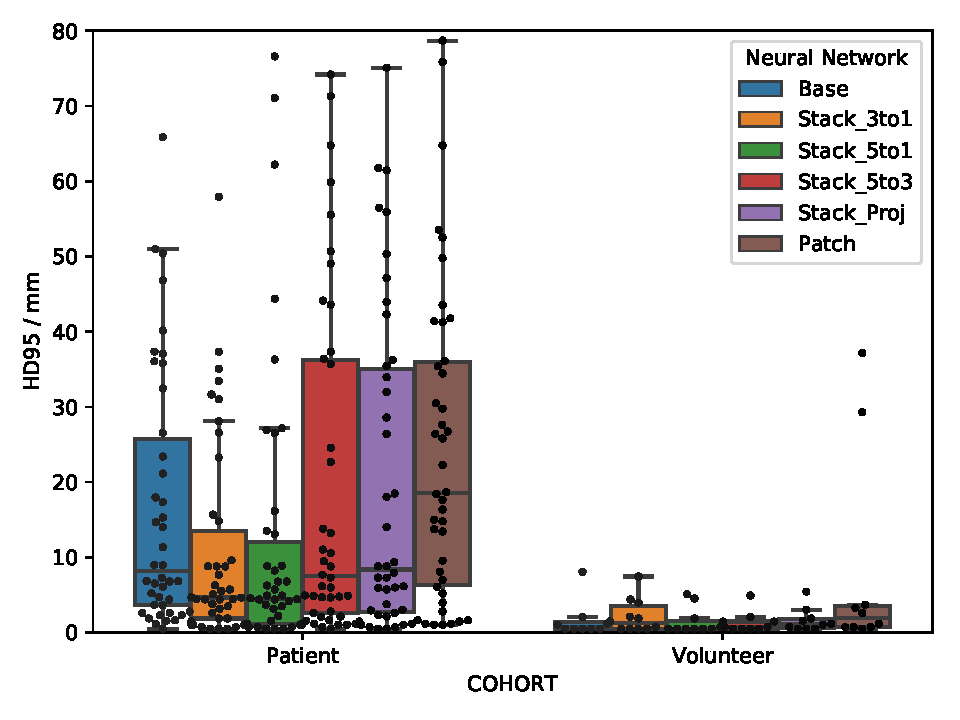
\includegraphics[width=0.8\textwidth]{boxplot_HD95}
    \caption[Boxplot for the 95\textsuperscript{th} percentile \acrlong{hd}.]{Boxplot for the 95\textsuperscript{th} percentile \acrlong{hd}.}
    \label{fig:results_boxplot_hd95}
\end{figure}
\begin{figure}[htbp]	
	\centering
	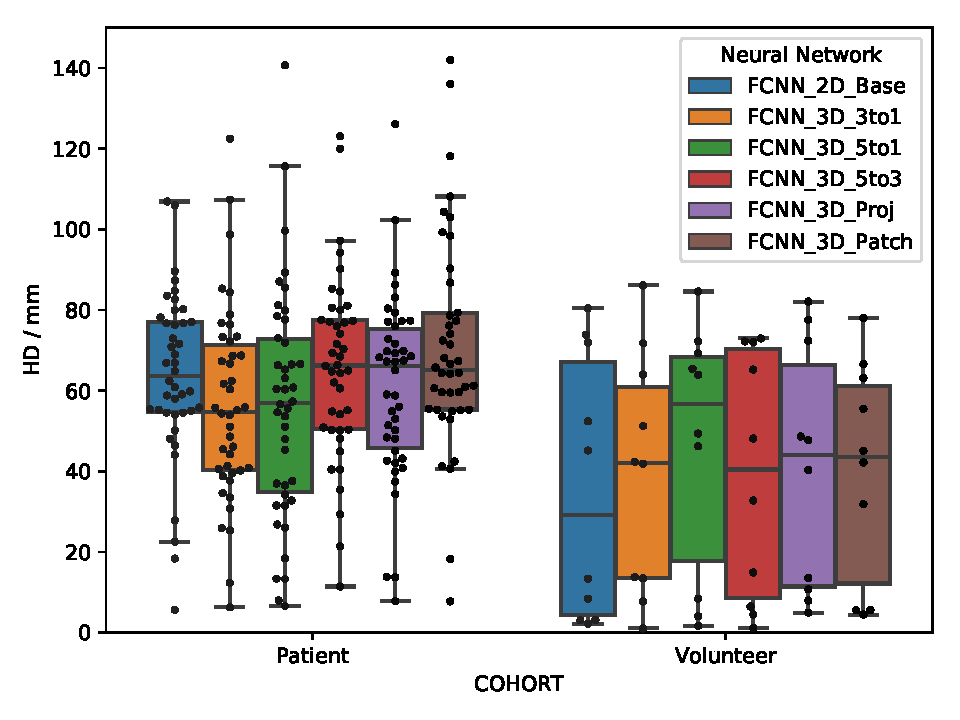
\includegraphics[width=0.8\textwidth]{boxplot_HD}
    \caption[Boxplot for the \acrlong{hd}.]{Boxplot for the \acrlong{hd}.}
    \label{fig:results_boxplot_hd}
\end{figure}

\begin{figure}[htbp]	
	\centering
	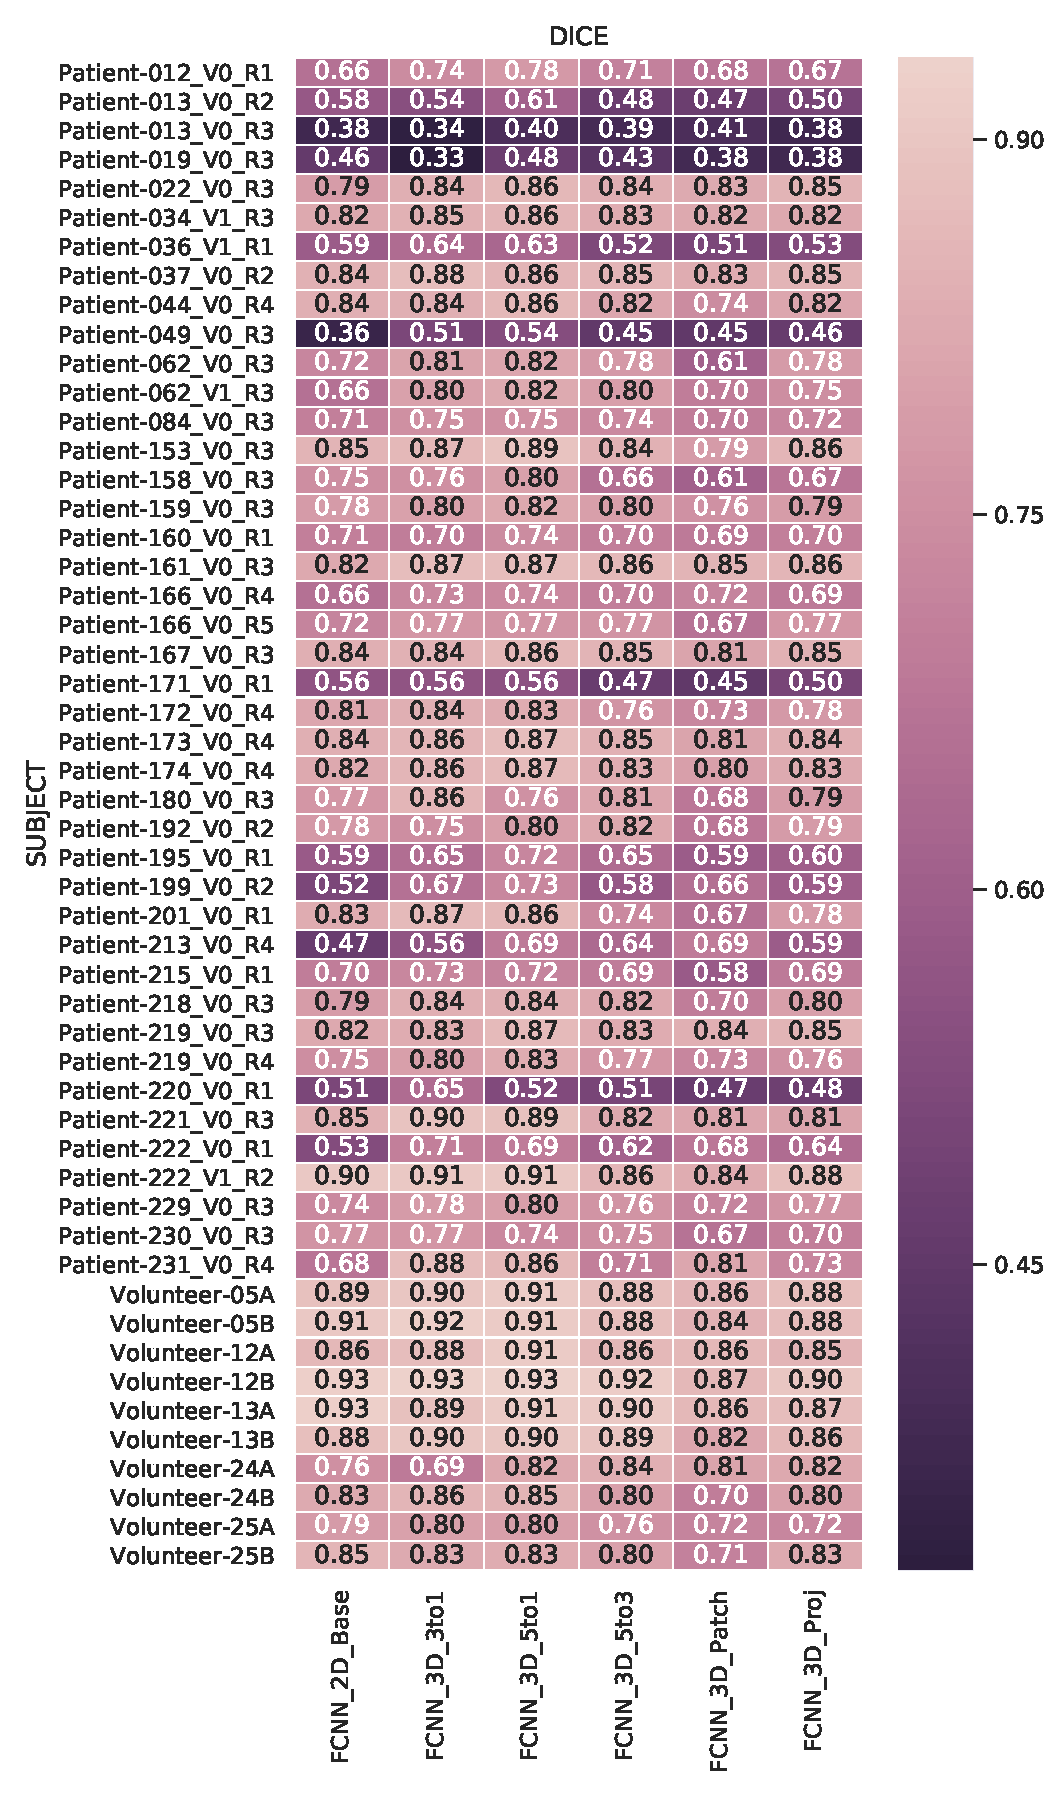
\includegraphics[width=\textwidth]{heat_dice}
    \caption[Heatmap for the \acrlong{dice}.]{Heatmap for the \acrlong{dice}.}
    \label{fig:results_heat_dice}
\end{figure}

\section{Experiment 3: Post-processing} % ===========================================================================

\begin{sidewaystable}[htbp]
   \centering
   \caption[Segmentation Evaluation Metrics for the different Architectures]{}
   \begin{tabular}{l*{7}{l}}
      \toprule
      Cohort	& Network	& Post-processing	& DICE				& VS				& AVD				& HD95				& HD				\\
      			&					&					&					&					& (mm)				& (mm)				& (mm)				\\
      \midrule
      Patient   & 2D\_Base 	& None & $0.705 \pm 0.137$ & $\mathbf{0.883 \pm 0.097}$ & $2.835 \pm 2.655$ & $16.285 \pm 16.896$ & $62.630 \pm 21.803$ \\
                &                	& Volumes only  & $0.711 \pm 0.145$ & $0.867 \pm 0.125$ & $3.431 \pm 4.236$ & $20.364 \pm 20.125$ & $50.726 \pm 21.318$ \\
                &                	& Joint volumes & $\mathbf{0.722 \pm 0.136}$ & $0.873 \pm 0.125$ & $\mathbf{1.705 \pm 1.768}$ & $\mathbf{11.812 \pm 12.785}$& $\mathbf{32.159 \pm 20.178}$ \\
      \midrule
      Patient   & 3D\_5to1 	& None & $0.765 \pm 0.123$ & $0.898 \pm 0.110$ & $2.001 \pm 2.401$ & $12.418 \pm 19.104$ & $56.304 \pm 28.746$ \\
                &                	& Volumes only  & $0.772 \pm 0.120$ & $0.899 \pm 0.119$ & $1.871 \pm 2.534$ & $11.481 \pm 16.706$ & $40.531 \pm 23.941$ \\
                &                	& Joint volumes      & $\mathbf{0.779 \pm 0.123}$ & $\mathbf{0.905 \pm 0.117}$ & $\mathbf{1.106 \pm 1.670}$ & $\mathbf{6.688  \pm 10.332}$ & $\mathbf{28.981 \pm 19.820}$ \\
      \midrule
      Volunteer & 2D\_Base 	& None & $0.861 \pm 0.057$ & $0.921 \pm 0.056$ & $0.643 \pm 0.866$ & $1.644  \pm 2.321 $ & $35.380 \pm 32.720$ \\
                &                	& Volumes only  & $0.862 \pm 0.057$ & $0.924 \pm 0.056$ & $0.608 \pm 0.833$ & $2.311  \pm 4.508 $ & $32.943 \pm 30.360$ \\
                &                	& Joint volumes      & $\mathbf{0.868 \pm 0.050}$ & $\mathbf{0.929 \pm 0.056}$ & $\mathbf{0.197 \pm 0.173}$ & $\mathbf{1.230  \pm 1.255}$ & $\mathbf{7.894  \pm 5.844}$ \\
      \midrule
      Volunteer & 3D\_5to1 	& None & $0.884 \pm 0.046$ & $0.927 \pm 0.051$ & $0.473 \pm 0.399$ & $1.140  \pm 1.344 $ & $46.547 \pm 32.724$ \\
                &                	& Volumes only  & $0.883 \pm 0.046$ & $0.933 \pm 0.049$ & $0.349 \pm 0.224$ & $1.357  \pm 1.454 $ & $32.552 \pm 28.627$ \\
                &                	& Joint volumes      & $\mathbf{0.894 \pm 0.042}$ & $\mathbf{0.942 \pm 0.050}$ & $\mathbf{0.102 \pm 0.060}$ & $\mathbf{0.655  \pm 0.355}$ & $\mathbf{5.177  \pm 2.088}$ \\
      \bottomrule
   \end{tabular}
   \label{tab:results_pp}
\end{sidewaystable}

\begin{figure}[htbp]
	\centering
	\subfloat[]
	{
		\label{fig:subfig:pp_boxplot_base_dice}
		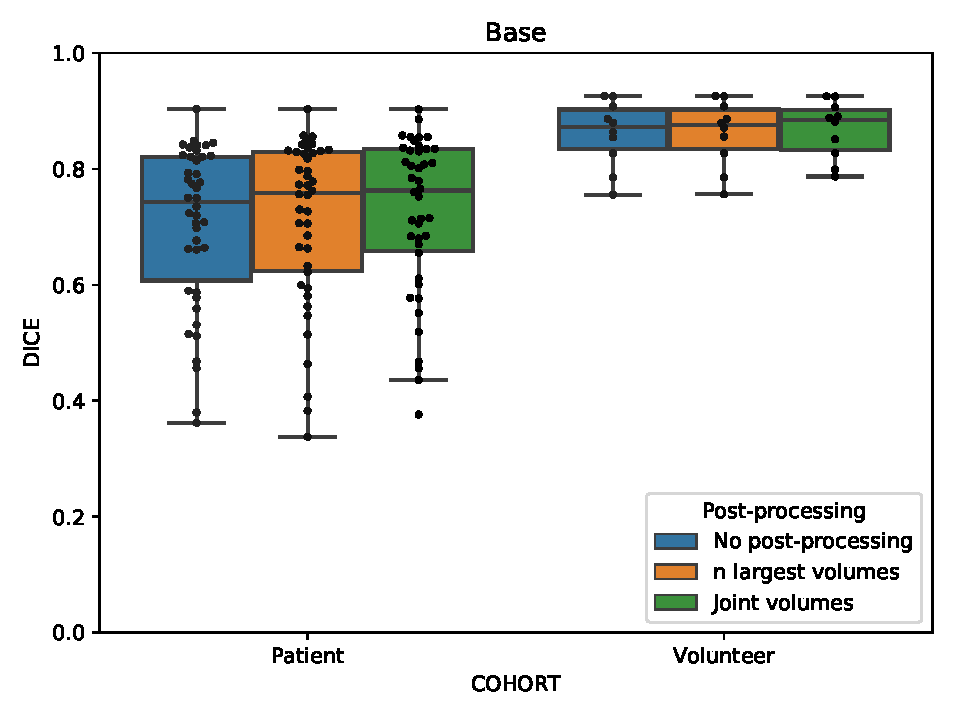
\includegraphics[width=0.7\textwidth]{pp_boxplot_base_DICE}
	}
	\hfill
	\subfloat[]
	{
		\label{fig:subfig:pp_boxplot_5to1_dice}
		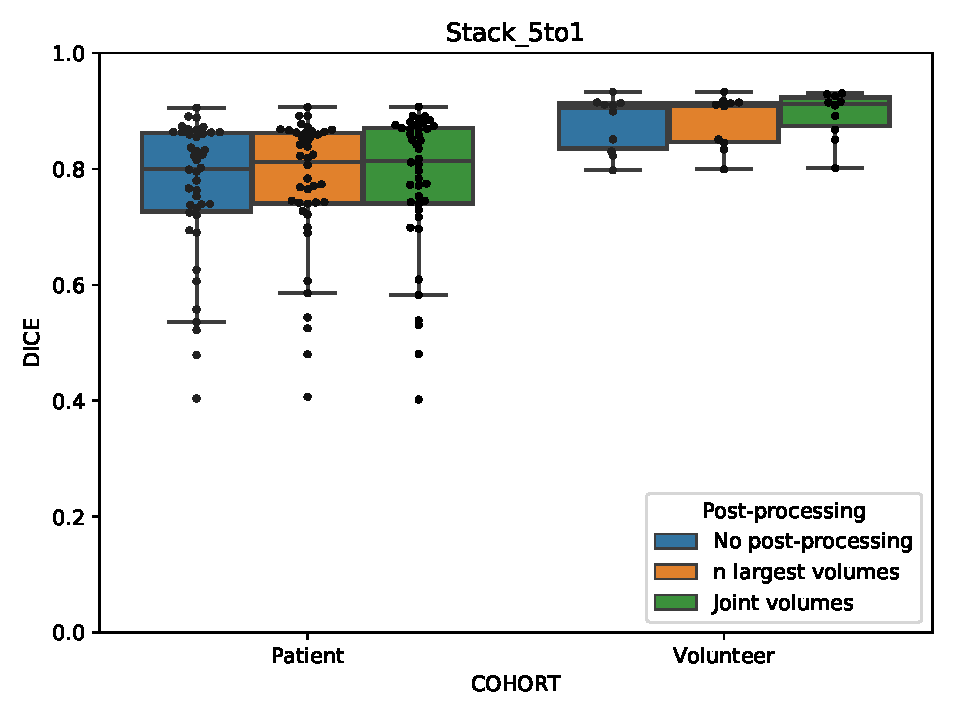
\includegraphics[width=0.7\textwidth]{pp_boxplot_5to1_DICE}
	}
	\caption[Post-processing impact on DICE]{}
	\label{fig:pp_boxplots_dice}  
\end{figure}

\begin{figure}[htbp]
	\centering
	\subfloat[]
	{
		\label{fig:subfig:pp_boxplot_base_vs}
		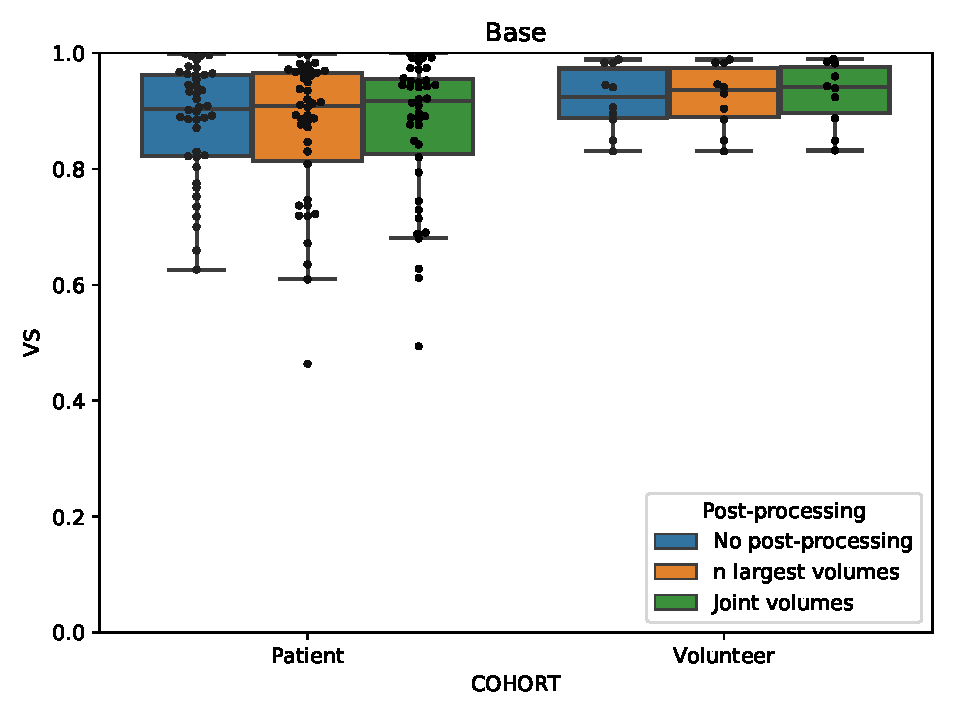
\includegraphics[width=0.7\textwidth]{pp_boxplot_base_VS}
	}
	\hfill
	\subfloat[]
	{
		\label{fig:subfig:pp_boxplot_5to1_vs}
		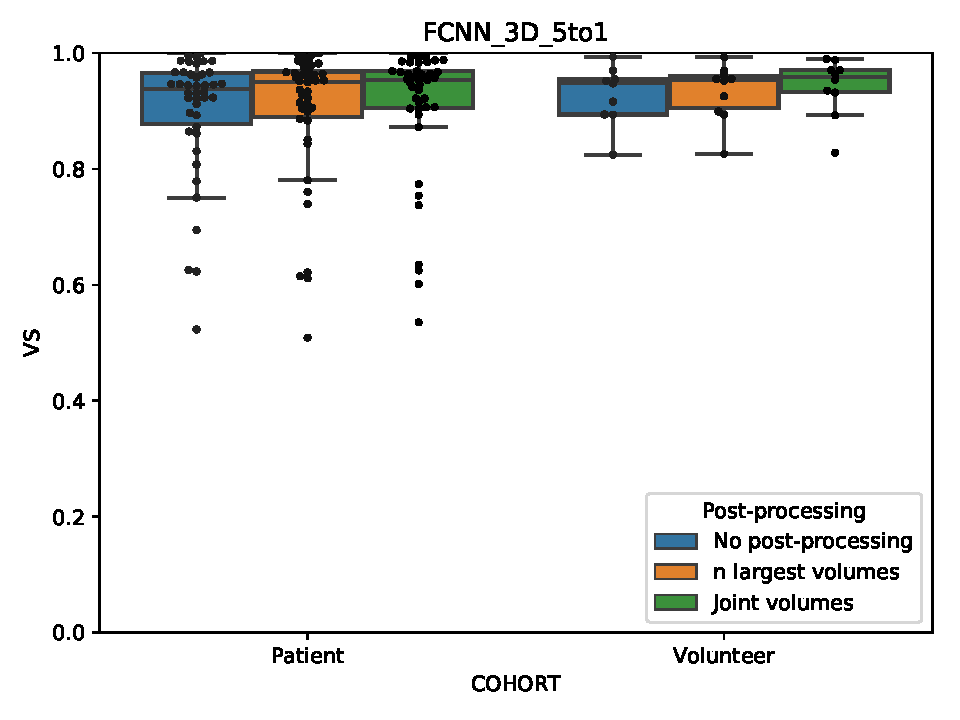
\includegraphics[width=0.7\textwidth]{pp_boxplot_5to1_VS}
	}
	\caption[Post-processing impact on VS]{}
	\label{fig:pp_boxplots_vs}  
\end{figure}

\begin{figure}[htbp]
	\centering
	\subfloat[]
	{
		\label{fig:subfig:pp_boxplot_base_avd}
		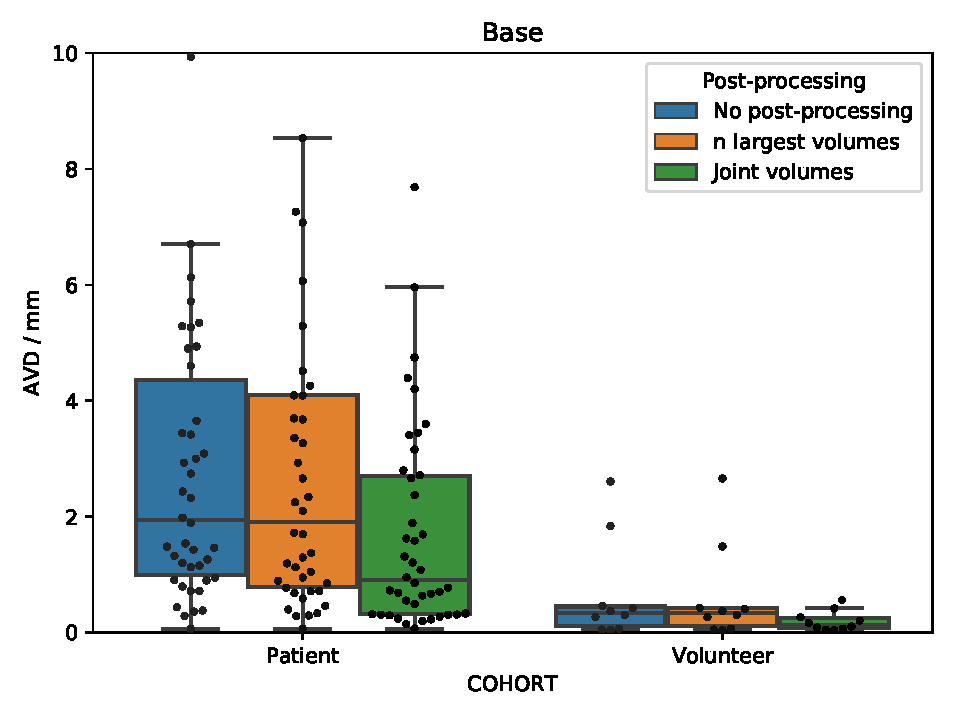
\includegraphics[width=0.7\textwidth]{pp_boxplot_base_AVD}
	}
	\hfill
	\subfloat[]
	{
		\label{fig:subfig:pp_boxplot_5to1_avd}
		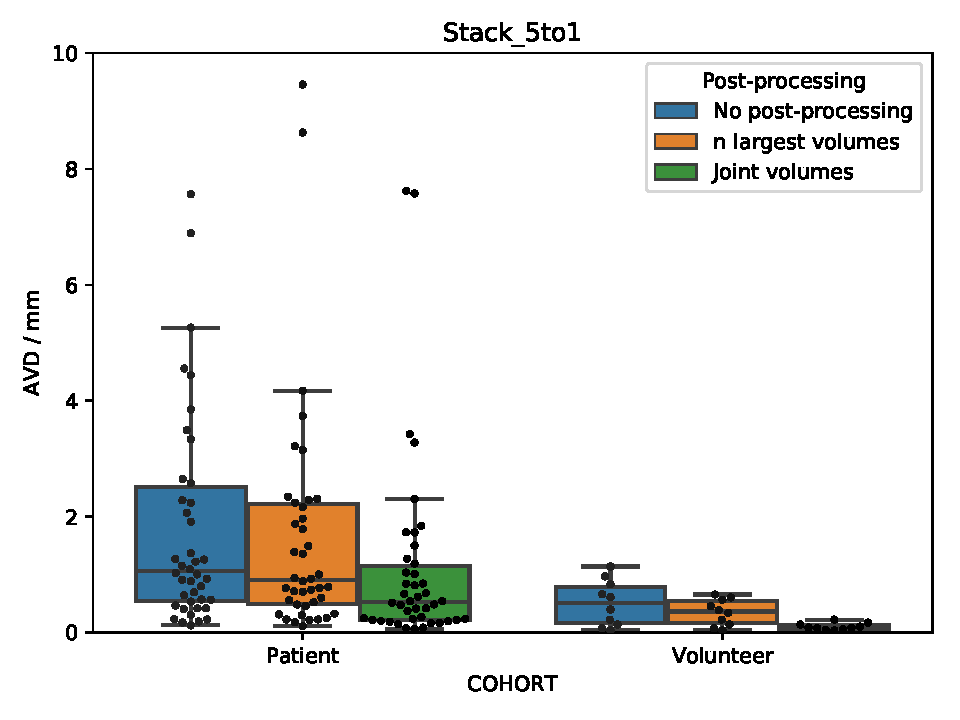
\includegraphics[width=0.7\textwidth]{pp_boxplot_5to1_AVD}
	}
	\caption[Post-processing impact on AVD]{}
	\label{fig:pp_boxplots_avd}  
\end{figure}

\begin{figure}[htbp]
	\centering
	\subfloat[]
	{
		\label{fig:subfig:pp_boxplot_base_hd95}
		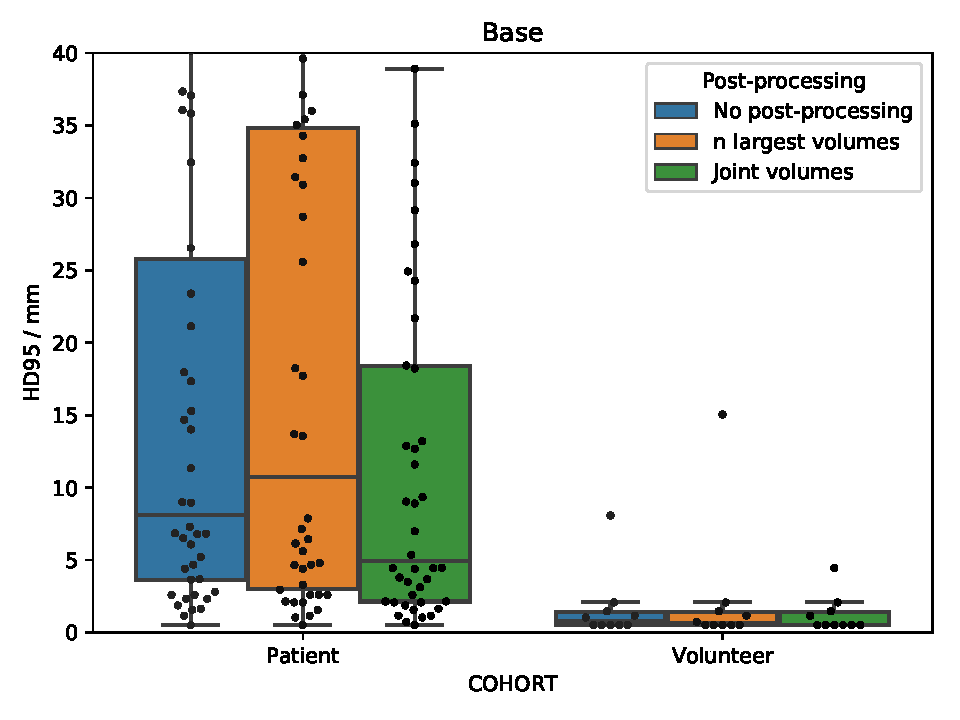
\includegraphics[width=0.7\textwidth]{pp_boxplot_base_HD95}
	}
	\hfill
	\subfloat[]
	{
		\label{fig:subfig:pp_boxplot_5to1_hd95}
		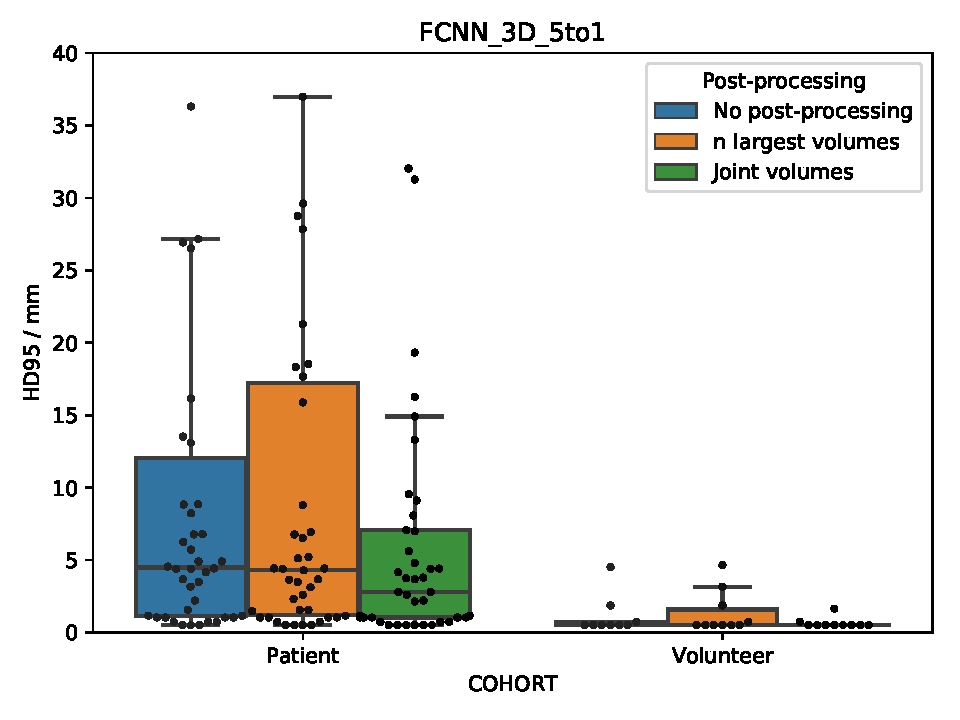
\includegraphics[width=0.7\textwidth]{pp_boxplot_5to1_HD95}
	}
	\caption[Post-processing impact on HD95]{}
	\label{fig:pp_boxplots_hd95}  
\end{figure}

\begin{figure}[htbp]
	\centering
	\subfloat[]
	{
		\label{fig:subfig:pp_boxplot_base_hd}
		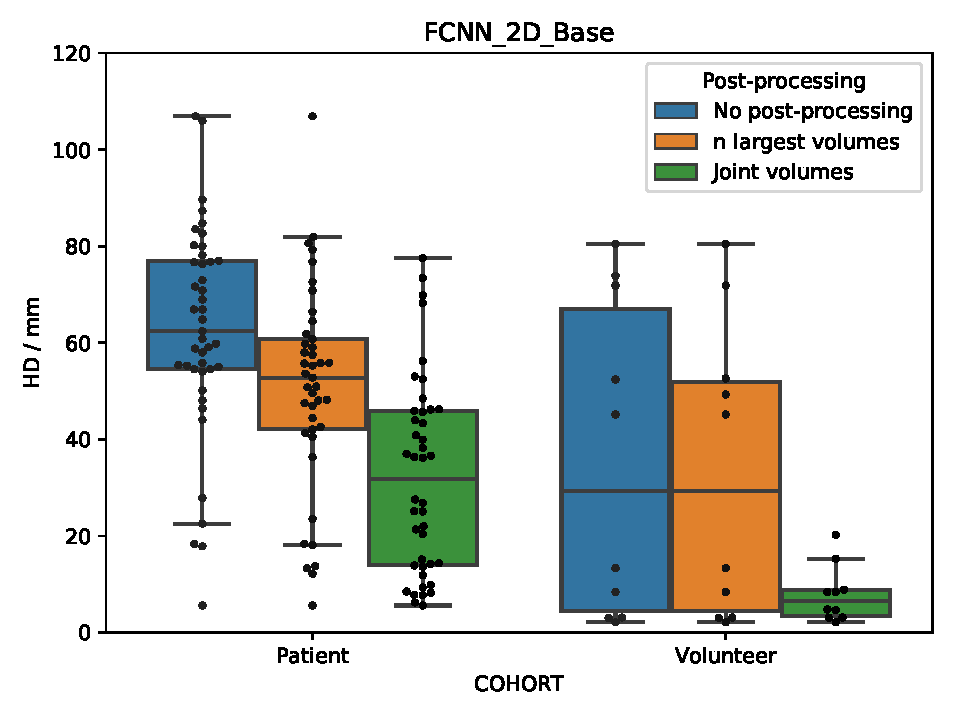
\includegraphics[width=0.7\textwidth]{pp_boxplot_base_HD}
	}
	\hfill
	\subfloat[]
	{
		\label{fig:subfig:pp_boxplot_5to1_hd}
		\includegraphics[width=0.7\textwidth]{pp_boxplot_5to1_HD}
	}
	\caption[Post-processing impact on HD]{}
	\label{fig:pp_boxplots_hd}  
\end{figure}

\section{Evaluation: FCNN and Raters} % =============================================================

\begin{figure}[htbp]	
	\includegraphics[width=\textwidth]{inter_rater}
    \caption[Inter-Rater Agreement]{Inter-rater agreement for the DICE, VS, AVD, HD95 and HD metrics. Values close to 1.00 for DICE and VS correspond to a high level of agreement between the raters. Conversely, low values for AVD, HD95 and HD imply higher level agreement.}
    \label{fig:inter_rater}
\end{figure}

\chapter{Network Architectures} % =================================================================================

\begin{sidewaystable}[htbp]
   \centering
   \caption[Architecture of FCNN 2D Baseline]{Detailed architecture of the baseline neural network.}
   \begin{tabular}{l*{4}{l}}
      \toprule
      Level	& Layer						& Properties 					& In 									& Out	\\
      		&							&								& $C \times D \times H \times W$		& $C \times D \times H \times W$		\\
      \midrule
      1D	& Conv2D, Dropout, BN, ReLU & K: $3 \times 3$, P1, S1		& $2 \times 1 \times 300 \times 300$	& $32 \times 1 \times 300 \times 300$	\\
      1D	& Conv2D, Dropout, BN, ReLU & K: $3 \times 3$, P1, S1		& $32 \times 1 \times 300 \times 300$	& $32 \times 1 \times 300 \times 300$	\\
      2D	& Max Pooling				& K: $2 \times 2$, P0, S2		& $32 \times 1 \times 300 \times 300$	& $32 \times 1 \times 150 \times 150$	\\
      2D	& Conv2D, Dropout, BN, ReLU & K: $3 \times 3$, P1, S1		& $32 \times 1 \times 150 \times 150$	& $64 \times 1 \times 150 \times 150$	\\
      2D	& Conv2D, Dropout, BN, ReLU & K: $3 \times 3$, P1, S1		& $64 \times 1 \times 150 \times 150$	& $64 \times 1 \times 150 \times 150$	\\
      3D	& Max Pooling				& K: $2 \times 2$, P0, S2		& $64 \times 1 \times 150 \times 150$	& $64 \times 1 \times 75 \times 75$		\\
      3D	& Conv2D, Dropout, BN, ReLU & K: $3 \times 3$, P1, S1		& $64 \times 1 \times 75 \times 75$		& $128 \times 1 \times 75 \times 75$	\\
      3D	& Conv2D, Dropout, BN, ReLU & K: $3 \times 3$, P1, S1		& $128 \times 1 \times 75 \times 75$	& $128 \times 1 \times 75 \times 75$	\\
      4D	& Max Pooling				& K: $2 \times 2$, P0, S2		& $128 \times 1 \times 75 \times 75$	& $128 \times 1 \times 37 \times 37$	\\
      4D	& Conv2D, Dropout, BN, ReLU & K: $3 \times 3$, P1, S1		& $128 \times 1 \times 37 \times 37$	& $256 \times 1 \times 37 \times 37$	\\
      4D	& Conv2D, Dropout, BN, ReLU & K: $3 \times 3$, P1, S1		& $256 \times 1 \times 37 \times 37$	& $256 \times 1 \times 37 \times 37$	\\
      5D	& Max Pooling				& K: $2 \times 2$, P0, S2		& $256 \times 1 \times 37 \times 37$	& $256 \times 1 \times 18 \times 18$	\\
      5D	& Conv2D, Dropout, BN, ReLU & K: $3 \times 3$, P1, S1		& $256 \times 1 \times 18 \times 18$	& $512 \times 1 \times 18 \times 18$	\\
      5D	& Conv2D, Dropout, BN, ReLU & K: $3 \times 3$, P1, S1		& $512 \times 1 \times 18 \times 18$	& $512 \times 1 \times 18 \times 18$	\\
      
      4U	& ConvTranspose2D			& K: $2 \times 2$, P0, S2		& $512 \times 1 \times 18 \times 18$	& $256 \times 1 \times 37 \times 37$	\\
      4U	& Concat Skip Feature Map	&								&										& $512 \times 1 \times 37 \times 37$	\\
      4U	& Conv2D, Dropout, BN, ReLU & K: $3 \times 3$, P1, S1		& $512 \times 1 \times 37 \times 37$	& $256 \times 1 \times 37 \times 37$	\\
      4U	& Conv2D, Dropout, BN, ReLU & K: $3 \times 3$, P1, S1		& $256 \times 1 \times 37 \times 37$	& $256 \times 1 \times 37 \times 37$	\\
      3U	& ConvTranspose2D			& K: $2 \times 2$, P0, S2		& $256 \times 1 \times 37 \times 37$	& $128 \times 1 \times 75 \times 75$	\\
      3U	& Concat Skip Feature Map	&								&										& $256 \times 1 \times 75 \times 75$	\\
      3U	& Conv2D, Dropout, BN, ReLU & K: $3 \times 3$, P1, S1		& $256 \times 1 \times 75 \times 75$	& $128 \times 1 \times 75 \times 75$	\\
      3U	& Conv2D, Dropout, BN, ReLU & K: $3 \times 3$, P1, S1		& $128 \times 1 \times 75 \times 75$	& $128 \times 1 \times 75 \times 75$	\\
      2U	& ConvTranspose2D			& K: $2 \times 2$, P0, S2		& $128 \times 1 \times 75 \times 75$	& $64 \times 1 \times 150 \times 150$	\\
      2U	& Concat Skip Feature Map	&								&										& $128 \times 1 \times 150 \times 150$	\\
      2U	& Conv2D, Dropout, BN, ReLU & K: $3 \times 3$, P1, S1		& $128 \times 1 \times 150 \times 150$	& $64 \times 1 \times 150 \times 150$	\\
      2U	& Conv2D, Dropout, BN, ReLU & K: $3 \times 3$, P1, S1		& $64 \times 1 \times 150 \times 150$	& $64 \times 1 \times 150 \times 150$	\\
      1U	& ConvTranspose2D			& K: $2 \times 2$, P0, S2		& $128 \times 1 \times 150 \times 150$	& $32 \times 1 \times 300 \times 300$	\\
      1U	& Concat Skip Feature Map	&								&										& $64 \times 1 \times 300 \times 300$	\\
      1U	& Conv2D, Dropout, BN, ReLU & K: $3 \times 3$, P1, S1		& $64 \times 1 \times 300 \times 300$	& $32 \times 1 \times 300 \times 300$	\\
      1U	& Conv2D, Dropout, BN, ReLU & K: $3 \times 3$, P1, S1		& $32 \times 1 \times 300 \times 300$	& $32 \times 1 \times 300 \times 300$	\\
      
      Out	& Conv2D					& K: $1 \times 1$, P0, S1		& $32 \times 1 \times 300 \times 300$	& $1 \times 1 \times 300 \times 300$	\\
      \bottomrule
   \end{tabular}
   \label{tab:architecture_fcnn_base}
\end{sidewaystable}

\begin{sidewaystable}[htbp]
   \centering
   \caption[Architecture of FCNN 3D Volumetric]{Detailed architecture of the volumetric neural network. $I$, $O$ correspond to the chosen number of input and output slices, respectively. The following combinations have been trained: $I = 3$, $O = 1$ (3-to-1), $I = 5$, $O = 1$ (5-to-1), $I = 5$, $O = 3$ (5-to-3).}
   \begin{tabular}{l*{4}{l}}
      \toprule
      Level	& Layer				& Properties 					& In							& Out									\\
      &							&								& $C \times D \times H \times W$& $C \times D \times H \times W$		\\
      \midrule
      1D	& Conv3D, Dropout, BN, ReLU & K: $1 \times 3 \times 3$, P(0, 1, 1), S1	& $2 \times I \times 300 \times 300$	& $32 \times I \times 300 \times 300$	\\
      1D	& Conv3D, Dropout, BN, ReLU & K: $3 \times 3 \times 3$, P1, S1			& $32 \times I \times 300 \times 300$	& $32 \times I \times 300 \times 300$	\\
      2D	& Max Pooling				& K: $1 \times 2 \times 2$, P0, S(1, 2, 2)	& $32 \times I \times 300 \times 300$	& $32 \times I \times 150 \times 150$	\\
      2D	& Conv3D, Dropout, BN, ReLU & K: $1 \times 3 \times 3$, P(0, 1, 1), S1	& $32 \times I \times 150 \times 150$	& $64 \times I \times 150 \times 150$	\\
      2D	& Conv3D, Dropout, BN, ReLU & K: $3 \times 3 \times 3$, P1, S1			& $64 \times I \times 150 \times 150$	& $64 \times I \times 150 \times 150$	\\
      3D	& Max Pooling				& K: $1 \times 2 \times 2$, P0, S(1, 2, 2)	& $64 \times I \times 150 \times 150$	& $64 \times I \times 75 \times 75$		\\
      3D	& Conv3D, Dropout, BN, ReLU & K: $1 \times 3 \times 3$, P(0, 1, 1), S1	& $64 \times I \times 75 \times 75$		& $128 \times I \times 75 \times 75$	\\
      3D	& Conv3D, Dropout, BN, ReLU & K: $3 \times 3 \times 3$, P1, S1			& $128 \times I \times 75 \times 75$	& $128 \times I \times 75 \times 75$	\\
      4D	& Max Pooling				& K: $1 \times 2 \times 2$, P0, S(1, 2, 2)	& $128 \times I \times 75 \times 75$	& $128 \times I \times 37 \times 37$	\\
      4D	& Conv3D, Dropout, BN, ReLU & K: $1 \times 3 \times 3$, P(0, 1, 1), S1	& $128 \times I \times 37 \times 37$	& $256 \times I \times 37 \times 37$	\\
      4D	& Conv3D, Dropout, BN, ReLU & K: $3 \times 3 \times 3$, P1, S1			& $256 \times I \times 37 \times 37$	& $256 \times I \times 37 \times 37$	\\
      5D	& Max Pooling				& K: $1 \times 2 \times 2$, P0, S(1, 2, 2)	& $256 \times I \times 37 \times 37$	& $256 \times I \times 18 \times 18$	\\
      5D	& Conv3D, Dropout, BN, ReLU & K: $1 \times 3 \times 3$, P(0, 1, 1), S1	& $256 \times I \times 18 \times 18$	& $512 \times I \times 18 \times 18$	\\
      5D	& Conv3D, Dropout, BN, ReLU & K: $3 \times 3 \times 3$, P1, S1			& $512 \times I \times 18 \times 18$	& $512 \times I \times 18 \times 18$	\\
      
      4U	& ConvTranspose3D			& K: $1 \times 2 \times 2$, P0, S(1, 2, 2)	& $512 \times I \times 18 \times 18$	& $256 \times I \times 37 \times 37$	\\
      4U	& Concat Skip Feature Map	&											&										& $512 \times I \times 37 \times 37$	\\
      4U	& Conv3D, Dropout, BN, ReLU & K: $1 \times 3 \times 3$, P(0, 1, 1), S1	& $512 \times I \times 37 \times 37$	& $256 \times I \times 37 \times 37$	\\
      4U	& Conv3D, Dropout, BN, ReLU & K: $3 \times 3 \times 3$, P1, S1			& $256 \times I \times 37 \times 37$	& $256 \times I \times 37 \times 37$	\\
      3U	& ConvTranspose3D			& K: $1 \times 2 \times 2$, P0, S(1, 2, 2)	& $256 \times I \times 37 \times 37$	& $128 \times I \times 75 \times 75$	\\
      3U	& Concat Skip Feature Map	&											&										& $256 \times I \times 75 \times 75$	\\
      3U	& Conv3D, Dropout, BN, ReLU & K: $1 \times 3 \times 3$, P(0, 1, 1), S1	& $256 \times I \times 75 \times 75$	& $128 \times I \times 75 \times 75$	\\
      3U	& Conv3D, Dropout, BN, ReLU & K: $3 \times 3 \times 3$, P1, S1			& $128 \times I \times 75 \times 75$	& $128 \times I \times 75 \times 75$	\\
      2U	& ConvTranspose3D			& K: $1 \times 2 \times 2$, P0, S(1, 2, 2)	& $128 \times I \times 75 \times 75$	& $64 \times I \times 150 \times 150$	\\
      2U	& Concat Skip Feature Map	&											&										& $128 \times I \times 150 \times 150$	\\
      2U	& Conv3D, Dropout, BN, ReLU & K: $1 \times 3 \times 3$, P(0, 1, 1), S1	& $128 \times I \times 150 \times 150$	& $64 \times I \times 150 \times 150$	\\
      2U	& Conv3D, Dropout, BN, ReLU & K: $3 \times 3 \times 3$, P1, S1			& $64 \times I \times 150 \times 150$	& $64 \times I \times 150 \times 150$	\\
      1U	& ConvTranspose2D			& K: $1 \times 2 \times 2$, P0, S(1, 2, 2)	& $128 \times I \times 150 \times 150$	& $32 \times I \times 300 \times 300$	\\
      1U	& Concat Skip Feature Map	&											&										& $64 \times I \times 300 \times 300$	\\
      1U	& Conv3D, Dropout, BN, ReLU & K: $1 \times 3 \times 3$, P(0, 1, 1), S1	& $64 \times I \times 300 \times 300$	& $32 \times I \times 300 \times 300$	\\
      1U	& Conv3D, Dropout, BN, ReLU & K: $3 \times 3 \times 3$, P1, S1			& $32 \times I \times 300 \times 300$	& $32 \times I \times 300 \times 300$	\\
      			
      Out	& Conv3D					& K: $I \times 1 \times 1$, P0, S1			& $32 \times I \times 300 \times 300$	& $1 \times O \times 300 \times 300$	\\
      \bottomrule
   \end{tabular}
   \label{tab:architecture_fcnn_volumetric}
\end{sidewaystable}

\begin{sidewaystable}[htbp]
   \centering
   \caption[Architecture of FCNN 3D Patches]{Detailed architecture of the patch-based neural network.}
   \begin{tabular}{l*{4}{l}}
      \toprule
      Level	& Layer						& Properties 					& In							& Out									\\
      		&							&								& $C \times D \times H \times W$& $C \times D \times H \times W$		\\
      \midrule
      1D	& Conv2D, Dropout, BN, ReLU & K: $3 \times 3 \times 3$, P1, S1			& $2 \times 12 \times 128 \times 128$	&	$32 \times 12 \times 128 \times 128$	\\
      1D	& Conv2D, Dropout, BN, ReLU & K: $3 \times 3 \times 3$, P1, S1			& $32 \times 12 \times 128 \times 128$	&	$32 \times 12 \times 128 \times 128$	\\
      2D	& Max Pooling				& K: $1 \times 2 \times 2$, P0, S(1, 2, 2)	& $32 \times 12 \times 128 \times 128$	&	$32 \times 12 \times 64 \times 64$	\\
      2D	& Conv2D, Dropout, BN, ReLU & K: $3 \times 3 \times 3$, P1, S1			& $32 \times 12 \times 64 \times 64$	&	$64 \times 12 \times 64 \times 64$	\\
      2D	& Conv2D, Dropout, BN, ReLU & K: $3 \times 3 \times 3$, P1, S1			& $64 \times 12 \times 64 \times 64$	& 	$64 \times 12 \times 64 \times 64$	\\
      3D	& Max Pooling				& K: $1 \times 2 \times 2$, P0, S(1, 2, 2)	& $64 \times 12 \times 64 \times 64$	& 	$64 \times 12 \times 32 \times 32$		\\
      3D	& Conv2D, Dropout, BN, ReLU & K: $3 \times 3 \times 3$, P1, S1			& $64 \times 12 \times 32 \times 32$	&	$128 \times 12 \times 32 \times 32$	\\
      3D	& Conv2D, Dropout, BN, ReLU & K: $3 \times 3 \times 3$, P1, S1			& $128 \times 12 \times 32 \times 32$	&	$128 \times 12 \times 32 \times 32$	\\
      4D	& Max Pooling				& K: $1 \times 2 \times 2$, P0, S(1, 2, 2)	& $128 \times 12 \times 32 \times 32$	&	$128 \times 12 \times 16 \times 16$	\\
      4D	& Conv2D, Dropout, BN, ReLU & K: $3 \times 3 \times 3$, P1, S1			& $128 \times 12 \times 16 \times 16$	&	$256 \times 12 \times 16 \times 16$	\\
      4D	& Conv2D, Dropout, BN, ReLU & K: $3 \times 3 \times 3$, P1, S1			& $256 \times 12 \times 16 \times 16$	&	$256 \times 12 \times 16 \times 16$	\\
      
      3U	& ConvTranspose2D			& K: $1 \times 2 \times 2$, P0, S(1, 2, 2)	& $256 \times 12 \times 16 \times 16$	& $128 \times 12 \times 32 \times 32$	\\
      3U	& Concat Skip Feature Map	&								&													& $256 \times 12 \times 32 \times 32$	\\
      3U	& Conv2D, Dropout, BN, ReLU & K: $3 \times 3 \times 3 \times 3$, P1, S1	& $256 \times 12 \times 32 \times 32$	& $128 \times 12 \times 32 \times 32$	\\
      3U	& Conv2D, Dropout, BN, ReLU & K: $3 \times 3 \times 3 \times 3$, P1, S1	& $128 \times 12 \times 32 \times 32$	& $128 \times 12 \times 32 \times 32$	\\
      2U	& ConvTranspose2D			& K: $1 \times 2 \times 2$, P0, S(1, 2, 2)	& $128 \times 12 \times 32 \times 32$	& $64 \times 12 \times 64 \times 64$	\\
      2U	& Concat Skip Feature Map	&								&													& $128 \times 12 \times 64 \times 64$	\\
      2U	& Conv2D, Dropout, BN, ReLU & K: $3 \times 3 \times 3 \times 3$, P1, S1	& $128 \times 12 \times 64 \times 64$	& $64 \times 12 \times 64 \times 64$	\\
      2U	& Conv2D, Dropout, BN, ReLU & K: $3 \times 3 \times 3 \times 3$, P1, S1	& $64 \times 12 \times 64 \times 64$	& $64 \times 12 \times 64 \times 64$	\\
      1U	& ConvTranspose2D			& K: $1 \times 2 \times 2$, P0, S(1, 2, 2)	& $128 \times 12 \times 64 \times 64$	& $32 \times 12 \times 128 \times 128$	\\
      1U	& Concat Skip Feature Map	&								&													& $64 \times 12 \times 128 \times 128$	\\
      1U	& Conv2D, Dropout, BN, ReLU & K: $3 \times 3 \times 3 \times 3$, P1, S1	& $64 \times 12 \times 128 \times 128$	& $32 \times 12 \times 128 \times 128$	\\
      1U	& Conv2D, Dropout, BN, ReLU & K: $3 \times 3 \times 3 \times 3$, P1, S1	& $32 \times 12 \times 128 \times 128$	& $32 \times 12 \times 128 \times 128$	\\
      
      Out	& Conv2D					& K: $1 \times 1 \times 1$, P0, S1			& $32 \times 12 \times 128 \times 128$	& $1 \times 12 \times 128 \times 128$	\\
      \bottomrule
   \end{tabular}
   \label{tab:architecture_fcnn_patches}
\end{sidewaystable}

\chapter{Additional Tables} % =====================================================================================

\begin{table}[htbp]
   \centering
   \caption{Assignment of subjects to the different folds for the four-fold cross-validation.}
   \begin{tabular}{p{3cm}l}
      \toprule
      \textbf{Fold-0} & $n = 13$ \\      
      Subject & Cohort \\
      \midrule
      05B           & Volunteer \\
      25A           & Volunteer \\
      012\_V0\_R1  & Patient   \\
      037\_V0\_R2  & Patient   \\
      044\_V0\_R4  & Patient   \\
      084\_V0\_R3  & Patient   \\
      159\_V0\_R3 & Patient   \\
      173\_V0\_R4 & Patient   \\
      174\_V0\_R4 & Patient   \\
      199\_V0\_R2 & Patient   \\
      221\_V0\_R3 & Patient   \\
      229\_V0\_R3 & Patient   \\
      231\_V0\_R4 & Patient   \\
      \bottomrule
   \end{tabular}
   \begin{tabular}{p{3cm}l}      
      \toprule
      \textbf{Fold-1} & $n = 13$ \\
      Subject & Cohort \\
      \midrule
      05A           & Volunteer \\
      12A           & Volunteer \\
      013\_V0\_R3  & Patient   \\
      022\_V0\_R3  & Patient   \\
      034\_V1\_R3  & Patient   \\
      161\_V0\_R3 & Patient   \\
      166\_V0\_R4 & Patient   \\
      167\_V0\_R3 & Patient   \\
      192\_V0\_R2 & Patient   \\
      213\_V0\_R4 & Patient   \\
      218\_V0\_R3 & Patient   \\
      220\_V0\_R1 & Patient   \\
      222\_V0\_R1 & Patient   \\      
      \bottomrule
   \end{tabular}
   \begin{tabular}{p{3cm}l}
      \textbf{Fold-2} & $n = 13$ \\
      Subject & Cohort \\
      \midrule
      12B           & Volunteer \\
      13A           & Volunteer \\
      24A           & Volunteer \\
      049\_V0\_R3  & Patient   \\
      062\_V0\_R3  & Patient   \\
      153\_V0\_R3 & Patient   \\
      158\_V0\_R3 & Patient   \\
      160\_V0\_R1 & Patient   \\
      166\_V0\_R5 & Patient   \\
      171\_V0\_R1 & Patient   \\
      201\_V0\_R1 & Patient   \\
      219\_V0\_R4 & Patient   \\
      222\_V1\_R2 & Patient   \\      
      \bottomrule
   \end{tabular}
   \begin{tabular}{p{3cm}l}
      \textbf{Fold-3} & $n = 13$ \\
      Subject & Cohort \\
      \midrule
      13B           & Volunteer \\
      24B           & Volunteer \\
      25B           & Volunteer \\
      013\_V0\_R2  & Patient   \\
      019\_V0\_R3  & Patient   \\
      036\_V1\_R1  & Patient   \\
      062\_V1\_R3  & Patient   \\
      172\_V0\_R4 & Patient   \\
      180\_V0\_R3 & Patient   \\
      195\_V0\_R1 & Patient   \\      
      215\_V0\_R1 & Patient   \\
      219\_V0\_R3 & Patient   \\
      230\_V0\_R3 & Patient   \\      
      \bottomrule
   \end{tabular}
   \label{tab:fold_assignment}
\end{table}

\begin{sidewaystable}[htbp]
   \centering
   \caption[Hyperparameters]{The used hyperparemeters for the different network architectures we trained.}
   \begin{tabular}{l*{7}{l}}
      \toprule
      Neural Network & Epochs	& Batchsize & Learning Rate & Steps & Momentum & In & Out \\
      		&			&	&	&	&	& $D \times H \times W$	&  $D \times H \times W$	\\
      \midrule
      FCNN\_2D\_Base	& 150	& 32	& 0.001	& 100, 125 & 0.99	& $1 \times 300 \times 300$	& $1 \times 300 \times 300$ \\
      \midrule
      FCNN\_3D\_3to1 & 200	& 8	& 0.0001 & 180, 190 & 0.99 & $3 \times 300 \times 300$ & $1 \times 300 \times 300$ \\
      FCNN\_3D\_5to1 	& 200	& 8	& 0.0001 & 180, 190 & 0.99 & $5 \times 300 \times 300$ & $1 \times 300 \times 300$ \\
      FCNN\_3D\_5to3 	& 200	& 6	& 0.0001 & 180, 190 & 0.99 & $5 \times 300 \times 300$ & $3 \times 300 \times 300$ \\
      FCNN\_3D\_Patch & 500	& 16	& 0.0001 & 400, 450 & 0.99 & $12 \times 128 \times 128$ & $12 \times 128 \times 128$ \\
      FCNN\_3D\_Proj & 200	& 6	& 0.0001 & 180, 190 & 0.99 & $5 \times 300 \times 300$ & $3 \times 300 \times 300$ \\
      \bottomrule
   \end{tabular}
   \label{tab:hyperparameters}
\end{sidewaystable}





\end{appendix}

\end{document}

\endinput